\documentclass{MScthesisITEM}

% this package is just to generate text for demo-purposes
\usepackage{blindtext}
\usepackage{ae}
%\usepackage[footnote,draft,silent,nomargin]{fixme}
\usepackage[draft,silent,nomargin]{fixme} %No output
\usepackage{csquotes} %to quote in a good way
\usepackage{eurosym}
\usepackage{booktabs} %nice tabulars
\usepackage{multirow} %nice tabulars
\usepackage{siunitx} %nice si units
\usepackage{listing} %nice code

%% New context definiton
\newcommand{\code}{\texttt} %Inline code snippet
\newcommand{\name}{}   %Person name
\newcommand{\comp}{\emph}   %Company name
\newcommand{\proj}{}   %Project name
\newcommand{\prog}{\texttt}   %Program name

%% Better tables
\renewcommand{\arraystretch}{1.2}

\title{GSM and GPRS Security Using OsmocomBB} % The title of your assignement; NB use \newlinetitle to start a newline
\author{François Pönsgen} % Your firstname and lastname
\professor{Stig F. Mjølsnes, ITEM (NTNU)} % Affiliation = ITEM for instance
\supervisor{Jean-Michel Dricot, OPERA (ULB)}

%% Uncomment the following in case you want subfigures; note that there will be a warning for the caption package
% \let\subcaption\undefined
% \let\subfloat\undefined
% \usepackage[bf]{caption}
% \usepackage{subcaption}

\DeclareGraphicsExtensions{.pdf,.jpg,.png}
\graphicspath{{../img/}}

\loadglsentries{glossary}
\makeglossaries

\begin{document}
\selectlanguage{english}
\pagenumbering{roman}
\pagestyle{plain}

%% Only for the project; comment out the line below for the master's thesis; the front page will be generated automatically by DAIM
%\titleITEM

%% Only for the master's thesis; for the project report the description is taken from It's Learning and added by the department
\selectlanguage{english} % Change to 'norsk' if you are writing in Norwegian
\begin{titlingpage}

\noindent
\begin{tabular}{@{}p{4cm}l}
\textbf{Title:} 	& \thetitle \\
\textbf{Student:}	& \theauthor \\
\end{tabular}

\vspace{4ex}
\noindent\textbf{Problem description:}
\vspace{2ex}

\noindent 

The OsmocomBB project~\cite{osmocombb_2015} aims to create a free
and open source GSM baseband software implementation, which enhances
cheap and accessible compatible phones by giving access to their inner
workings. Thus, it can be used to analyze GSM and GPRS security
functionalities.

There are four goals to this thesis and the first one is to set up and
understand the OsmocomBB software, and to use it to acquire a solid
practical knowledge of GSM and GPRS with a focus on the security
aspects. The second one is to reproduce and understand the feasibility
and efficiency of a passive attack~\cite{munaut_wideband_2010} which
uses a modified version of OsmocomBB along with cheap compatible mobile
phones to eavesdrop on GSM. The third goal is to do the same with
another passive attack~\cite{melette_gprs_2011} which allows to
eavesdrop on GPRS using almost the same set of tools. Finally, the last
goal is to analyze the security configuration of mobile networks at
various locations and to check whether mobile operators implemented
solutions to prevent these attacks.

\vspace{6ex}

\noindent
\begin{tabular}{@{}p{4cm}l}
\textbf{Responsible professor:} 	& \theprofessor \\
\textbf{Supervisor at ULB:}			& \thesupervisor \\
\end{tabular}

\end{titlingpage}

\cleardoublepage

%% There must be an abstract in English, even though the main text is in Norwegian
\selectlanguage{english}
\pagestyle{empty}
\begin{abstract}


This thesis analyzes the security of Norwegian GSM and GPRS networks
using the OsmocomBB project and considering two types of attacks: an
eavesdropping attack, and a set of Denial-of-Service attacks. OsmocomBB
aims to create a free and open source GSM baseband software
implementation. Doing so, it enhances cheap and accessible compatible
phones by giving access to their inner workings. The eavesdropping
attack was presented at the 27th Chaos Communication Congress by Silvain
Munaut and Karsten Nohl. The set of Denial-of-Service attacks is
composed of: the RACH flood attack, the IMSI attach flood attack, the
IMSI detach attack, and an attack based on race conditions in the paging
process.

This thesis first introduces the projects which are related to
\proj{OsmocomBB}, and offers a guide into the GSM system by linking the
specifications with the \proj{OsmocomBB} source code. Then, it describes
the eavesdropping and Denial-of-Service attacks in details. Some steps
of the eavesdropping attack as well as the first three Denial-of-Service
attacks are implemented. Finally, the results of measurements and
experiments conducted on Norwegian networks to assess the feasibility of
the attacks are presented.

It was found that both \comp{Telenor} and \comp{Netcom} seem protected
from the eavesdropping attack, since they renegotiate a TMSI for each
service and provide the A5/3 encryption algorithm. The IMSI detach
attack was the only Denial-of-Service attack tested on these networks,
since it targets a single user. It is effective on the Telenor network,
but not on the Netcom network. The other Denial-of-Service attacks are
probably effective, but were not tested since they could damage the
networks.

\end{abstract}

\cleardoublepage

%% Only for the master's thesis; if the main text is in English and you can write Norwegian, there must be an abstract in Norwegian as well.
% \selectlanguage{norsk}
% \include{abstract_norwegian}
% \cleardoublepage

\selectlanguage{english}% Change to 'norsk' if you are writing in Norwegian

\renewcommand{\abstractname}{Preface}
\begin{abstract}

  This Master's thesis is the result of researches carried out over 22
  weeks during the spring semester in the Department of Telematics at
  the Norwegian University of Science and Technology. The NTNU has been
  my host university during a yearlong Erasmus exchange program, but
  this thesis is a requirement for the acquisition of the MSc in
  Electronics and Information Technology Engineering degree in the joint
  program between the two universities of Brussels: the Université
  Libre de Bruxelles, and the Vrije Universiteit Brussel.

  I would like to thank the people who helped me during these few
  months. Stig F. Mjølsnes, who gave me relevant advices, and guided me
  in the difficult process of academic writing. Jean-Michel Dricot, for
  introducing me to cellular networks and making this topic as
  interesting as he did. Many thanks also to all the \proj{OsmocomBB}
  developers for working on that great project, and to all the people
  who provided feedback during the writing process, especially Charles,
  Héloïse, and Pete. Finally, thanks a lot to Carole for supporting me!

  This thesis is distributed in the hope that it will be useful.

\end{abstract}

\cleardoublepage

% similarly you may add a separate acknowledgments page

\tableofcontents*
\cleardoublepage

%% include if relevant
%\listoffigures
%\cleardoublepage

%% include if relevant
%\listoftables
%\cleardoublepage

%% include if relevant
%\listofalgorithms
%\addcontentsline{toc}{chapter}{List of Algorithms}
%\cleardoublepage

%% include if relevant
%\printglossary[title=List of Symbols, style=long]
%\cleardoublepage
%\glsaddall[]

%%\clearpage
%\listoffixmes

%% include if relevant
\printglossary[title=List of Acronyms,type=\acronymtype] % prints just the list of acronyms
\cleardoublepage

\pagenumbering{arabic}
\pagestyle{ruled}
\chapter{Introduction} \label{chap:introduction}

%starting points, objective, results, conclusion
  
%http://www.theregister.co.uk/2012/11/09/20_years_of_gsm_digital_phones/
  %http://www.euronews.com/2015/06/01/belgium-hanging-up-on-the-phone-booth/
  %http://www.fiercewireless.com/europe/story/frances-operators-sign-accord-cover-all-mobile-not-spots-2020/2015-05-22?utm_medium=rss&utm_source=rss&utm_campaign=rss
  %http://www.fiercewireless.com/story/facebook-launches-facebook-lite-app-designed-2g-networks-emerging-markets/2015-01-27
  %http://indianexpress.com/article/technology/social/exclusive-skype-to-roll-out-made-for-india-app/
  %http://www.fiercewireless.com/europe/story/telenor-norway-will-ditch-3g-2g-lte-rollouts-gather-pace-northern-territori/2015-06-03?utm_medium=rss&utm_source=rss&utm_campaign=rss

  More than 20 years after its introduction, the \gls{gsm} is still
  relevant as a cheap and effective legacy system~\cite{cox_20_2012}.
  While phone booths are gradually removed from the streets, \gls{gsm}
  is now considered by some countries as a backup communication system
  which should be available everywhere, and might outlive
  3G~\cite{belgium:_2015,morris_frances_2015,carroll_telenor_2015}.
  Moreover, \gls{gprs} is still widely used in developing countries:
  \comp{Skype} or \comp{Facebook} recently provided specifically
  designed versions of their mobile applications aimed at the 2G data
  rate~\cite{goldstein_facebook_2015,swami_exclusive:_2015}.

  Yet, 20 years is a really long time in technology, and it shows. When
  \gls{gsm} networks were first deployed, the equipment was so expensive
  that it could only be acquired by phone operators. Now that cheap
  equipment and \gls{foss} projects are available, a wide attack surface
  is accessible. One of this project is \proj{OsmocomBB}, which provides
  a \gls{foss} implementation of a \gls{gsm} protocol stack. The
  motivation behind this thesis is to explore the impact of this project
  on the security of \gls{gsm} and \gls{gprs}. 

  \section{Problem description evolution}
  \label{sec:pb}

  The problem description defined originally and included at the
  beginning of this thesis had to be adapted along the way. This was
  done to follow the evolution of the work and the better understanding
  of the systems and their capabilities. The objective of this thesis
  was: exploring the available eavesdropping attacks on \gls{gsm} and
  \gls{gprs} using \proj{OsmocomBB}. This objective was modified in two
  ways. Firstly, the focus was switched to mostly consider \gls{gsm} at
  the expense of \gls{gprs}. Secondly, a new set of attacks was
  considered.

  The focus of this thesis on the security of \gls{gprs} was reduced for
  several reasons. Firstly, \gls{gprs} is not supported by
  \proj{OsmocomBB} yet, which makes attacks on this network very hard to
  implement. Secondly, the eavesdropping attack on \gls{gprs} has
  several major limitations, and is thus less interesting than first
  expected. Finally, the \gls{gprs} network is almost completely
  separated from the \gls{gsm} network, and a lot of work would have
  been needed to cover it too. Therefore, the emphasis is clearly on
  \gls{gsm}, but the impact on \gls{gprs} is considered as well. The
  focus also shifted from the eavesdropping attacks to a wider range of
  attacks that could be implemented with \proj{OsmocomBB}. A complete
  chapter is dedicated to \gls{dos} attacks, which appeared to be very
  relevant to the topic.

  The four goals originally defined are mostly accomplished. A solid
  practical knowledge had to be developed in order to implement the
  various attacks demonstrated in this thesis. The eavesdropping attack
  on \gls{gsm} was described in details and some steps were implemented,
  but it could not be executed completely. The only public demonstration
  of this attack was performed by \name{Sylvain Munaut}, and no
  implementation or detailed description were publicly available, which
  made this task harder. The eavesdropping attack on \gls{gprs} is a
  variation of the previous one and is therefore described as well, but
  was not tested. Finally, the feasibility of the attacks on Norwegian
  networks was investigated in details, and extended to \gls{dos}
  attacks. The organization of this thesis is described in the next
  section.

  \section{Structure}

  %Report this in chapter introductions.
    This thesis contains eight chapters. \Cref{chap:introduction}, the
    chapter you are reading, introduces the problem, the structure, and
    the methodology of the thesis. \Cref{chap:related_projects} gives
    references to the relevant researches in the field, and provides
    some context around \proj{OsmocomBB} by presenting important related
    projects.

    \Cref{chap:network_architecture} is meant to outline the \gls{gsm}
    and \gls{gprs} networks architectures, and to provide background for
    the following chapters. \Cref{chap:protocol_stack_implementation}
    gives an overview of the protocol stack running on the mobile
    phones, and provides links between the \proj{OsmocomBB} source code
    and the \gls{3gpp} specifications.

    After two theoretical chapters, \Cref{chap:eavesdropping_attacks} is
    mostly dedicated to an eavesdropping attack on \gls{gsm}, but also
    discusses an attack on \gls{gprs}. It details the various steps of
    the attacks and provides an implementation using \proj{OsmocomBB}
    for some of them. \Cref{chap:dos_attacks} is dedicated to \gls{dos}
    attacks using \proj{OsmocomBB}. It provides a description of the
    attacks as well as an implementation for most of them. They are
    aimed at the \gls{gsm} network, but can indirectly impact the
    \gls{gprs} network as well.

    \Cref{chap:security_configuration_of_norwegian_operators} assesses
    the feasibility of these two categories of attacks on Norwegian
    networks. It offers a detailed investigation using the
    implementations introduced in the previous chapters. Finally,
    \Cref{chap:conclusion} is the conclusion. It summarizes the thesis,
    gets back to its limitations and suggests possible future work.
    Appendices are available at the very end of this document, and
    contain a tutorial on the installation and usage of
    \proj{OsmocomBB}, the patches adding the proposed implementations,
    and a small case study on IMSI-catchers detection.

  \section{Methodology}

    The researches presented in this thesis are based on software.
    Therefore, the applied methodology is based on classical software
    engineering procedures. It is composed of three main phases:
    research, development, and
    validation~\cite{sommerville_software_2007}. These phases can be
    mapped on the chapters to some extent.

    The research phase consisted first in establishing the context
    around the project by getting familiar with related works, as
    described in \Cref{chap:related_projects}. Then, it was crucial to
    understand and analyze the \gls{gsm} and \gls{gprs} networks, but
    also the \proj{OsmocomBB} source code. It implied reading and
    understanding the specifications, and linking them with the
    architecture of the program. This is mostly represented in
    \Cref{chap:network_architecture} and
    \Cref{chap:protocol_stack_implementation}. This phase is also
    extended to \Cref{chap:eavesdropping_attacks} and
    \Cref{chap:dos_attacks}, where the attacks had to be understood and
    analyzed.

    The development phase is described in
    \Cref{chap:eavesdropping_attacks} and \Cref{chap:dos_attacks} as
    well, where the programs implementing several steps of the
    eavesdropping attacks and various \gls{dos} attacks are introduced.
    The patches providing these implementations are available in the
    appendices. Finally, the validation phase is included in
    \Cref{chap:security_configuration_of_norwegian_operators}, where
    these implementations were tested and validated on Norwegian
    networks.

\chapter{Related projects}
\label{chap:related_projects}

    This chapter gives some context around the \proj{OsmocomBB} project
    and provides references to selected works on the same topic. It
    shows that research on \gls{gsm} security have been carried out for
    a long time, and highlights its milestones.

    \section{Nokia DCT3}

      For a few years, \comp{Nokia} shipped its DCT3 family of mobile
      phones with a remote logging facility used for debugging. This
      allowed various projects to exist because it gave out a lot of
      otherwise hidden information to hackers and independent
      researchers.

      One of the project exploiting this situation was \proj{Project
      Blacksphere} around 2003~\cite{project_????}. This project led to
      the creation of a series of tools which helped to debug \gls{gsm}
      and created a community around it. One of these tools is
      \prog{Debug Tracing}, which is provided in the \proj{Gammu}
      software when using the \code{nokiadebug} argument. It provides
      very useful debug traces that can also help understand how the
      network works. For example, it is possible to receive most of the
      layer 2 and 3 messages that the phone processes. \name{Glendrange}
      et al.\ showed examples of results obtained using this
      software~\cite[p.~89]{glendrange_decoding_2010}.

      \prog{NetMonitor} is a hidden software available on some phones
      that allows it to display various network and phone
      parameters~\cite{wiacek_netmonitor_2002}. It is also possible to
      enable this software on DCT3 phones using \proj{Gammu} with the
      argument \code{nokianetmonitor}. This gives information about the
      phone and network parameters. Again, \name{Glendrange} et al.\
      showed examples of results found with \prog{NetMonitor}
      ~\cite[p.~85]{glendrange_decoding_2010}.

      \prog{Debug Tracing} was also used to reverse engineer the DCT3
      phones and to provide flashing, upgrading, or modding
      capabilities. This led to projects like \proj{MADos}: an open
      source alternative firmware for DCT3 phones created by
      \name{g3gg0} and \name{krisha}~\cite{project_????}. It can
      probably be considered as the ancestor of \proj{OsmocomBB}. A big
      community existed around this project because it allowed people to
      install custom applications on the phones, new games for example.
      The source code of \proj{MADos} is still available after more than
      ten years~\cite{index_????}.

      \prog{NetMonitor} and \prog{Debug Tracing} were both used to
      gather information about the network. This seemed to be very
      useful in the beginning of \gls{gsm} security research and helped
      to create a community around it, while paving the way for more
      ambitious projects.

    \section{THC projects}

      \gls{thc} is a group of hackers which was active in the \gls{gsm}
      development community starting from the beginning of 2007. They
      introduced the \proj{GSM Software Project} and the \proj{A5
      Cracking Project} at the CCCamp in 2007~\cite{hulton_a5_2007}. The
      \proj{GSM Software Project}, also called \proj{GSM Scanner or
      Sniffer Project}, led to the creation of various tools. Its goal
      was to analyze and understand the \gls{gsm} network and to build a
      \gls{gsm} receiver for less than \SI{1000}{\$}. After exploring
      various ideas, the development focused on \proj{GNU Radio} and
      \gls{usrp} devices~\cite{gsm_2009}.

      \iffalse
      \fxnote{http://docslide.us/download/document/?id=0IRArNhE%2FvyDjqnteKTcr0WDHRsWWqgrwIyHSob8UYyheLQr8aBjMcDYQ9j0IRBD35jgsCv%2FXmMYnc0ZIjWboA%3D%3D}
        \fxnote{https://content.uploady.com/download/Cracking-a5-THC-Wiki.pdf?f=Cracking-a5-THC-Wiki.pdf&fid=3tZsWm3Zvm_&p=A9URDey47wx&m=application%2Fpdf&s=1&u=https%3A%2F%2Fwww.uploady.com%2Fdownload%2F3tZsWm3Zvm_%2FBcbEAesbc8a3bYmO&tp=remote&t=1430755990&ex=172800&ip=2180108371&h=7f088c6c4f36fdfb3b0118f980480dcbcc6d4f17}
      \fi

      The main tools that were released were \prog{gssm}, \prog{gsmsp},
      \prog{gsm-tvoid}, and \prog{gsmdecode}. The three first tools were
      used along a \gls{usrp} and \proj{GNU Radio} to capture a limited
      subset of unencrypted traffic, and to demodulate and decode its
      layer 1 to create layer 2 packets. According to \name{Harald
      Welte}, \prog{gssm} and \prog{gsmsp} were two early
      implementations by \name{Joshua Lackey} which stayed at the alpha
      level~\cite{welte_airprobe:_2009}. \prog{Gsm-tvoid} was developed
      by someone under the pseudonym of \name{Tempest Void} and stayed
      the best decoder for a long time, even including a \gls{gui}.
      \prog{Gsmdecode} does not have the same purpose and is used to
      decode the layer 2 \gls{gsm} messages from the DCT3 phones or from
      \prog{gsm-tvoid}. It converts hexadecimal bytes to human readable
      data and is similar to \proj{Wireshark} from that point of view.

      Another project from \gls{thc} is the \proj{TSM30 project}, which
      aimed to modify the firmware of the \comp{Vitelcom} TSM30 mobile
      phone to receive and send arbitrary traffic. It is apparently
      based on an older Spanish project called \proj{TuxSM}, but more
      information was hard to find~\cite{roura_proyecto_2005}. The TSM30
      phone uses a Calypso based platform, which is the targeted
      platform for the \proj{OsmocomBB} project. This was preferred over
      the Nokia DCT3 platform because the source code of the TSM30
      firmware and some documentation were leaked, making the work
      easier~\cite{opentsm_2009,texas_instruments_hercrom400g2_2000-1,texas_instruments_hercrom400g2_2000,sokolov_sharing_2011}.
      The project eventually stopped, maybe because the phones were hard
      to find.

    \section{Attacks on A5}

      \gls{gsm} cryptography is based on a set of algorithm called the
      A5 cipher family. These algorithms have never been released
      officially to the public, but were partially leaked as soon as
      1994 when \name{Ross Anderson} received some incomplete
      documentation \textquote{anonymously in two brown
      envelopes}~\cite{anderson_a5_1994}. The A5/1 and A5/2 algorithms
      were completely reversed engineered by \name{Marc Briceno},
      \name{Ian Goldberg}, and \name{David Wagner} in 1999, and a
      pedagogical implementation was
      proposed~\cite{briceno_pedagogical_1999}.

      Several attacks were published throughout the years. The first
      analysis of A5 was published by \name{Jovan Dj. Golić} in
      1997~\cite{golic_cryptanalysis_1997}. In 2003, \name{Elad Barkan},
      \name{Eli Biham}, and \name{Nathan Keller} demonstrated a
      practical attack breaking A5/2 in less than a second using a
      ciphertext-only attack requiring a few dozen milliseconds of
      encrypted data~\cite{barkan_instant_2003}. Other practical attacks
      on A5/1 were attempted, but none of them resulted in an effective
      and public way to break A5/1 as it is implemented in \gls{gsm}.

      The \proj{A5 Cracking Project} emerged from \gls{thc} around 2007,
      as stated in the previous section. This project aimed to develop a
      practical way of cracking A5/1 by reducing the time and the price
      of the attack. To do so, they focused on known plaintext since it
      is common in \gls{gsm}, and decided to apply a time memory
      trade-off by building rainbow tables using \glspl{fpga}. They
      claimed to obtain very good results compared to the previous
      methods, because of their use of rainbow
      tables~\cite{hulton_intercepting_2008}. These tables were supposed
      to be released around the second quarter of 2008 but were not, and
      the project seems to be abandoned now.

    \section{Berlin A5/1 rainbow table set and \proj{Kraken}}
    \label{sec:berlin}

      The main problem with the projects described in the previous
      section were the centralized development and computation, which
      created a single point of failure. In August 2009, \name{Sascha
      Krißler} and \name{Karsten Nohl} introduced a new project at
      Hacking at Random~\cite{nohl_subverting_2009}.
      
      This project was different than the previous ones because it tried
      to allow anyone to work on the computation of the tables and share
      them, thus distributing the responsibility and diminishing the
      possibility of failure. The programs used to compute the table
      were optimized during the whole life of the project. What was
      supposed to take three months on 80 GPUs~\cite{nohl_gsm:_2009}
      finally took four weeks on four GPUs~\cite{nohl_breaking_2010}.
      These programs were available on the project website which is now
      offline, but they can be downloaded along with
      \proj{Kraken}~\cite{kraken_????}. This subject is discussed in
      further details on the project wiki, and by \name{Glendrange} et
      al.~\cite{glendrange_decoding_2010,srlabs_wiki_????}. The torrent
      files can be found on the project wiki as well, and tables can be
      bought from people willing to sell it.

      On the 16th of June 2010, \name{Frank A. Stevenson} publicly
      announced the completion of the set~\cite{stevenson_[a51]_2010-1}.
      These tables are often called the Berlin A5/1 rainbow table set
      and seem to be the first which were publicly available. This does
      not mean that A5/1 was crackable in practice then. Indeed, a tool
      was needed to compute the session key from some keystream using
      the tables, and this is \proj{Kraken}. \proj{Kraken} is the first
      public A5/1 cracker, created by \name{Frank A. Stevenson}, and
      which uses the Berlin table set. It was released on the 16th of
      July 2010~\cite{stevenson_[a51]_2010}. This project was a leap
      forward in the demonstration of \gls{gsm} insecurity: from some
      keystream, it found a session key in a matter of seconds on a
      mainstream computer.
      
    \section{\proj{Airprobe}}
    \label{sec:airprobe}

      \proj{Airprobe} is a follow up to the \gls{thc} \proj{GSM Software
      Project}. It was introduced at Hacking at Random in August 2009 by
      \name{Harald Welte}~\cite{welte_airprobe:_2009,airprobe_????}.
      This project is used to capture, demodulate and decode \gls{gsm}
      traffic using \gls{usrp} devices and \proj{GNU Radio}. The goal
      was again to raise awareness about \gls{gsm} security.

      \proj{Airprobe} introduced a new tool to the \gls{thc} suite:
      \prog{gsm-receiver}. It was written by \name{Piotr Krysik} and,
      according to \name{Harald Welte}, it has a much better decoding
      accuracy than the other ones. \name{Glendrange} et al.\ showed how
      to intercept \gls{gsm} traffic using \prog{gsm-tvoid} or
      \prog{gsm-receiver}, along with \prog{gsmdecode} or
      \proj{Wireshark}~\cite[p.~111]{glendrange_decoding_2010}. This
      example only works on unencrypted traffic.

      After the Berlin tables set and \proj{Kraken} were released, it
      became possible to do the same for encrypted traffic as well. This
      was shown by \name{Karsten Nohl} at Black Hat 2010 one week after
      the release of
      \proj{Kraken}~\cite{nohl_breaking_2010,srlabs_decrypting_????}.
      \proj{GNU Radio} was used to record data from the air,
      \proj{Airprobe} to parse the control data and extract the
      keystream, \proj{Kraken} to find the A5/1 session key, and
      \proj{Airprobe} again to decode the decrypted voice. To find some
      keystream, known plaintext has to be found as well. This is
      possible since a lot of messages in \gls{gsm} are predictable, as
      was already shown by \name{Karsten Nohl} and \name{Chris Paget} in
      2009~\cite[p.~19]{nohl_gsm:_2009}.

      Despite all these progresses, the \proj{Airprobe} community faced
      several problems which were difficult to solve. Even
      though some work has been done on these two problems, they were
      solved by using \proj{OsmocomBB}, which takes a different approach
      and provides a better signal quality.

    \section{OsmocomBB}

      The development for \proj{OsmocomBB} started in January
      2010~\cite{welte_announcing_2010}, and a demonstration was given
      by Harald Welte at the end of the year at
      Hashdays~\cite{welte_osmocombb:_2010}. This project aims to
      provide a \gls{foss} implementation of a mobile phone \gls{gsm}
      baseband chipset. The goal was once again to better understand
      \gls{gsm} and raise awareness of its security issues. Apparently,
      only two other projects tried something similar: MADos and the
      \gls{thc} \proj{TSM30} project, both described in the previous
      sections. \proj{OsmocomBB} allows researchers to control the
      baseband chipset of a mobile phone. This makes it easier to
      analyze the received traffic, to send arbitrary data, and so on.
      Various applications are available to do so, and it is possible to
      modify them and create new ones. This will be demonstrated in this
      thesis.


\chapter{Network architecture}
\label{chap:network_architecture}

  This chapter is meant to provide the necessary background needed to
  understand the next chapters. It does not give a complete overview of
  the network architecture, but just enough information to serve as a
  guide for the reader. It is also focused on \gls{gsm} and \gls{gprs}
  only. The information is extracted from the \gls{3gpp} specifications
  which are freely available for anyone wanting to find out more about
  this topic~\cite{3gpp_specifications_????}.

  The mobile network is called the \gls{plmn} infrastructure and is
  represented on~\fref{fig:network_architecture}. It is composed of the
  \gls{cn}, the \gls{an}, and the \gls{ms}. The first section focuses on
  the \gls{cn}, the second section looks at the \gls{an}, and the third
  section is dedicated to the \gls{ms}. The Um interface, connecting the
  \gls{an} and the \gls{ms}, will be introduced
  in~\Cref{chap:protocol_stack_implementation} along with its
  implementation in \proj{OsmocomBB}~\cite{etsi_gsm_2001,3gpp_ts_2015}.

  \begin{figure}[h]
    \centering
    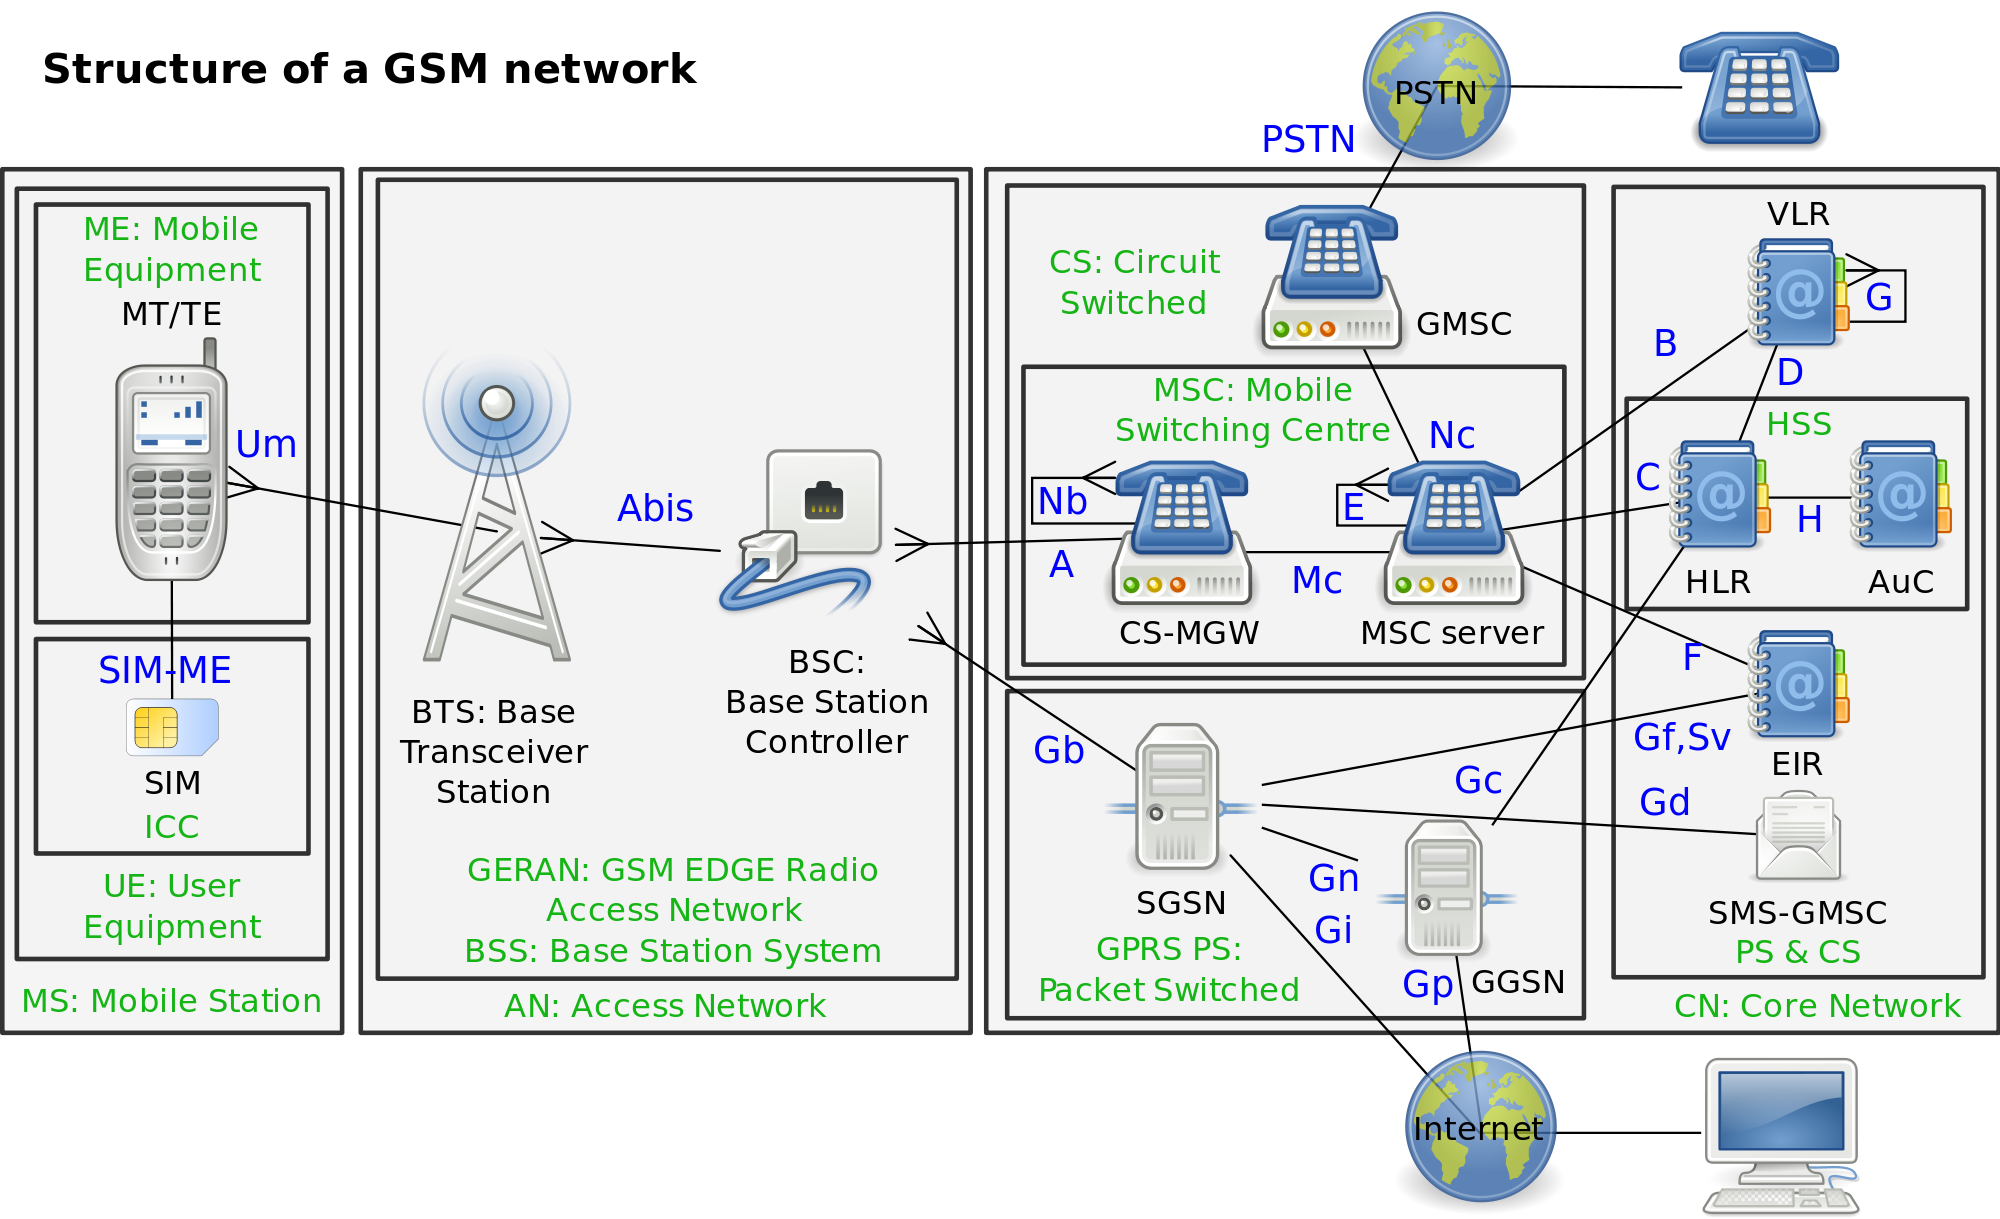
\includegraphics[width=\textwidth]{network_architecture}
    \caption{Key elements of the structure of a GSM
            network~\cite{wikimedia_commons_key_2009}}
    \label{fig:network_architecture}
  \end{figure}

  \section{Core Network entities}

    The \gls{cn} is shown on the right of
    \fref{fig:network_architecture}. It is connected to the \gls{an}, to
    the \gls{pstn} or to the \gls{isdn}, and to the Internet. It is also
    separated between the \gls{cs} domain and the \gls{ps} domain. These
    two domains are overlapping since they contain some common entities,
    but they differ by the way they support user traffic. Basically, the
    entities specific to the \gls{ps} domain are the \gls{gprs} specific
    entities. This section reviews all the relevant \gls{cn} entities in
    turn, and then shortly describes the signaling system used between
    them~\cite{3gpp_ts_2015}.

    \subsection{Home Subscriber Server}

      The \gls{hss} is the entity containing the subscription-related
      information to support the network entities actually handling
      calls or sessions. It is common to the \gls{cs} and \gls{ps}
      domains and contains two different entities: the \gls{hlr} and the
      \gls{auc}~\cite{3gpp_ts_2015}.

      The \gls{hlr} is a database providing a known, fixed location to
      dispense information about an inherently mobile subscriber. It
      stores subscriber information, like the \gls{imsi} and the
      \gls{msisdn}. It also stores location information allowing
      incoming calls to be routed. The \gls{auc} is associated with an
      \gls{hlr} and stores the authentication key Ki for each mobile
      subscriber registered with the associated \gls{hlr}. This key is a
      shared secret between the \gls{auc} and the \gls{sim} and should
      not leave these two entities. It is used with the A3 and A8
      algorithms to generate security data needed for authentication and
      ciphering for each mobile subscriber, for example the session key.
      The \gls{hlr} requests this data from the \gls{auc}, stores it and
      delivers it to the \gls{vlr} and
      \gls{sgsn}~\cite{etsi_gsm_1992,etsi_gsm_2001,3gpp_ts_2015}.

      The \gls{imsi} is a unique number identifying a subscriber on the
      \gls{plmn} and its structure is shown on
      \fref{fig:structure_of_imsi}. It is composed of the \gls{mcc}, the
      \gls{mnc}, and the \gls{msin}. The \gls{mcc} identifies the
      country of origin of the subscriber, the \gls{mnc} identifies the
      home \gls{plmn} of the subscriber within this country, and the
      \gls{msin} identifies the subscriber within this \gls{plmn}. The
      \gls{msisdn} is the phone number of the
      subscriber~\cite{3gpp_ts_2003}.

      \begin{figure}[h]
        \centering
        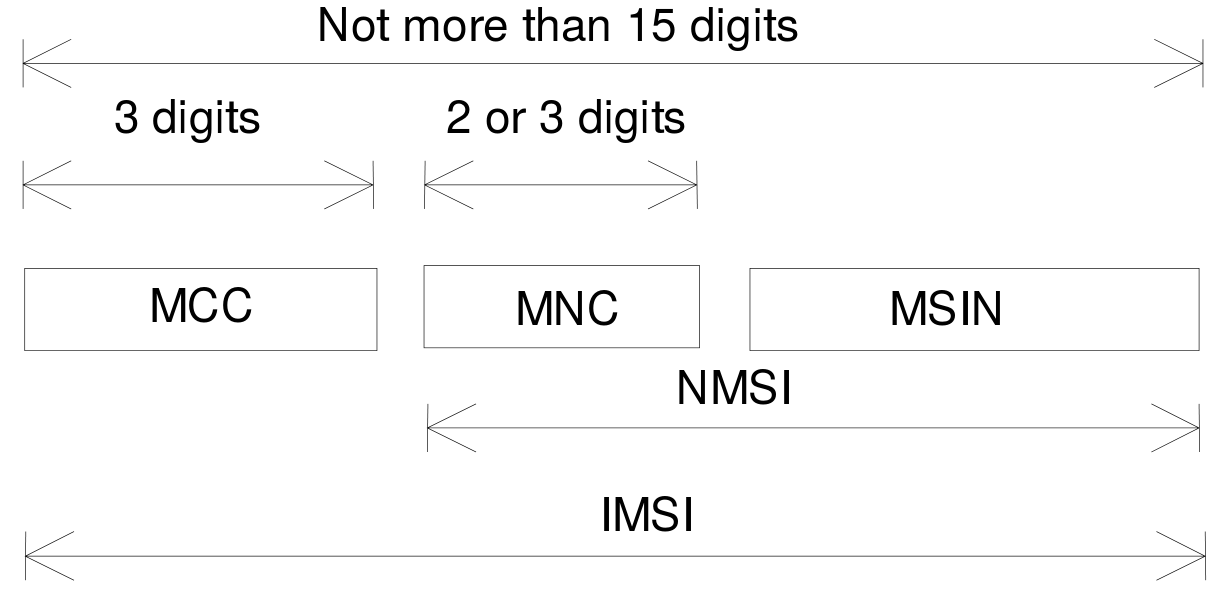
\includegraphics[width=0.7\textwidth]{structure_of_imsi}
        \caption{Structure of an IMSI~\cite{3gpp_ts_2003}}
        \label{fig:structure_of_imsi}
      \end{figure}

    \subsection{Visitor Location Register}

      The \gls{vlr} stores information needed to manage the mobile
      nature of subscribers, when they are located in the \gls{vlr}
      area. It stores identity information, like the \gls{tmsi}, or
      location information, like the \gls{lai} in which the mobile has
      been registered. The \gls{vlr} retrieves information from the
      \gls{hlr} and provides a local storage which is needed to handle
      calls to and from subscribers in the location areas related to the
      \gls{vlr}. The \gls{vlr} is common to the \gls{cs} and \gls{ps}
      domains.

      The \gls{vlr} area is the part of the network controlled by a
      \gls{vlr}. It may consist of one or several \gls{msc} areas. The
      \gls{tmsi} is a temporary number identifying the subscriber
      inside a \gls{vlr} area or inside an \gls{sgsn} area. The
      \gls{la} is defined as an area in which an \gls{ms} may move
      freely without updating the \gls{vlr}. An \gls{lai} is a number
      identifying a location area, and is composed of the \gls{mcc},
      the \gls{mnc}, and the \gls{lac}. This is shown on
      \fref{fig:structure_of_lai}. The \gls{lac} is a number
      identifying a location area within a \gls{plmn}
      ~\cite{etsi_gsm_1992-1,etsi_gsm_2001,3gpp_ts_2003,3gpp_ts_2015}.

      \begin{figure}[h]
        \centering
        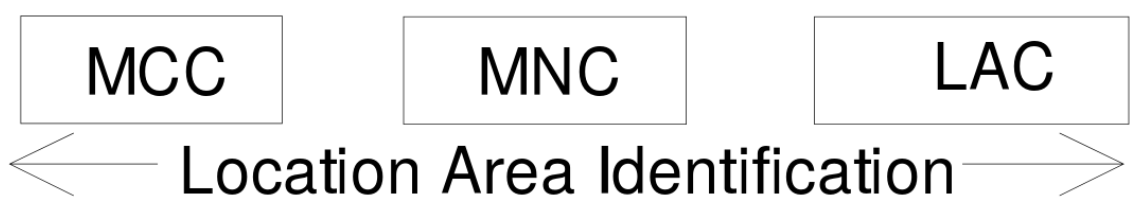
\includegraphics[width=0.5\textwidth]{structure_of_lai}
        \caption{Structure of an \gls{lai}~\cite{3gpp_ts_2003}}
        \label{fig:structure_of_lai}
      \end{figure}

      \iffalse
      GSM 03.08
      0104 def and 0302 full def
      0301. 0303 for tmsi structure
      0308
      \fi

    \subsection{Mobile-services Switching Centre}
    \label{sssection:msc}

      The \gls{msc} constitutes the interface between the radio system
      and the fixed networks. It performs all necessary functions in
      order to handle the circuit switched services to and from the
      \gls{ms}. The \gls{msc} area is the part of the network covered by
      an \gls{msc}. It may consist of one or several location areas, or
      of one or several \gls{bsc} areas.

      The \gls{gmsc} is a specialized \gls{msc}. If a network delivering
      a call to the \gls{plmn} can not interrogate the relevant
      \gls{hlr}, the call is routed to a \gls{gmsc}. This \gls{gmsc}
      will interrogate the appropriate \gls{hlr} and then route the call
      to the \gls{msc} where the \gls{ms} is located. Another
      specialized \gls{msc} is the \gls{sms-gmsc}, which allows
      \gls{sms} messages to be delivered to the \gls{ms}. While the
      \gls{gmsc} is part of the \gls{cs}, the \gls{sms-gmsc} is a common
      entity of the \gls{cs} and \gls{ps} domains~\cite{3gpp_ts_2015}. 

    \subsection{GPRS Support Nodes}

      There are two types of \gls{gsn}: the \gls{ggsn}, and the
      \gls{sgsn}. They constitute the interface between the radio
      system and the fixed networks for packet switched services.
      Together, they perform all necessary functions in order to
      handle the packet transmission to and from the \gls{ms}. The
      \gls{sgsn} area is the part of the network served by an
      \gls{sgsn}. It may consist of one or several routing areas, or
      of one or several \gls{bsc} areas. The \gls{ra} is defined as an
      area in which an \gls{ms} may move freely without updating the
      \gls{sgsn}.

      The \gls{sgsn} has a location register function which stores two
      types of subscriber data needed to handle originating and
      terminating packet data transfer: subscription information,
      including temporary identities, and location information. The
      location register function in the \gls{ggsn} stores subscriber
      data received from the \gls{hlr} and the \gls{sgsn}. It stores
      subscription information, and the address of the \gls{sgsn}
      related to the subscriber~\cite{3gpp_ts_2015}.

    \subsection{MAP protocol of the SS7} 
    \label{sec:ss7}
      
      The \gls{ss7} is used to transfer information between entities of
      the \gls{plmn}, and between \glspl{plmn} and other telephony
      networks. The application level of the \gls{ss7} contains the
      \gls{map} protocol. The \gls{map} is specific to mobile networks,
      and defines various services used to transfer information between
      the entities of the \gls{plmn} defined earlier in this section.
      Three of these services are important for this thesis, and they
      are introduced in this section~\cite{3gpp_ts_2015-2}.

      \subsubsection{MAP-SEND-ROUTING-INFO-FOR-SM}
      \label{sec:sriforsm}

        The MAP-SEND-ROUTING-INFO-FOR-SM service is \textquote{used
        between the gateway MSC and the HLR to retrieve the routing
      information needed for routing the short message to the servicing
    MSC}. This service allows, using a phone number (\gls{msisdn}), to
    request the \gls{imsi} of the related subscriber, as well as the
    number of the \gls{msc} which is serving it. The use of this service
    is illustrated
    on~\fref{fig:map_srifs}~\cite[p.~232]{3gpp_ts_2015-2}.
        
        \begin{enumerate}[topsep=-1em,parsep=0em,itemsep=0em]

          \item The Service Center serving the sending \gls{ms} sends
            the \gls{sms} message to the related \gls{gmsc}.         

          \item This \gls{gmsc} sends a MAP-SEND-ROUTING-INFO-FOR-SM
            request containing the receiving phone number to the
            \gls{hlr} related to that subscriber.

          \item This \gls{hlr} answers with the \gls{imsi} of the
            receiving subscriber, as well as the number of the \gls{msc}
            serving it.

          \item The \gls{gmsc} serving the sender transmits the
            \gls{sms} message to the \gls{msc} serving the receiver.
        
        \end{enumerate}
        
        \begin{figure}[h]
          \centering
          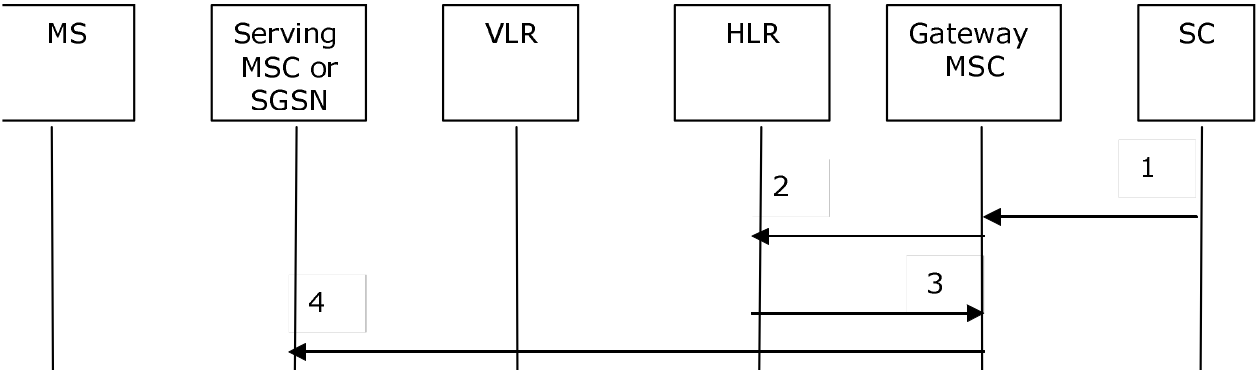
\includegraphics[width=\textwidth]{map_srifs}
          \caption{Beginning of the mobile terminated SMS
          procedure~\cite[p.~792]{3gpp_ts_2015-2}}
          \label{fig:map_srifs}
        \end{figure}

      \subsubsection{MAP-PROVIDE-SUBSCRIBER-Info}
      \label{sec:psi}
          
        The MAP-PROVIDE-SUBSCRIBER-Info service is \textquote{used to
        request information (e.g. subscriber state and location) from
      the VLR or the SGSN at any time}. This service allows, using the
      \gls{imsi} of the subscriber, to request the \gls{cgi} related to
      the phone. An example of this service usage is illustrated
      on~\fref{fig:map_psi}~\cite[p.~181]{3gpp_ts_2015-2}.

        \begin{enumerate}[topsep=-1em,parsep=0em,itemsep=0em]

          \item To establish a call from one \gls{plmn} to another, the
            \gls{msc} of the first network, the VMSC, needs to contact
            the \gls{gmsc} of the second network.

          \item This \gls{gmsc} will contact the \gls{hlr} to request
            the needed routing information.

          \item The \gls{hlr} will then send a
            MAP-PROVIDE-SUBSCRIBER-Info request containing the
            \gls{imsi} of the receiving subscriber.

          \item The \gls{vlr} will answer with the necessary routing
            information, for example the \gls{cgi} of the cell to which
            the receiving subscriber is camping.

        \end{enumerate}

        \begin{figure}[h]
          \centering
          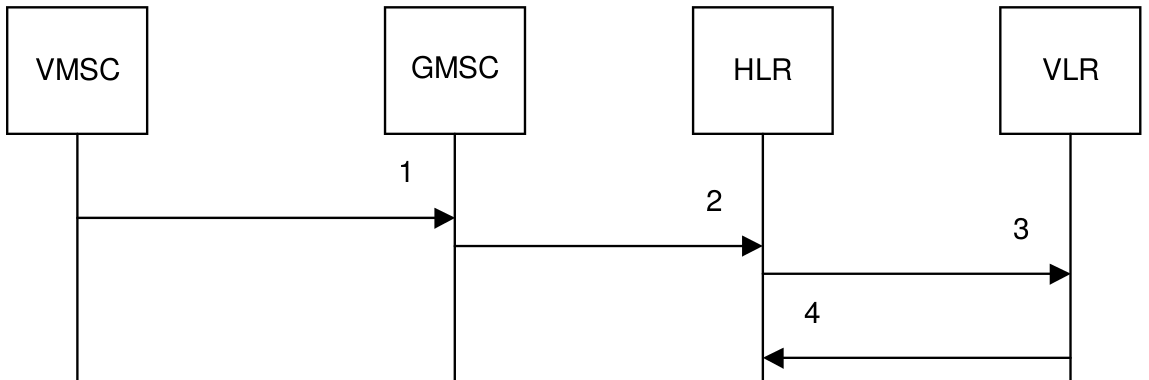
\includegraphics[width=\textwidth]{map_psi}
          \caption{Beginning of the message flow for retrieval of
            routing information~\cite[p.~639]{3gpp_ts_2015-2}}
          \label{fig:map_psi}
        \end{figure}

      \subsubsection{MAP\_SEND\_IDENTIFICATION}
      \label{sec:si}

       The MAP\_SEND\_IDENTIFICATION service \textquote{is used
       between a VLR and a previous VLR to retrieve IMSI and
     authentication data for a subscriber registering afresh in that
   VLR}. This service allows, using the \gls{tmsi} of the phone, to
   request up to five authentication sets, as long as they are
   available. The authentication sets contain information used to
   authenticate the subscriber and to encrypt its communications on the
   Um interface. An example of this service usage is illustrated
   on~\fref{fig:map_si}~\cite[p.~118]{3gpp_ts_2015-2}.

        \begin{enumerate}[topsep=-1em,parsep=0em,itemsep=0em]

          \item When an \gls{ms} wants to send its location to the
            network, it sends a Location Update request message.         

          \item The related \gls{vlr} will then send a
            MAP\_SEND\_IDENTIFICATION request containing the \gls{tmsi}
            of the subscriber to the Previous \gls{vlr}.

          \item This Previous \gls{vlr} will answer to the new \gls{vlr}
            with a response message containing the \gls{imsi} of the
            subscriber, as well as the related authentication sets.

        \end{enumerate}

        \begin{figure}[h]
          \centering
          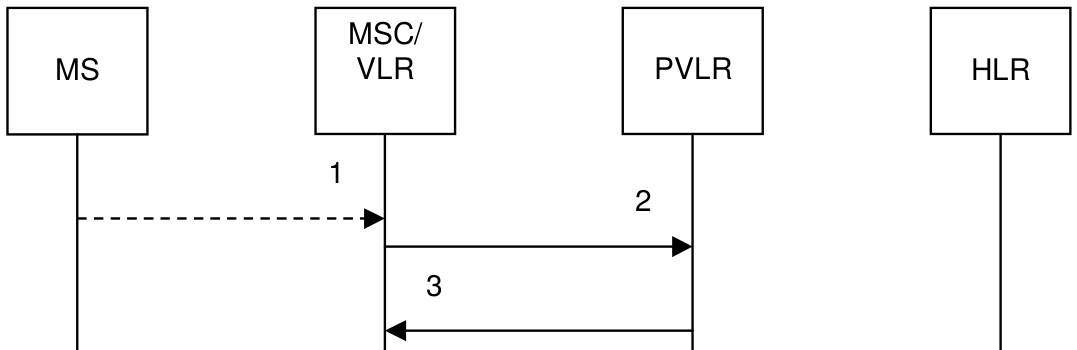
\includegraphics[width=\textwidth]{map_si}
          \caption{Beginning of the message flow for location updating
          to a new VLR area, when the IMSI can be retrieved from the
          previous VLR~\cite[p.~479]{3gpp_ts_2015-2}}
          \label{fig:map_si}
        \end{figure}
      
  \section{Access Network entities}

    After having introduced the \gls{cn} and its entities, this section
    focuses on the \gls{geran}, also called the \gls{bss}, which is
    shown in the middle of \fref{fig:network_architecture}. It is the
    system of base station equipments which is viewed by the \gls{msc}
    as being the entity responsible for communicating with \glspl{ms} in
    a certain area. A \gls{bss} is subdivided into a control function
    carried out by the \gls{bsc} and a radio transmitting function
    carried out by the \gls{bts} with its transceivers, TRX. In order to
    keep the \gls{bts} as simple as possible, it contains only those
    functions which have to reside close to the radio
    interface~\cite{etsi_gsm_2001,3gpp_ts_2002,3gpp_ts_2015}.

    \subsection{Base Station Controller}

      A \gls{bsc} is a network component in the \gls{plmn} with the
      function to control one or more \glspl{bts}. The \gls{bsc} area
      is an area of radio coverage consisting of one or more cells
      controlled by one \gls{bsc}, which is responsible for most of
      the functions of the
      \gls{bss}~\cite{etsi_gsm_2001,3gpp_ts_2002,3gpp_ts_2015}.
 
    \subsection{Base Transceiver Station}
    \label{sec:cgi}

      A \gls{bts} is a network component which serves one cell, and is
      controlled by a \gls{bsc}. Among other things, it is responsible
      for power and time measurements, and \gls{rach} detection. It
      then sends that information back to the \gls{bsc} for analysis.
      It is also responsible for error protection coding and decoding,
      and encryption~\cite{etsi_gsm_2001,3gpp_ts_2002,3gpp_ts_2015}.
    
      \iffalse
      The cell is an area of radio coverage
      identified by a Base station identification\fxnote{defref}.
      0303
      \fi

      A cell is identified by a \gls{cgi} number, as shown on
      \fref{fig:structure_of_cgi}. It is composed of the \gls{mcc},
      the \gls{mnc}, the \gls{lac}, and the \gls{ci}. The \gls{ci}
      identifies the cell within a \gls{plmn}.

      \begin{figure}[h]
        \centering
        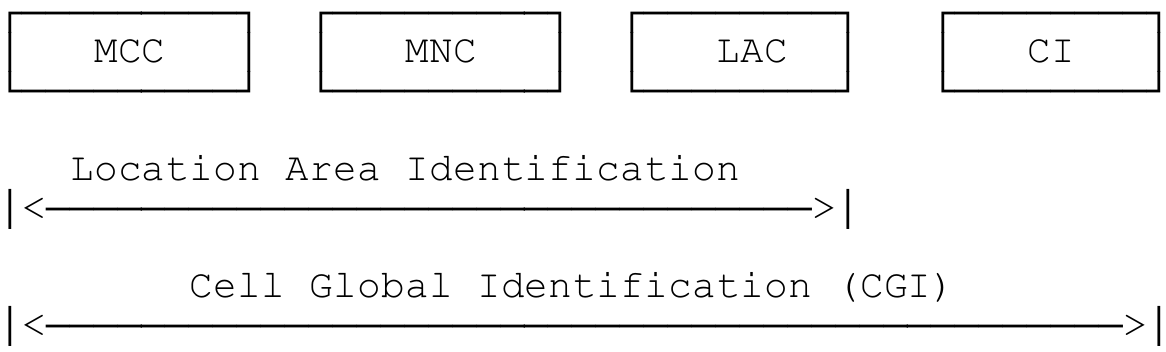
\includegraphics[width=0.7\textwidth]{structure_of_cgi.png}
        \caption{Structure of Cell Global
        Identification~\cite[p.~14]{3gpp_ts_2003}}
        \label{fig:structure_of_cgi}
      \end{figure}


    \section{Mobile Station}

      Finally, the last element of the \gls{plmn} infrastructure is the
      \gls{ms} or \gls{ue}. It consists of the physical equipment used
      by a \gls{plmn} subscriber and is shown on the left of
      \fref{fig:network_architecture}. It comprises the \gls{me} and the
      \gls{sim}. The \gls{me} is the mobile phone itself and contains
      the \gls{imei}, a unique number identifying the equipment, while
      the \gls{sim} is a removable module containing the \gls{imsi}, a
      unique number identifying a subscriber. Like the \gls{auc}, the
      \gls{sim} also stores the subscriber authentication key Ki, can
      execute the A3 algorithm for authentication, and the A8 algorithm
      to generate a session key Kc. The A5 algorithm is executed on the
      \gls{me} to encrypt the communications on the Um interface.
      Finally, the \gls{sim} also stores temporary network data, like
      the
      \gls{tmsi}~\cite{etsi_gsm_2000,etsi_gsm_2001,3gpp_ts_2014-1,3gpp_ts_2015}.

\chapter{Protocol stack implementation}
\label{chap:protocol_stack_implementation}

This chapter is dedicated to the \proj{OsmocomBB} implementation of the
\gls{gsm} \gls{ms} protocol stack. It is meant to serve as a small guide
into the source code by providing an overview of its inner workings, as
well as references to the available documentation. The information is
directly extracted from the \gls{3gpp} specifications, from the source
code, and from the project wiki. Since it would be impossible to cover
every aspect of this protocol stack in one chapter, it only provides
information relevant for the other chapters of this thesis. For more
information, refer to the specifications
directly~\cite{3gpp_specifications_????,osmocombb_ms-side_????,osmocombb_2015}.

%3GPP TS 44.001 version 12.0.0 Release 12 9 {
As explained in~\Cref{chap:network_architecture}, the \gls{ms} is
connected to the network through the Um interface, or air interface. The
protocols on this interface are separated in three layers: the physical
layer, or layer 1, the data link layer, or layer 2, and the layer 3.
Each will be investigated in turn in the following
sections~\cite{3gpp_ts_2014-2}.
%}

\section{Physical layer}

  %3GPP TS 44.004 version 12.0.0 Release 12 8 {
  The first layer of the \gls{gsm} \gls{ms} protocol stack is the
  physical layer, which provides logical channels for the upper layers.
  There are two types of logical channels: channels dedicated to
  signaling data, and channels dedicated to voice traffic. The
  establishment, release, and control of the signaling channels is
  supervised by the \gls{rr} sublayer of the layer 3, based on
  measurements from layer 1. This allows the \gls{ms} to select the best
  cell, but also to adapt the various parameters when a signaling
  channel is established. These channels are used by layer 2 to transmit
  an error protected and encrypted bit stream over the radio medium. The
  control of the channels dedicated to voice traffic is left to other
  functional units. The interfaces of the physical layer are shown
  on~\fref{fig:l1_interfaces}~\cite{3gpp_ts_2014-4}.

    \begin{figure}[h]
      %GSM 04.04 version 5.0.1: April 1997 Page 9
      \centering
      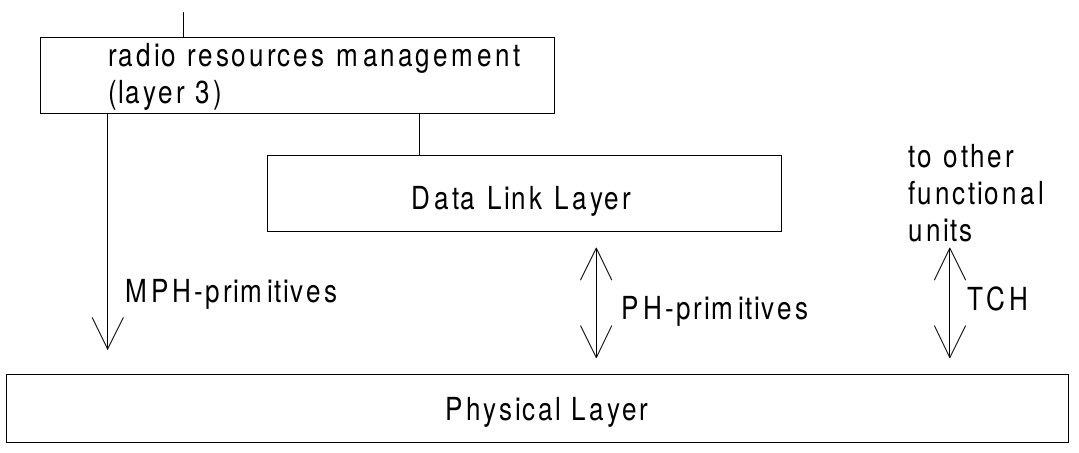
\includegraphics[width=0.7\textwidth]{l1_interfaces}
      \caption{Interfaces with the physical layer~\cite{etsi_gsm_1997}}
      \label{fig:l1_interfaces}
    \end{figure}

  \subsection{Channels}

    This section will first introduce the various logical channels and
    their roles. Then, it will define the physical channels, and
    describe how they are created from multiplexing in the frequency and
    time domains. Finally, it will detail the mapping of the logical
    channels on the physical channels.

    \subsubsection{Logical channels}

      %3GPP TS 44.003 version 12.0.0 Release 12 {
      %and a very little bit of 3GPP TS 45.002 version 12.4.0 Release 12 

      The physical layer offers a transmission service on a limited set
      of logical channels. As already stated, these logical channels are
      of two types: the traffic channels and the control channels.
      Traffic channels are intended to carry encoded speech, while the
      control channels are intended to carry signaling information for
      the layer 3 entities. These two channels can be subdivided in
      subcategories again as shown
      on~\tref{tab:logical_channels}~\cite{3gpp_ts_2014-3,3gpp_ts_2015-4}.

       \begin{table}[h]
          \centering
          \begin{tabular}{@{}lll@{}}
            \toprule
            Type          & Name                    \\
            \midrule

            \multirow{2}{*}{\parbox{0.30\textwidth}{\raggedright Traffic
            Channel (TCH)}} & Full-rate or Bm (TCH/F) \\
                          & Half-rate or Lm (TCH/H) \\

            \\

            \multirow{3}{*}{\parbox{0.30\textwidth}{\raggedright Broadcast
            Channel}} & Frequency Correction Channel (FCCH)\\
                          & Synchronization Channel (SCH)\\
                          & Broadcast Control Channel (BCCH)\\
            \\

            \multirow{3}{*}{\parbox{0.30\textwidth}{\raggedright Common
            Control Channel (CCCH)}} & Random Access Channel (RACH)\\
                          & Access Grant Channel (AGCH)\\
                          & Paging Channel (PCH)\\
            \\
             \multirow{3}{*}{\parbox{0.30\textwidth}{\raggedright
             Dedicated Control Channel (DCCH)}} & Standalone Dedicated Control Channel (SDCCH)\\
                          & Slow Associated Control Channel (SACCH)\\
                          & Fast Associated Control Channel (FACCH)\\
            \bottomrule
          \end{tabular}
          \caption{Logical channels~\cite{3gpp_ts_2015-3}}
          \label{tab:logical_channels}
        \end{table}

      \glspl{tch} can be divided in two categories depending on their
      bit rate capacity: Bm or Full-rate (TCH/F), and Lm or Half-rate
      (TCH/H). Control channels are divided in three subcategories
      depending on their roles: the Broadcast Control channels, the
      \gls{ccch}, and the \gls{dcch}. Each of these can be subdivided
      again.

      The Broadcast Control channels are subdivided into three other
      channels. The \gls{bcch} intended to broadcast a variety of
      information, including information necessary for an \gls{ms} to
      register in the system. The \gls{fcch}, intended for frequency
      correction. And the \gls{sch}, intended for frame synchronization
      and identification of a \gls{bts}.

      The \gls{ccch} is subdivided in three other channels. The
      \gls{rach}, which is the only part of the \gls{ccch} used to
      transmit information from the \gls{ms} to the network. The
      \gls{agch}, which is the part reserved for assignment messages.
      And the \gls{pch}, which is used in the paging process.

      Finally, the \gls{dcch} is subdivided into three channels. The
      \gls{sdcch}, which is a bi-directional \gls{dcch} whose allocation
      is not linked to the allocation of a \gls{tch}. The \gls{facch},
      which is a bi-directional \gls{dcch} obtained by stealing bursts
      from its associated traffic channel. The allocation of a
      \gls{facch} is obviously linked to the allocation of a \gls{tch}.
      And the \gls{sacch}, which is a bi-directional or uni-directional
      \gls{dcch}. An independent \gls{sacch} is always allocated
      together with a \gls{tch} or an \gls{sdcch}.
      %}

    \subsubsection{Physical channels}

      %3GPP TS 45.001 version 12.1.0 Release 12
      %3GPP TS 45.002 version 12.4.0 Release 12 {

      The logical channels mentioned above are mapped on physical
      channels that are described in this section. The complete
      definition of a particular physical channel consists of a
      description in the frequency domain, and a description in the time
      domain~\cite{3gpp_ts_2015-3,3gpp_ts_2015-4}.

      In the frequency domain, the radio spectrum is first divided into
      frequency bands. Each of these bands is then separated between two
      groups, the uplink frequencies, where the mobile transmits and the
      network receives, and the downlink frequencies, where the network
      transmits and the mobile receives. This is the \gls{fdd} scheme.
      Finally, the carrier frequencies are grouped by pair, comprised of
      one carrier frequency in the upper band and one carrier frequency
      in the lower band, to form an \gls{arfcn}. This is the \gls{fdma}
      scheme. Each cell is allocated a subset of these \glspl{arfcn},
      and one of them is used as the beacon channel.

      In the time domain, the access scheme is \gls{tdma} with eight
      basic physical channels per carrier. The basic radio resource is a
      time slot lasting approximately \SI{576.9}{\micro\second}. The
      \gls{gsm} system uses the \gls{gmsk} modulation with a modulation
      rate of around \SI{270.833}{\kilo symbol\per\second}. This means
      that the time slot duration, including guard time, is
      \SI{156.25}{symbols} long. At the \gls{bts} the start of a
      \gls{tdma} frame on the uplink is delayed by the fixed period of 3
      time slots from the start of the \gls{tdma} frame on the downlink.
      This allows the same time slot number to be used in the downlink
      and uplink whilst avoiding the requirement for the \gls{ms} to
      transmit and receive simultaneously. This can be seen
      in~\fref{fig:l1_3ts_hop}.

      \begin{figure}[h]
        \centering
        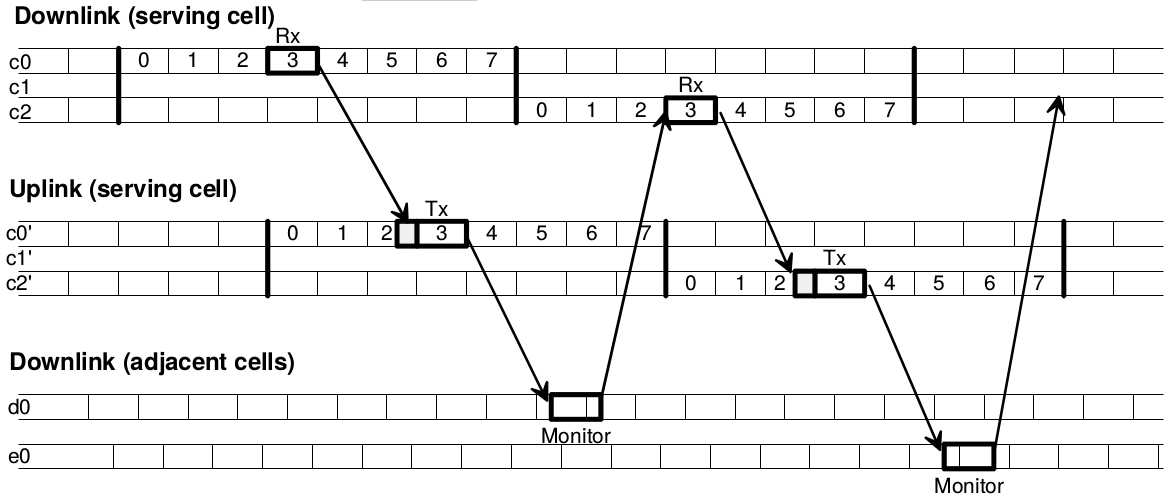
\includegraphics[width=\textwidth]{l1_3ts_hop}
        \caption{Uplink delay and frequency hopping~\cite{3gpp_ts_2015-4}}
        \label{fig:l1_3ts_hop}
      \end{figure}

      The physical content of a time slot is represented by a burst. It
      is defined as a period of a carrier which is modulated by a data
      stream. For the \gls{gmsk} modulation, a symbol represents one bit,
      and thus a burst contains \SI{156.25}{bits}. The period between
      bursts appearing in successive time slots is called the guard
      period and explains the fractional component in the amount of
      bits. Different types of bursts exist in the system, and they are
      displayed on~\fref{fig:bursts}.

      \begin{figure}[h]
        \centering
        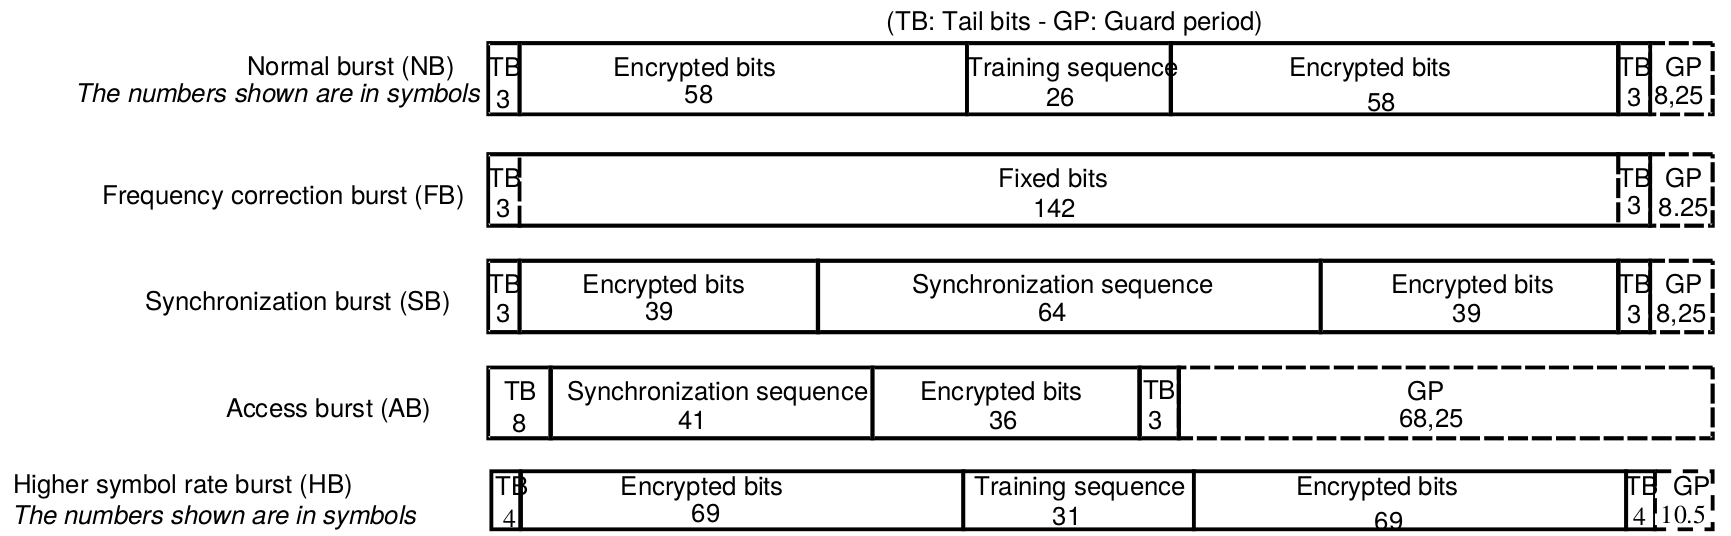
\includegraphics[width=\textwidth]{bursts}
        \caption{Types of bursts~\cite{3gpp_ts_2015-3}}
        \label{fig:bursts}
      \end{figure}

      The frequency hopping capability is optionally used to reduce the
      noise on the communication and is displayed
      on~\fref{fig:l1_3ts_hop}. The principle is that every \gls{ms}
      switches between frequencies according to a given sequence. It
      transmits or receives during one time slot on a fixed frequency
      and must hop on the following before the same time slot on the
      next \gls{tdma} frame. It must be noted that on the beacon
      channel, frequency hopping is not permitted on any time slot
      supporting a \gls{bcch}.
      %}

    \subsubsection{Mapping of the logical channels}

      %3GPP TS 45.001 version 12.1.0 Release 12
      %3GPP TS 45.002 version 12.4.0 Release 12 {

      The \gls{tdma} frames described in the previous section are
      grouped in multiframes. Two types of multiframes exist in the
      system: 26-multiframes comprising 26 \gls{tdma} frames which are
      used to carry traffic channels, and 51-multiframes comprising 51
      \gls{tdma} frames, used to carry signaling channels. These
      multiframes are organized respectively by groups of 51 or 26 to
      form superframes, which are the least common multiple of the time
      frame structures. Finally, 2048 superframes are grouped in
      hyperframes which form the longest recurrent time
      period~\cite{3gpp_ts_2015-3,3gpp_ts_2015-4}.

      \iffalse
      This is shown in~\fref{fig:frames}.
      \begin{figure}[h]
        \centering
        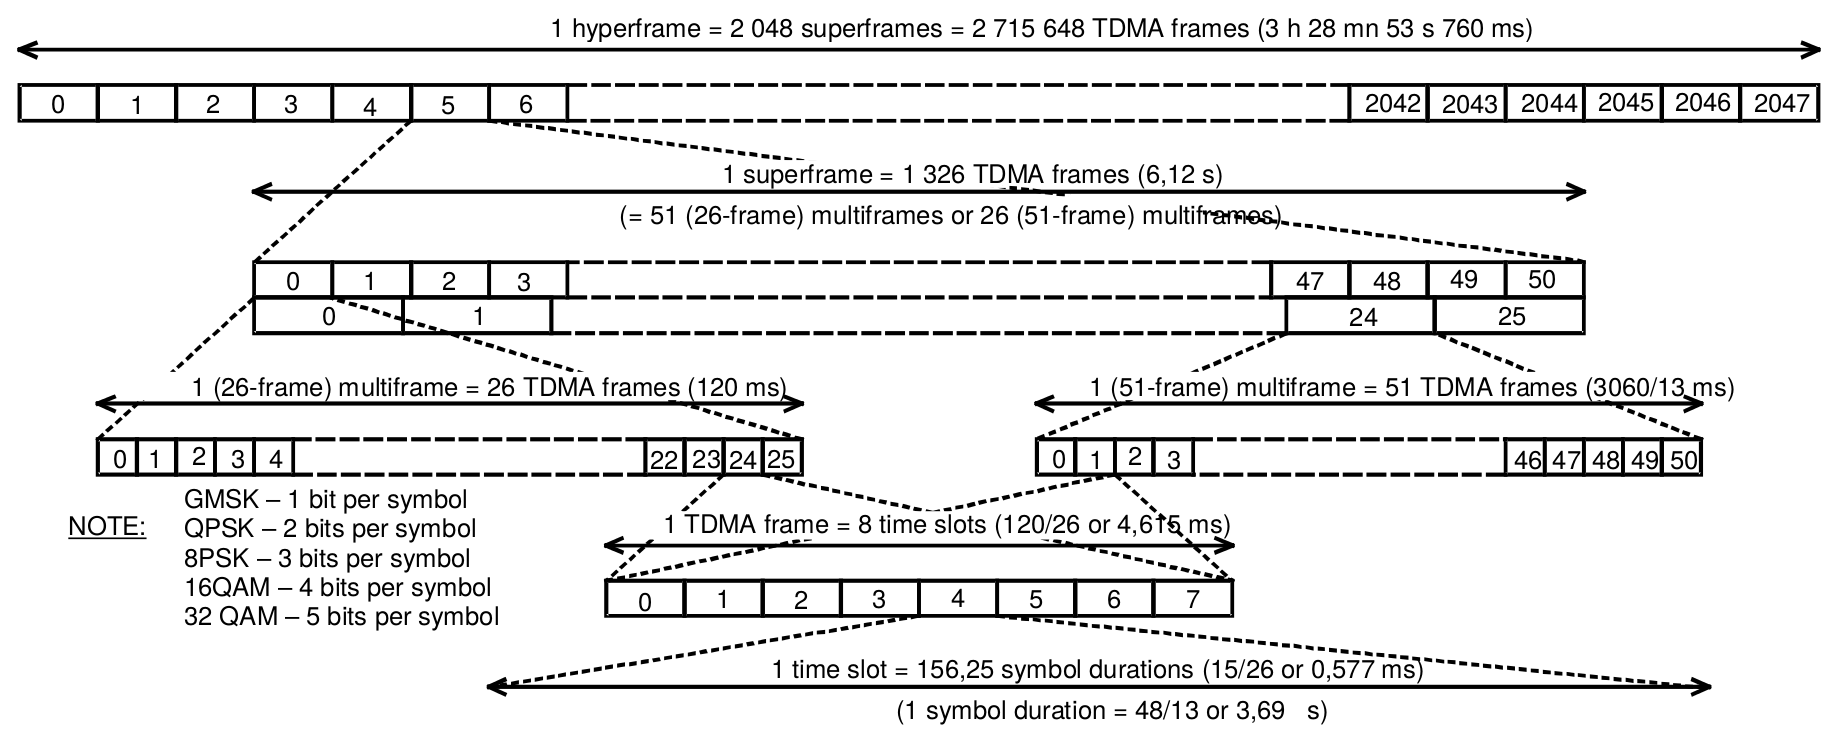
\includegraphics[width=\textwidth]{frames}
        \caption{Logical channels on the 51-multiframe
        ~\cite{3gpp_ts_2015-3}}
        \label{fig:frames}
      \end{figure}
      \fi

      The logical channels are defined by mapping the multiframes on the
      physical channels. For example, on the physical channel composed
      of the time slot $0$ on the beacon frequency, there is a
      $51$-multiframe containing logical channels.
      On~\fref{fig:51multiframe_b-c}, the letter F represents the
      \gls{fcch}, the letter S represents the \gls{sch}, the letter B
      represents the \gls{bcch}, and the letter C represents the
      \gls{ccch}. The \gls{fcch} can be found on time slot $0$ of the
      \gls{tdma} frames $1$, $11$, $21$, $31$, and $41$ of the
      multiframe. This is a kind of \gls{tdma} inside a \gls{tdma}.

      \begin{figure}[h]
        \centering
        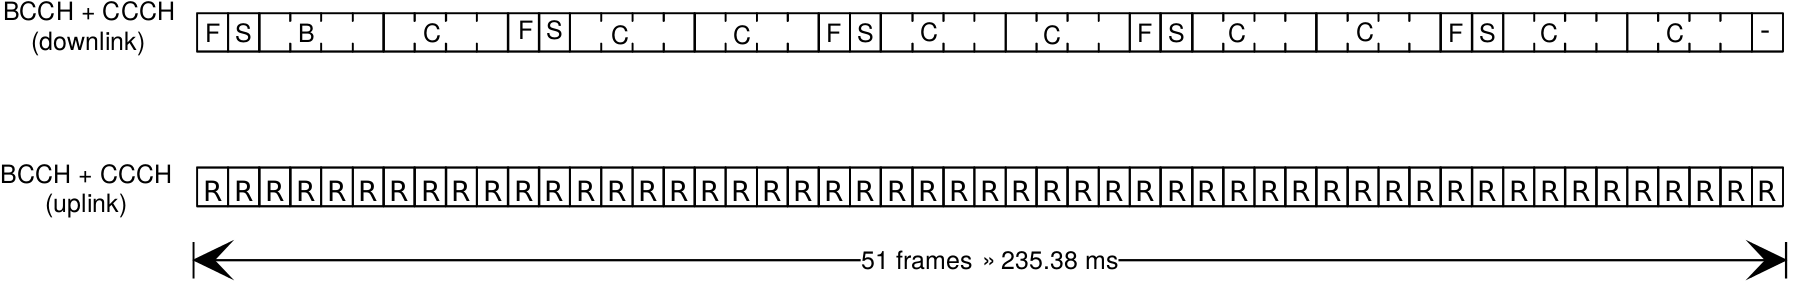
\includegraphics[width=\textwidth]{51multiframe_b-c}
        \caption{3GPP TS 45.001 version 12.1.0 Release 12 20}
        \label{fig:51multiframe_b-c}
      \end{figure}
      %}

  \subsection{Modem}
  \label{sec:modem}
    %3GPP TS 45.001 version 12.1.0 Release 12 {
    %\url{http://bb.osmocom.org/trac/wiki/Rita}
    %~\cite{osmocombb_2015,welte_anatomy_2010}

    The previous section focused on the channels handled by the physical
    layer, and this section will focus on the bitstream transmitted on
    the radio medium. The physical layer is responsible for converting
    the \gls{rf} signals in bursts, and the bursts to packets that can
    be handled by the data link layer. Of course, it is also responsible
    for the inverse operation~\cite{3gpp_ts_2015-3,osmocombb_2015,welte_anatomy_2010}.

    The physical layer is highly dependent on the hardware, and it is
    therefore interesting to take a look at the platform supported by
    the \proj{OsmocomBB} project. This platform is the \gls{ti} Calypso
    based modem from which a block schematic is represented
    on~\fref{fig:calypso_modem}. The Calypso based modem includes an
    \gls{rf} frontend, an \gls{abb}, and a \gls{dbb}.

    \begin{figure}[h]
      \centering
      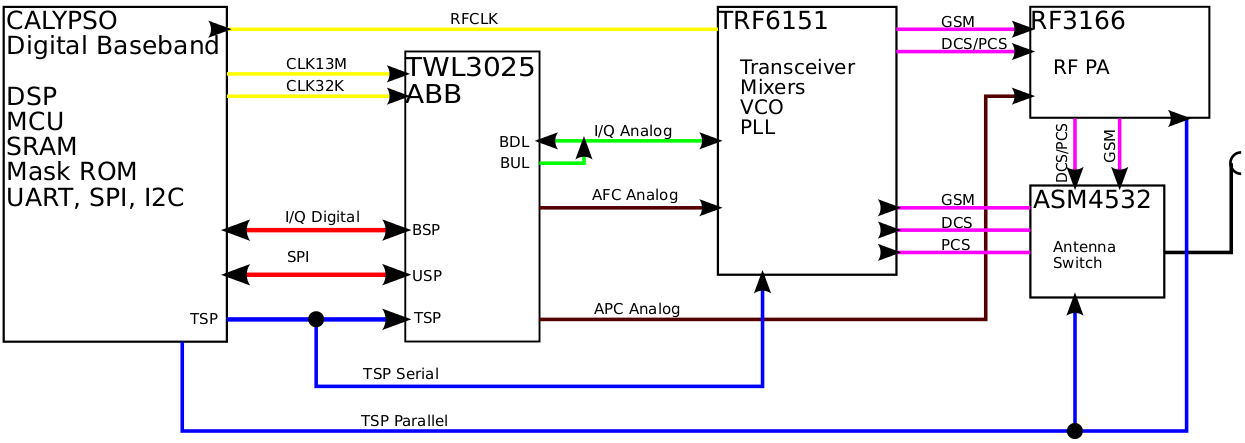
\includegraphics[width=\textwidth]{calypso-block}
      \caption{Block diagram of a typical Calypso based
              modem~\cite{welte_anatomy_2010}}
      \label{fig:calypso_modem}
    \end{figure}

    The \gls{rf} frontend is used to receive and transmit at the GSM
    frequency, and is composed of an antenna switch, an \gls{rf} power
    amplifier controlling the output level, and a \gls{ti} Rita GSM
    transceiver. The antenna switch routes the signal to the receive or
    transmit path. On the receive path, the signal is filtered and
    amplified to prevent noise. Then, it is mixed with a frequency
    generated by the local oscillator and filtered again to convert it
    from the \gls{gsm} frequency to a baseband signal. Finally, this
    baseband signal is sent to the \gls{abb}. On the transmit path, the
    \gls{rf} frontend receives a signal from the \gls{abb}, converts it
    to the relevant \gls{gsm} frequency, sends it to the \gls{rf} power
    amplifier shown on the top right of the schematic, and sends it to
    the antenna switch which now connects the transmit path with the
    antenna.

    The \gls{ti} Iota \gls{abb} deals with the sampling, the
    differential encoding, and the modulation. On the receive path, when
    the \gls{abb} receives the analog signal from the \gls{rf} frontend,
    it simply filters and samples it in an \gls{adc}, before sending the
    digital samples to the \gls{dbb}. On the transmit path, the
    \gls{abb} receives digital signals from the \gls{dsp}, modulates
    them and converts them to analog signals in a \gls{dac}. The
    modulation is done in the \gls{abb} because it is much simpler to
    apply a \gls{gmsk} modulation than a demodulation. This reduces the
    complexity of the \gls{dsp}, and therefore its cost and power
    consumption.

    The \gls{ti} Calypso \gls{dbb} on the left is composed of a
    \gls{dsp} and an \comp{ARM7TDMI} processor. The \gls{dsp} is
    responsible for the the demodulation, the burst building and
    multiplexing, the encryption, the interleaving, reordering and
    partitioning, and finally the coding. The \comp{ARM7} processor is
    called the Baseband Processor and runs the \proj{OsmocomBB}
    implementation of the \gls{gsm} \gls{ms} protocol stack.

    \proj{OsmocomBB} implements the drivers for the various components
    of the platform: the \gls{rf} transceiver, the \gls{abb}, or the
    \gls{dsp}, but also the keypad, the display, and so on. For example,
    the \gls{dsp} communicates with the baseband processor using an API
    available through a shared memory interface. \proj{OsmocomBB} does
    not modify the code inside the \gls{dsp}, but drives it by
    implementing this API. Therefore, code running on the baseband
    processor can use the various tasks provided by the \gls{dsp}.

  \subsection{Procedures}
  %3GPP TS 44.004 version 12.0.0 Release 12{
    %3GPP TS 44.005 version 12.0.0 Release 12 5 {

    To provide its various services, the physical layer implements three
    types of procedures. The first ones are the control procedures,
    which handle the control of the various channels. These procedures
    are composed of primitives between the physical layer and the
    \gls{rr} sublayer of the layer 3. The second ones are the interface
    procedures. They are composed of four kind of primitives between the
    physical layer and the data link layer. The first kind is used for
    connection establishment, the second one is used for data
    transmission, the third is used for random access over the
    \gls{rach}, and the last one is used for transmission and
    synchronization. A third type of procedure exists to handle the
    traffic channels~\cite{3gpp_ts_2014-4,3gpp_ts_2014-5,osmocombb_ms-side_????}.
    %}

    All these primitives are implemented in the \proj{OsmocomBB}
    \prog{layer 1} application running on the baseband processor. They
    make use of the hardware detailed in the previous section by using
    the various drivers and the \gls{dsp} API. This application also
    implements the various schedulers needed to use these primitives at
    the right time.

    The layer 1 can be divided in two main parts: the synchronous and
    the asynchronous part. The first one is executed synchronously with
    the \gls{tdma} frame clock thanks to interrupts at every new
    \gls{tdma} frame. The second one uses the data provided by the
    synchronous part and schedules the next actions. It also typically
    communicates with the upper layers, which run on a computer and
    communicate with the layer 1 using the L1CTL interface through a
    serial connection. This interface is implemented in
    \code{src/target/firmware/layer1/l23\_api.c} on the \gls{ms} side,
    and in \code{src/host/layer23/src/common/l1ctl.c} on the computer
    side.

\section{Data link layer}

%3GPP TS 44.005 version 12.0.0 Release 12 5 {
  The data link layer is the second layer of the \gls{gsm} \gls{ms}
  protocol stack. It uses the signaling channels established by the
  physical layer to provide data link connections to the layer 3 by
  implementing a protocol called \gls{lapdm}, where Dm channel is
  another name to designate the signaling channels. This protocol can
  initiate acknowledged or unacknowledged data link connections. The
  first ones implement error recovery procedures and flow control, while
  the second ones do not~\cite{3gpp_ts_2014-5}.   
%}

  \subsection{Procedures}

%3GPP TS 44.005 version 12.0.0 Release 12 5 {
  The data link layer provides two relevant procedures: the random
  access procedure, and the data link procedure. The random access
  procedure is used for data links on the \gls{rach} to format and
  initiate the transmission of the random access frames~\cite{3gpp_ts_2014-5}.

  The data link procedure is used to transmit information between layer
  3 entities across the Um interface. It can handle to types of
  operations: acknowledged and unacknowledged. The first one implements
  error recovery procedures and flow control, and handles numbered
  information frames that are acknowledged by the receiving data link
  layer. It also offers segmentation of layer 3 messages if they do not
  fit in one frame. The second one does not implement any of this and
  handles unnumbered information frames. The \gls{bcch}, the \gls{pch},
  and the \gls{agch} will only support unacknowledged operation, and the
  \gls{dcch} will support both types.
%}

  %http://events.ccc.de/congress/2010/Fahrplan/attachments/1771_osmocombb-27c3.pdf
  %{
  These procedures are performed using three types of primitives. The
  first one is associated with random access, the second one is
  associated with the unacknowledged information transfer service, and
  the last one is associated with the multiple frame acknowledged
  information transfer services. All these primitives are implemented in
  \proj{OsmocomBB} in the \code{src/shared/libosmocore/gsm/lapdm.c} and
  \code{src/shared/libosmocore/gsm/lapd\_core.c} files. Since the data
  link layers are similar on both side of the Um interface, the code
  used in the \proj{OpenBSC} project is reused and extended when
  necessary, and this is why it can be found in the
  \code{src/shared/libosmocore/} directory. The data link layer
  communicates with the physical layer over a serial communication using
  the L1CTL interface. It also communicates with the layer 3 using the
  RSLms interface~\cite{osmocombb_ms-side_????,welte_osmocombb:_2010-1}.
  %}

  \iffalse
  %http://events.ccc.de/congress/2010/Fahrplan/attachments/1771_osmocombb-27c3.pdf {
  interface between Layer2 and Layer3 called RSLms
  In the GSM network, Um Layer2 terminates at the BTS but
  is controlled by the BSC
  Reuse this GSM 08.58 Radio Signalling Link
  Extend it where needed for the MS case
  %}
  \fi

\section{Layer 3}

%3GPP TS 24.007 version 12.0.0 Release 12 22 {
  The last layer of the \gls{gsm} \gls{ms} protocol stack is the layer
  3. It is composed of three sublayers: the \gls{rr} sublayer, the
  \gls{mm} sublayer, and the \gls{cm} sublayer. The \gls{cm} sublayer is
  further divided into functional blocks including the mandatory blocks
  for \gls{ss}, \gls{sms}, and \gls{cc}~\cite{3gpp_ts_2014-6}.

  %} 3GPP TS 44.018 version 12.5.0 Release 12{
  Complete layer 3 transactions consist of specific sequences of
  elementary procedures. Therefore, the following sections will describe
  these procedures for each of the sublayers. The last section will then
  provide an example for a complete \gls{mtc}, which involves all the
  procedures described here.
  
  Since all these procedures are implemented in the \prog{mobile}
  application of \proj{OsmocomBB}, output of this application is
  provided as practical examples. Each line of the logs contains the
  file name, followed by the line number, and the message. For example:
  \code{gsm48\_rr.c:4820 Channel provides data}. This is an easy way to
  find were a given procedure is implemented. The code of this
  application can be found in the \code{src/host/layer23/src/mobile/}
  directory~\cite{3gpp_ts_2015-2,osmocombb_ms-side_????}.
    %}

  \iffalse
  The procedures introduced in this section are placed in context in
  complete examples in \Sref{} and \Sref{}. They are also shown in
  \Sref{}, where the use of the \proj{OsmocomBB} applications is
  demonstrated. 
  \fi

  \subsection{Radio Resource Management procedures}
  \label{sec:rr_proc}

    %3GPP TS 44.018 version 12.5.0 Release 12{
    \gls{rr} procedures include the functions related to the management
    of the control channels and the data link connections on these
    channels. They are implemented in the \prog{mobile} application of
    \proj{OsmocomBB} in the \code{mobile/gsm48\_rr.c} and
    \code{mobile/gsm322.c} file. Their general purpose is to establish,
    maintain and release \gls{rr} connections that allow a dialogue
    between the network and a mobile station. When a connection is
    established, the \gls{rr} sublayer is in dedicated mode. When a
    connection is not established, it is in idle
    mode~\cite{3gpp_ts_2015-2}.

    When in idle mode, the \gls{rr} procedures include the reception and
    measurement of the \gls{bcch} and \gls{ccch}. The measurements are
    coming from the physical layer and are treated to assess the need of
    a cell change. The way it happens in the \prog{mobile} application
    is shown through logs displayed on \fref{fig:pm}, \fref{fig:pm2},
    and \fref{fig:pm3}. The \gls{ms} will first measure the power level
    of all the neighboring cells, then try to synchronize to each of
    them and read their System Information messages, and finally deduce
    the cell reselection parameters. These parameters are used to
    determine if a cell change is needed~\cite{3gpp_ts_2014-8}.

      \begin{figure}
        \centering
        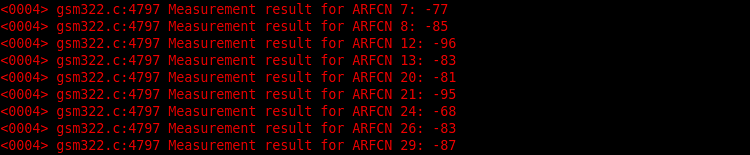
\includegraphics[width=\textwidth]{pm}
        \caption{Power measurements logs in \prog{mobile}: signal
        strength}
        \label{fig:pm}
      \end{figure}

      \begin{figure}
        \centering
        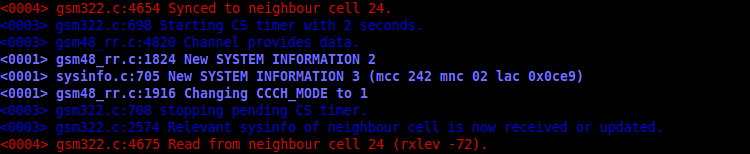
\includegraphics[width=\textwidth]{pm2}
        \caption{Power measurements logs in \prog{mobile}: System
        Information messages}
        \label{fig:pm2}
      \end{figure}

      \begin{figure}
        \centering
        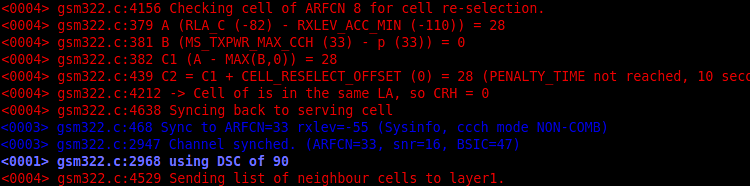
\includegraphics[width=\textwidth]{pm3}
        \caption{Power measurements logs in \prog{mobile}: reselection
        parameters}
        \label{fig:pm3}
      \end{figure}

    To switch from idle mode to dedicated mode, an immediate assignment
    procedure can be initiated by the \gls{rr} sublayer of the \gls{ms}
    in two cases. Firstly, upon reception of a request from the \gls{mm}
    sublayer to enter the dedicated mode. Secondly, in response to a
    Paging Request message assigned to its \gls{tmsi} or \gls{imsi}, and
    received when listening to the \gls{ccch}. In these cases, the
    \gls{rr} sublayer schedules the sending on the \gls{rach} of a
    Channel Request message containing an establishment cause and a
    random reference. Then, it waits until reception of an Immediate
    Assignment message, which contains information regarding the
    \gls{dcch} assigned to the \gls{ms}. If it receives an Immediate
    Assignment Reject or if it does not receive any message after the
    maximum amount of Channel Request messages have been sent, the
    \gls{rr} sublayer aborts the procedure. A successful immediate
    assignment procedure in the \prog{mobile} application is shown on
    \fref{fig:mobile_rach}.

      \begin{figure}
        \centering
        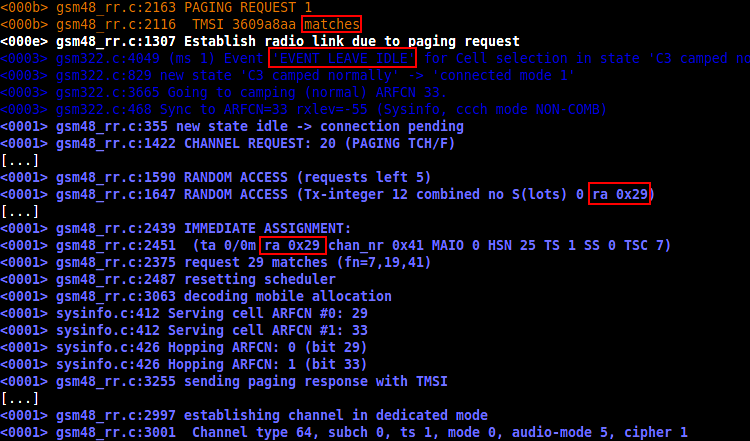
\includegraphics[width=\textwidth]{mobile_rach}
        \caption{Immediate assignment procedure logs in \prog{mobile}}
        \label{fig:mobile_rach}
      \end{figure}

    When in dedicated mode, the network can initiate the dedicated
    channel assignment procedure by sending an Assignment Command
    message to the \gls{ms} on the main signaling link. Upon reception,
    the \gls{ms} commands to switch to the assigned channels described
    in the message. If the main signaling link is successfully
    established, the \gls{ms} returns an Assignment Complete message to
    the network on the main \gls{dcch}. If the establishment fails, it
    sends an Assignment failure instead. A successful procedure in the
    \prog{mobile} application is shown on \fref{fig:mobile_asscmd}.

      \begin{figure}
        \centering
        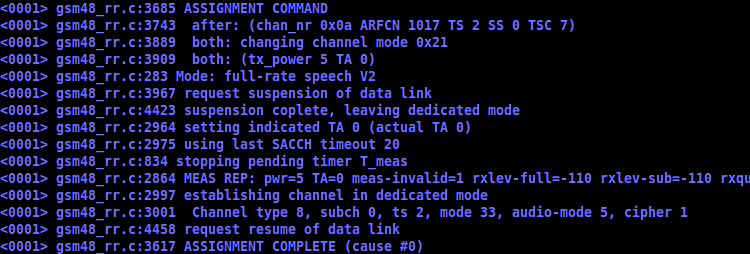
\includegraphics[width=\textwidth]{mobile_asscmd}
        \caption{Dedicated channel assignment procedure logs in \prog{mobile}}
        \label{fig:mobile_asscmd}
      \end{figure}

    In dedicated mode, the network can also initiate a ciphering mode
    setting procedure by sending a Ciphering Mode Command message. This
    contains information about the encryption algorithm to use, if any.
    The \gls{ms} answers with a Ciphering Mode complete message when the
    procedure is over. An example in the \prog{mobile} application is
    given in \fref{fig:mobile_mm}. To go back to idle mode, the
    connection release procedure can be triggered by upper layers, which
    deactivates all the dedicated channel in use. This can be used after
    a call, or when a dedicated channel assigned for signaling is
    released.
    %}

  \subsection{Mobility Management procedures}

    %3GPP TS 24.008 version 12.9.0 Release 12 {
    The \gls{mm} sublayer is used to support the mobility of the various
    \glspl{ms}. For example, by informing the network of their
    locations, or by providing user identity confidentiality. It also
    provides connection management services to the various entities of
    the \gls{cm} sublayer, as well as registration services to the upper
    layers directly. To perform these services, it relies on the
    \gls{rr} sublayer to establish a connection between the \gls{ms} and
    the network~\cite{3gpp_ts_2015-5}. 
    %}

    %3GPP TS 24.008 version 12.9.0 Release 12 {
    Depending on how they are initiated, three types of \gls{mm}
    procedures can be distinguished: common procedures, specific
    procedures, and connection management procedures. All of these will
    be investigated in turn. This section does not provide an exhaustive
    list of procedures, but focuses on the relevant ones for this
    thesis. All these procedures are implemented in the \prog{mobile}
    application again. The code can be found in the
    \code{src/host/layer23/src/mobile/gsm48\_mm.c} file.

    \subsubsection{Common procedures}
    \label{sec:mm_proc_com}

    The purpose of the \gls{tmsi} reallocation procedure is to prevent a
    user from being identified and located by an attacker. Usually it is
    performed at least at each location area change. The network
    initiates this procedure by sending a \gls{tmsi} Reallocation
    Command message to the \gls{ms} containing a new combination of
    \gls{tmsi} and \gls{lai}.  Upon reception, the \gls{ms} stores them
    in the SIM and sends a \gls{tmsi} Reallocation Complete message to
    the network.

    The purpose of the authentication procedure is twofold: it permits
    the network to check whether the identity provided by the \gls{ms}
    is acceptable or not, and it provides parameters enabling the
    \gls{ms} to calculate a new ciphering key. This procedure is always
    controlled by the network which initiates it by sending an
    Authentication Request message. The \gls{ms} then processes the
    challenge information, computes a new key, and sends back an
    Authentication Response message to the network. If it is not valid,
    the network sends an Authentication Reject message to the \gls{ms}.

      \begin{figure}
        \centering
        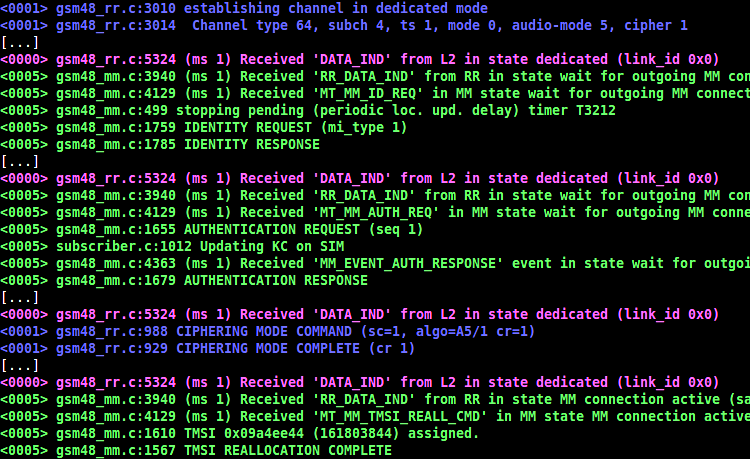
\includegraphics[width=\textwidth]{mobile_mm}
        \caption{Identification, authentication, ciphering mode setting, and TMSI
        reallocation procedures logs in \prog{mobile}}
        \label{fig:mobile_mm}
      \end{figure}

    The identification procedure is used by the network to request an
    \gls{ms} to provide specific identification parameters to the
    network, like its \gls{imsi} or \gls{imei}. The network initiates
    the identification procedure by transferring an Identity Request
    message. Upon reception, the \gls{ms} sends back an Identity
    Response message containing the identification parameters as
    requested by the network. An example of these three procedures in
    the \prog{mobile} application is shown on \fref{fig:mobile_mm}.

    The \gls{imsi} detach procedure may be invoked by an \gls{ms} if the
    phone is turned off or if the \gls{sim} is removed. It consists of
    the \gls{imsi} Detach Indication message sent from the \gls{ms} to
    the network. When receiving this message, the network may set an
    inactive indication for the \gls{imsi}, but this is optional. No
    response is returned to the mobile station. This procedure is shown
    in the \prog{mobile} application on \fref{fig:mobile_detach}.

      \begin{figure}
        \centering
        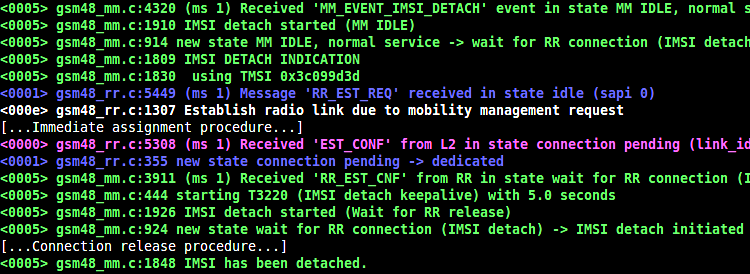
\includegraphics[width=\textwidth]{mobile_detach_s}
        \caption{IMSI detach procedure logs in \prog{mobile}}
        \label{fig:mobile_detach}
      \end{figure}

    \subsubsection{Specific procedures}
    \label{sec:mm_proc_spec}

    The specific procedures are all variations of the location updating
    procedure, which is used for the following purposes: normal location
    updating, periodic updating, or \gls{imsi} attach. All of them
    follow the same pattern and are initiated by the \gls{ms} which
    sends a Location Updating Request message specifying the location
    update variation to the network. The network might then initiate
    various common procedures, for example a \gls{tmsi} reallocation or
    an identification procedure to obtain needed parameters. Depending
    on these parameters, it answers with a Location Updating Accept or
    Reject message.

    The normal location updating procedure is used to update the
    registration of the current location area of an \gls{ms} in the
  network. The \gls{ms} will also start the normal location updating
  procedure if the network indicates that the mobile station is
  unknown in the \gls{vlr} as a response to an \gls{mm} connection
  establishment request. Periodic updating may be used to notify the
  availability of the \gls{ms} to the network at specified intervals.
  The \gls{imsi} attach procedure is the complement of the \gls{imsi}
  detach procedure, and is used to indicate the \gls{imsi} as active
  in the network. An example of an \gls{imsi} attach procedure in
  \prog{mobile} is shown on \fref{fig:mobile_loc_up} and
  \fref{fig:mobile_loc_acc}.

    \begin{figure}
      \centering
      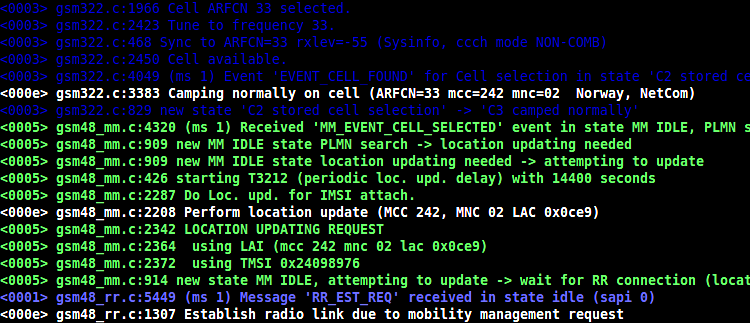
\includegraphics[width=\textwidth]{mobile_loc_up}
      \caption{IMSI attach procedure logs in \prog{mobile}: Location
      Updating Request}
      \label{fig:mobile_loc_up}
    \end{figure}

    \begin{figure}
      \centering
      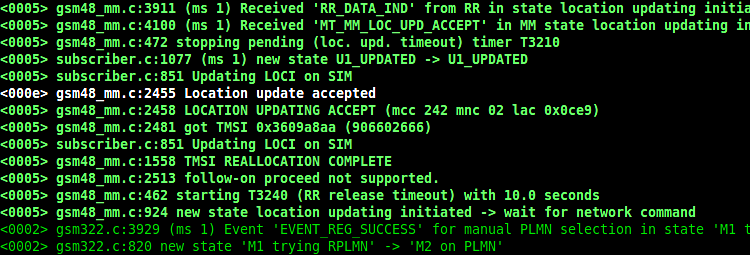
\includegraphics[width=\textwidth]{mobile_loc_acc}
      \caption{IMSI attach procedure logs in \prog{mobile}: Location
      Updating Accept}
      \label{fig:mobile_loc_acc}
    \end{figure}

  \subsubsection{Connection management procedures}

  The \gls{mm} sublayer provides connection management services to the
  various entities of the upper \gls{cm} sublayer upon request from a
  \gls{cm} entity. The connection management procedures are used for
  establishing, re-establishing, maintaining, and releasing an
  \gls{mm} connection.

  In order to establish an \gls{mm} connection, the \gls{mm} sublayer
  sends a \gls{cm} Service Request message to the network. Upon
  reception, the network may start any of the \gls{mm} common
  procedures and \gls{rr} procedures to obtain further information on
  the \gls{ms}. Upon reception of a \gls{cm} Service Accept message,
  the \gls{cm} entity that requested the \gls{mm} connection is
  informed, and the connection is considered to be active. If the
  service request can not be accepted, the network returns a \gls{cm}
  Service Reject message to the \gls{ms}.

  After the \gls{mm} connection has been established, it can be used
  by the \gls{cm} sublayer entity for information transfer. A \gls{cm}
  sublayer entity can then request the transfer of \gls{cm} messages
  which are sent to the \gls{mm} sublayer and transfered to the other
  side of the Um interface. Upon receiving a \gls{cm} message, the
  \gls{cm} sublayer will distribute it to the relevant \gls{cm}
  entity. If the received message is the first for the \gls{mm}
  connection, the \gls{mm} sublayer will in addition indicate to that
  entity that a new connection has been established. An established
  \gls{mm} connection can be released by the local \gls{cm} entity.
  This is done locally in the \gls{mm} sublayer without sending
  messages over the radio interface for this purpose.

  \subsubsection{Location updating example}

  An example of the Location updating procedure is shown on
  \fref{fig:flow_loc_upd}. The \gls{mm} sublayer of the \gls{ms}
  requests an \gls{rr} connection establishment. The \gls{rr} sublayer
  then starts the immediate assignment procedure and sends a Channel
  Request messages on the \gls{rach}. The network answers with an
  Immediate Assignment message.

  Once the dedicated channel is established, the \gls{mm} sublayer
  performs the authentication procedure. Then the ciphering mode
  setting procedure is completed between the \gls{rr} sublayer
  entities. An identification procedure and a \gls{tmsi}
  reallocation procedure could also be scheduled at this point.
  Finally, the network \gls{mm} sublayer sends a Location Updating
  Accept message, and the connection is released.

    \begin{figure}
      \centering
      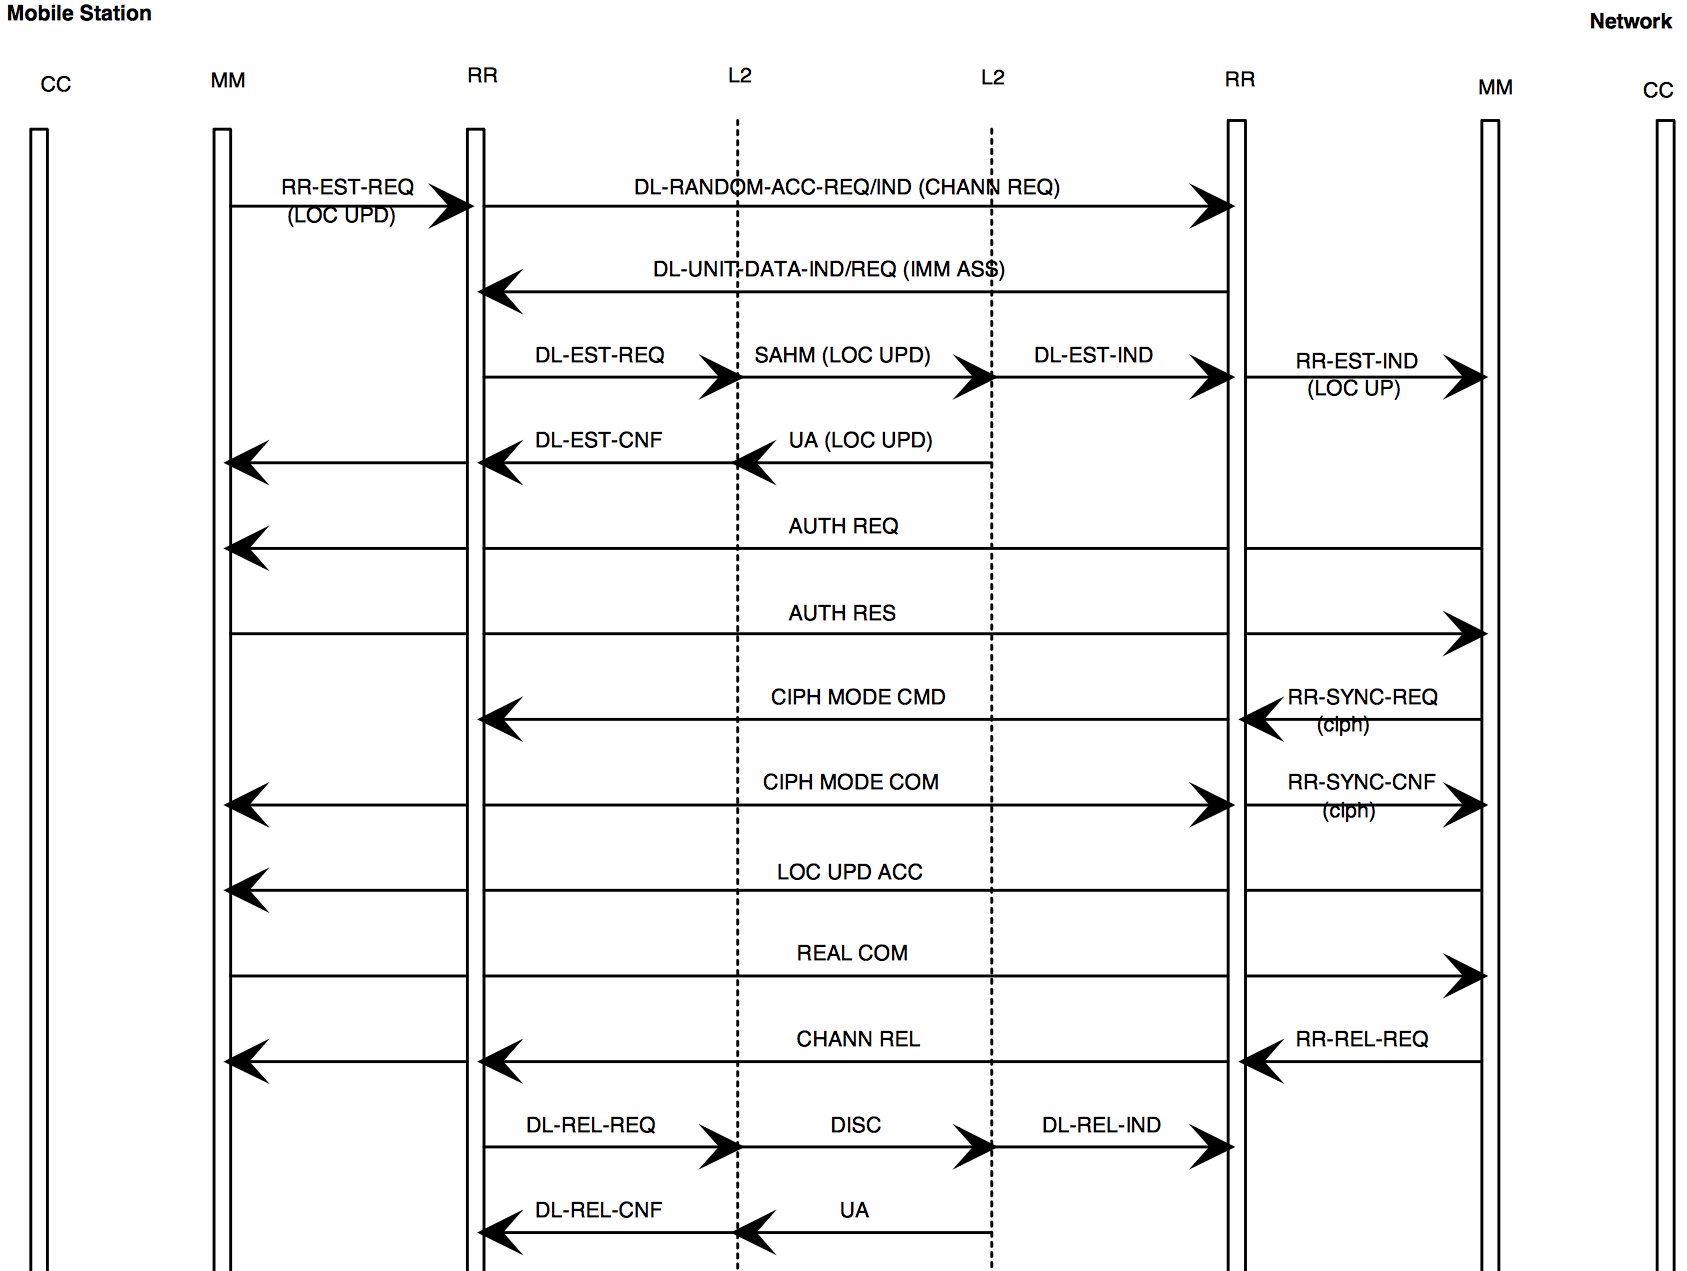
\includegraphics[width=\textwidth]{flow_loc_upd}
      \caption{Location updating procedure flow
      diagram~\cite[p.~117]{3gpp_ts_2014-6}}
      \label{fig:flow_loc_upd}
    \end{figure}

\subsection{Connection Management}

  %3GPP TS 24.008 version 12.9.0 Release 12 {
  The \gls{cm} sublayer relies on the \gls{mm} sublayer to provide
  connection management services. It is subdivided in at least three
  mandatory entities: the \gls{ss} entities, the \gls{sms} entities,
  and the \gls{cc} entities. The last one is used for establishing,
  maintaining, and releasing normal voice calls, whether they are
  \gls{moc} or \gls{mtc}, or \gls{moc} emergency calls. It is
  implemented in the \code{mobile/gsm48\_cc.c} file. The other
  entities are not investigated here~\cite{3gpp_ts_2015-5}.
%}
  \iffalse
  \subsubsection{Short Message Services}

    %3GPP TS 24.011 version 12.0.0 Release 12 {o
  The \gls{sms} entity on the \gls{ms} implements two protocols to
  communicate over the Um interface: the \gls{smcp}, and the
  \gls{smrp}. The first one is used to communicate between two
  \gls{smc} entities, while the second one is used to communicate
  between two \gls{smr} entities. An \gls{smc} entity is part of the
  \gls{cm} sublayer and provides services to the \gls{smr} entity,
  part of the \gls{smr} layer. Finally, the \gls{smr} layer provides
  services to the \gls{smt} layer. 

  When a message transfer is requested by the \gls{smt} layer, the
  \gls{smr} entity sends an RP-Data message to the \gls{smc} entity.
  The \gls{smc} entity will then establish an \gls{mm} connection and,
  when it is ready, send a CP-Data message. If the receiving \gls{smc}
  entity can accept the data, it transmits the message to the
  \gls{smr} layer and answers with a CP-Ack message. Otherwise it
  sends a CP-Error message. The sending \gls{smc} entity will then
  respectively transmit an RP-Ack or RP-Error message to the sending
  \gls{smr} entity.

  These procedures are implemented in the \prog{mobile} application of
  \proj{OsmocomBB} and can be found in
  \code{mobile/gsm411\_sms.c}.
    %}
  \fi

  \subsubsection{Call Control procedures}

%3GPP TS 24.008 version 12.9.0 Release 12 {
  Two \gls{cc} entity procedures are relevant: the call establishment
  procedures, and the call clearing procedures. The call establishment
  procedures consists of several steps and can be of two types: the
  \gls{moc} establishment, or the \gls{mtc} establishment. Both of
  them are reviewed together. An example of the whole procedure is
  described in the next section.

  On the originating \gls{ms}, the \gls{cc} entity initiates
  establishment of a \gls{cc} connection by requesting the \gls{mm}
  sublayer to establish an \gls{mm} connection. Upon establishment of
  this connection, the \gls{cc} entity sends a Setup or Emergency
  Setup message to the network. The setup message will contain all
    the information required by the network to process the call. The
    network answers with a Call Proceeding message to indicate that the
    call is being processed.

    The network will then indicate the arrival of a call to the
    terminating \gls{ms} which will establish a \gls{cc} connection to
    receive the Setup message. Upon reception, it will answer with a
    Call confirm message. It will then start alerting the user and send
    an Alerting message to the network. The network transfers the
    Alerting message to the originating \gls{ms}. If the terminating
    \gls{ms} accepts the call, it sends a Connect message to the
    network. The network will answer with a Connect Acknowledge message,
    connect the traffic channel between the two parties, and send  a
    Connect message to the originating \gls{ms}. The later answers with
    a Connect Acknowledge message and will attach the user connection.

    The clearing procedure is started when either of the two parties
    sends a Disconnect message to the network. Upon reception, the
    network sends a Release message to the other party and starts the
    procedures to release the connections. The \gls{ms} answers with a
    Release Complete message.

    \subsection{Mobile Terminating Call example}

    This section gives an example of a successful \gls{mtc}
    establishment and release. Flow diagrams are available in
    \fref{fig:flow_mtc_setup} and \fref{fig:flow_moc_release}, and logs
    of the \prog{mobile} applications are show in
    \fref{fig:mobile_mtc_setup} and \fref{fig:mobile_mtc_release}. These
    two examples use most of the procedures described in this chapter,
    and will serve as a summary.

    On the flow diagram of \fref{fig:flow_mtc_setup}, the procedure is
    initiated by the \gls{cc} entity of the network, which requests the
    establishment of an \gls{mm} connection. The \gls{mm} sublayer then
    requests an \gls{rr} connection, and the \gls{rr} sublayer starts
    the immediate assignment procedure. It consists of the Paging
    Request, Channel Request, and Immediate Assignment messages. When it
    is over, the \gls{mm} sublayer in the network receives an \gls{rr}
    Establishment Confirmation, while the \gls{mm} sublayer in the
    \gls{ms} receives an \gls{rr} Establishment Indication.

    When the channel is established, the authentication procedure
    between the \gls{mm} sublayers starts. This can be followed by the
    identification procedure, which is not displayed on this diagram.
    Then the \gls{rr} sublayer of the network initiates a ciphering mode
    setting procedure. Again, this could be followed by a \gls{tmsi}
    reallocation procedure which is not shown.
    
    At this point, the \gls{cc} entity on the network side receives an
    \gls{mm} Establishment Confirmation, and sends the Setup message to
    the \gls{cc} entity on the \gls{ms}. This message is also used as an
    \gls{mm} Establishment Indication message. If the establishment
    succeeds, the communication will switch to a traffic channel thanks
    to the dedicated channel assignment procedure. When on the traffic
    channel, the call setup is resumed, and if it succeeds, the voice
    data starts flowing.

    The clearing procedure is displayed on \fref{fig:flow_moc_release}.
    The \gls{cc} entities release the \gls{mm} connection. The \gls{mm}
    sublayer releases the \gls{rr} connection, and finally the data link
    layer releases the data link connection.

      \begin{figure}
        \centering
        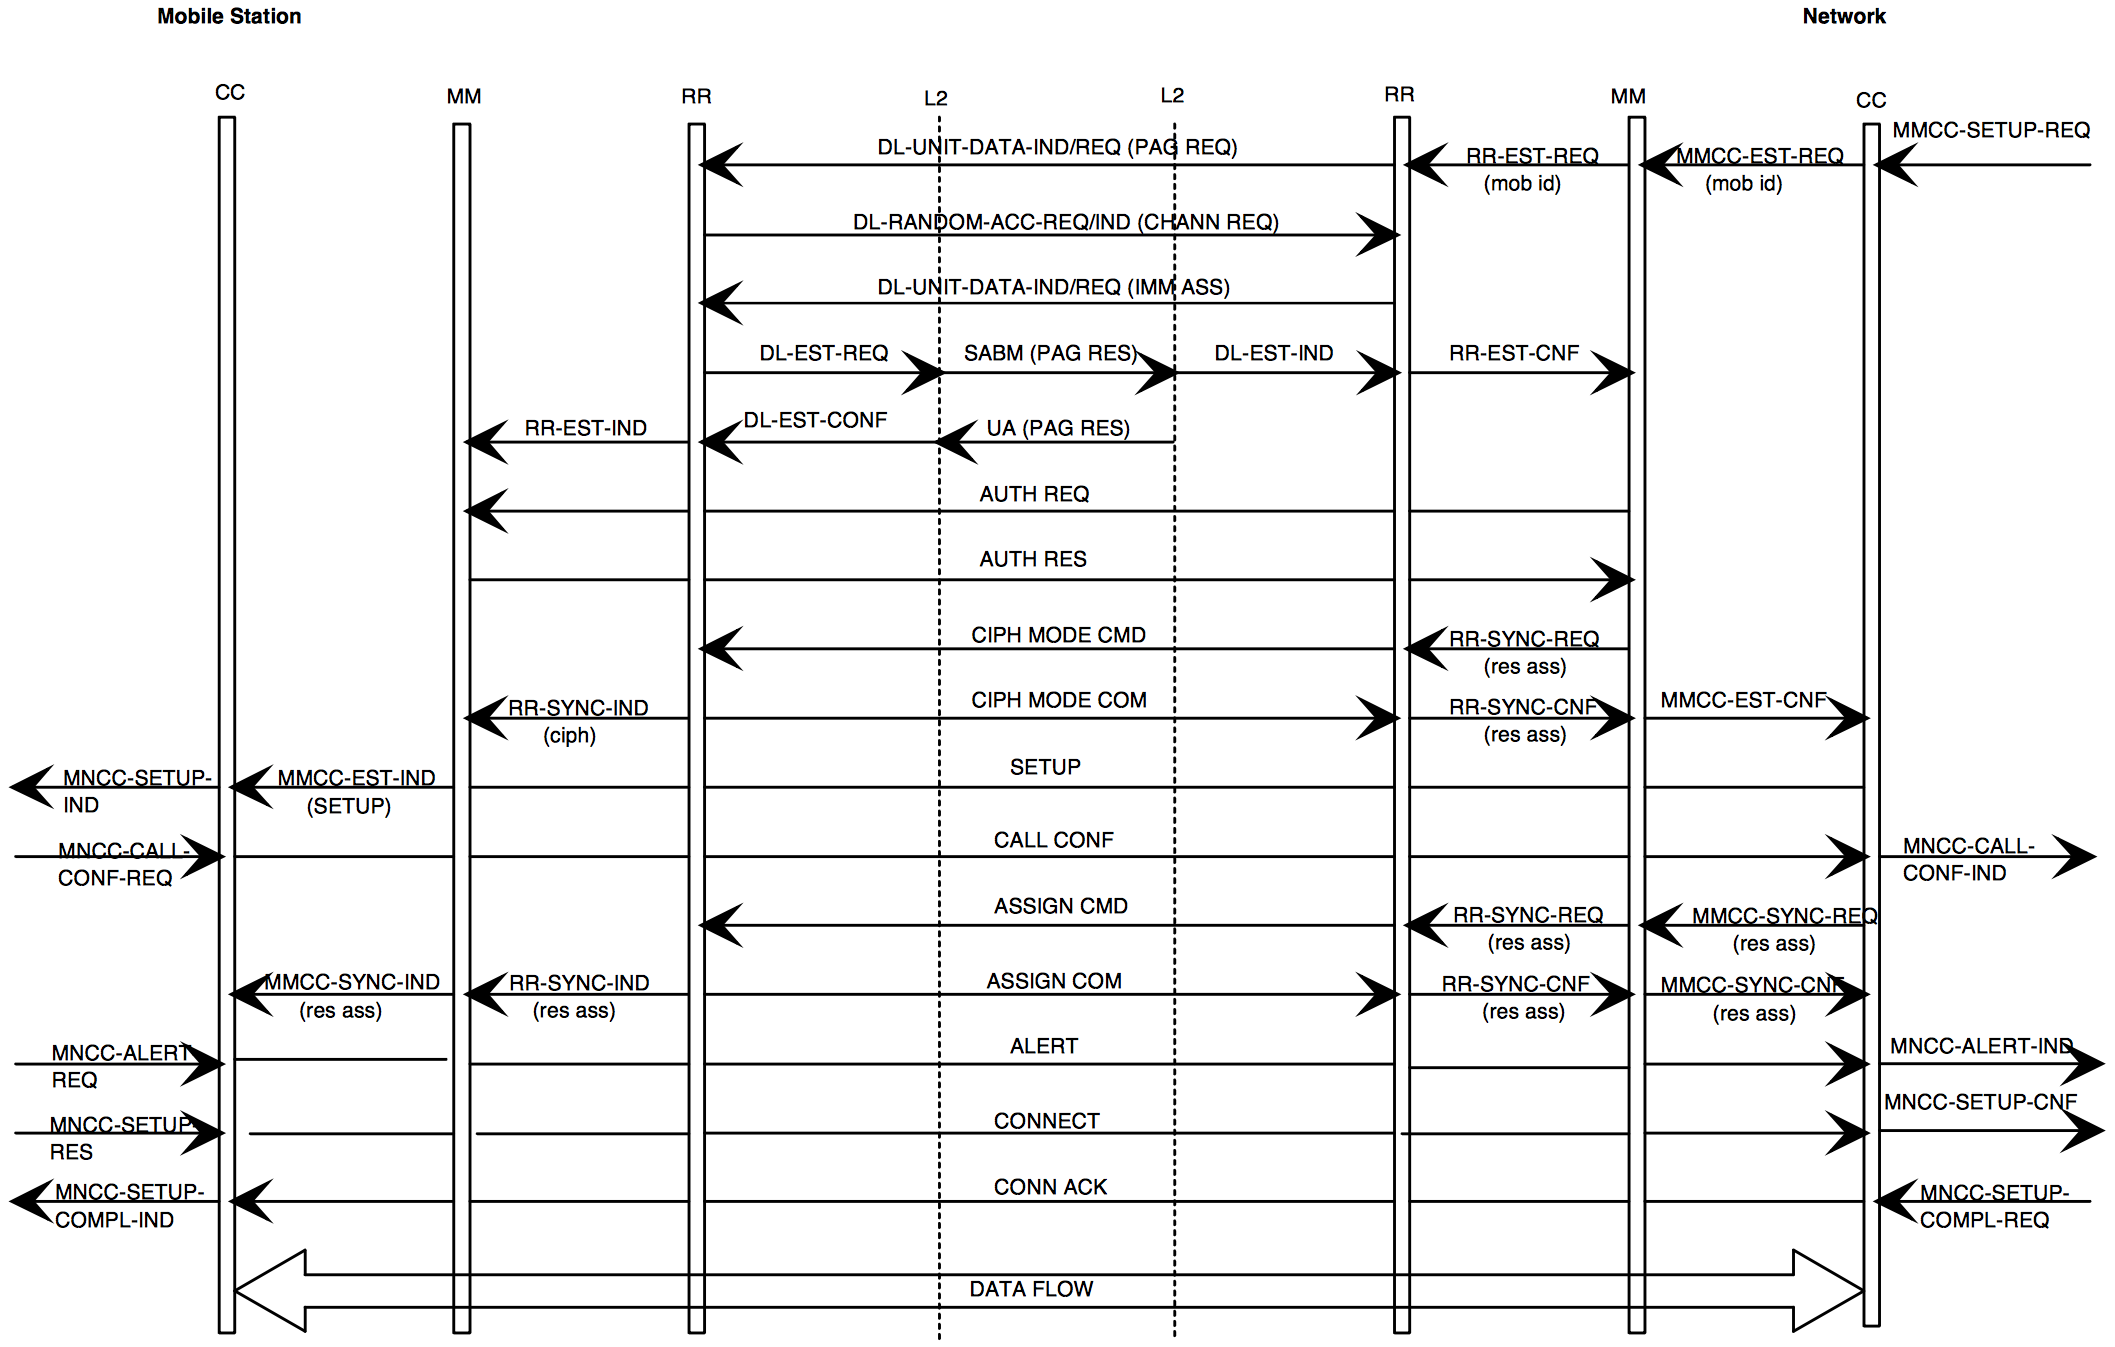
\includegraphics[width=\textwidth]{flow_mtc_setup}
        \caption{Mobile Terminated Call
        setup~\cite[p.~115]{3gpp_ts_2014-6}}
        \label{fig:flow_mtc_setup}
      \end{figure}

      \begin{figure}
        \centering
        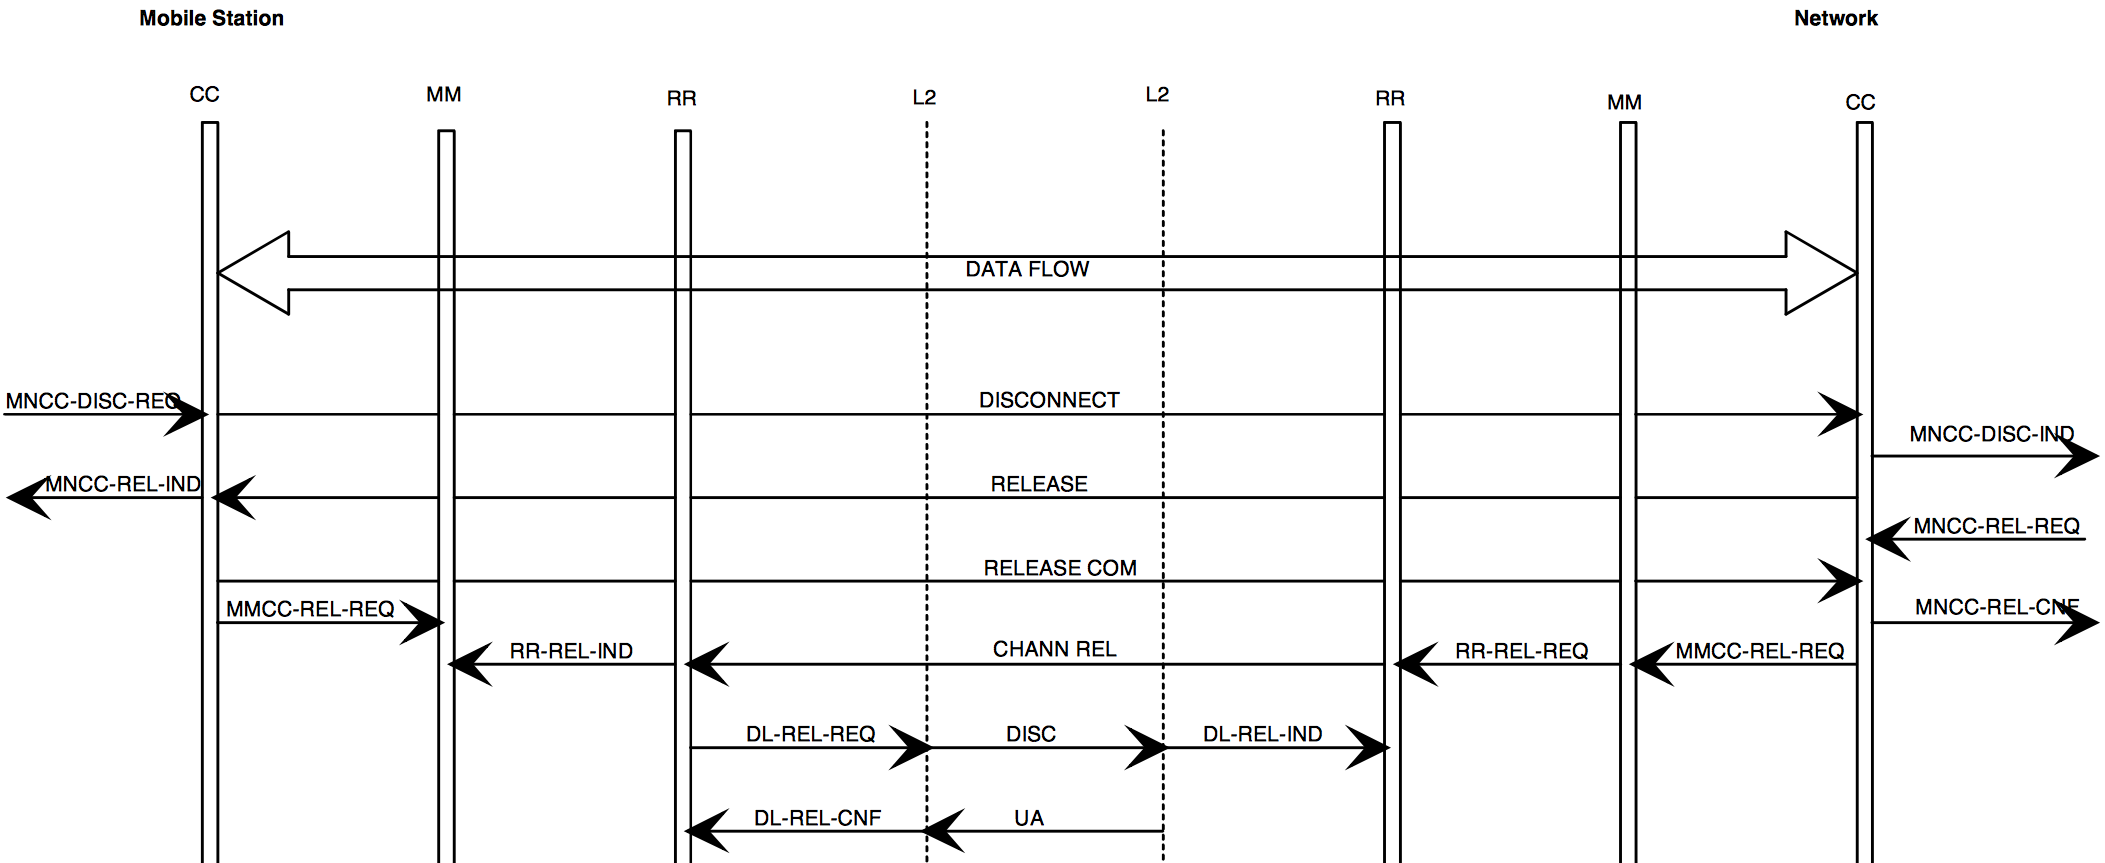
\includegraphics[width=\textwidth]{flow_moc_release}
        \caption{Mobile Originating Call
        release~\cite[p.~116]{3gpp_ts_2014-6}}
        \label{fig:flow_moc_release}
      \end{figure}

      \begin{figure}
        \centering
        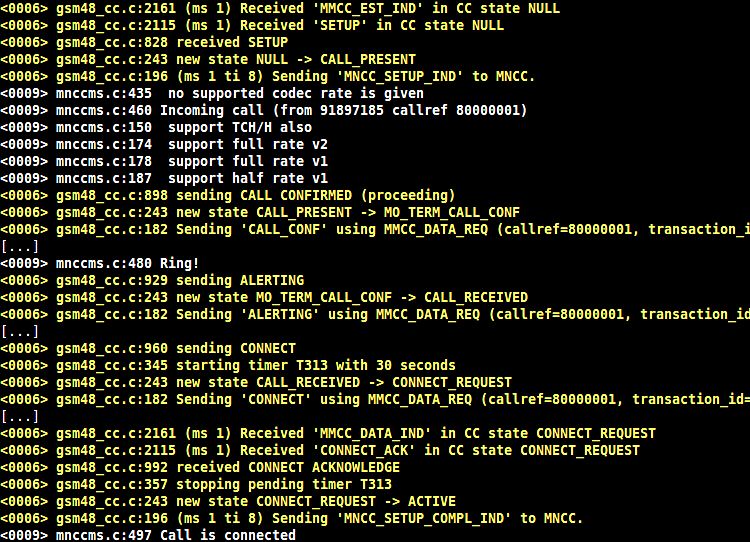
\includegraphics[width=\textwidth]{mobile_mtc_setup}
        \caption{Mobile Terminated Call
          setup in \prog{mobile}~\cite[p.~115]{3gpp_ts_2014-6}}
        \label{fig:mobile_mtc_setup}
      \end{figure}

      \begin{figure}
        \centering
        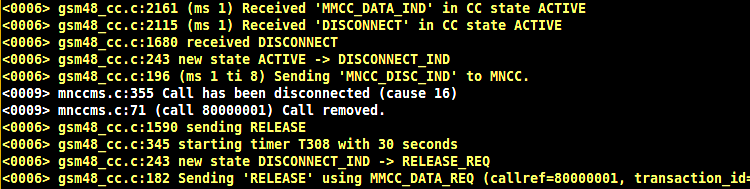
\includegraphics[width=\textwidth]{mobile_mtc_release}
        \caption{Mobile Terminating Call
        release in \prog{mobile}~\cite[p.~116]{3gpp_ts_2014-6}}
        \label{fig:mobile_mtc_release}
      \end{figure}

      \iffalse
  \section{OsmocomBB applications}

    The \prog{mobile} application was used along this chapter to
    demonstrate the various procedures of \gls{gsm}. It is not the only
    application available.


    The point of this chapter is too link the specifications with the
    \proj{OsmocomBB} project. To do so, various applications of the
    project will be introduced. The last one, \prog{mobile}, will be
    used to 



    using osmocombb applications
      ~\cite{osmocombb_applications}
      ~\cite{osmocombb_overview}

    \subsection{Osmocon}

    \iffalse
      \begin{figure}[h]
        \centering
        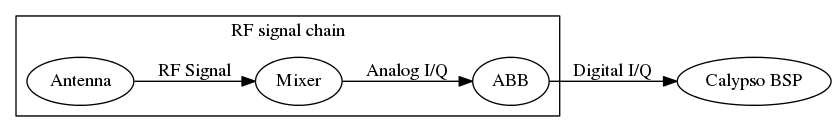
\includegraphics[width=\textwidth]{osmocombb_arch1}
        \caption{~\cite{osmocombb_overview}}
        \label{fig:osmocombb_arch1}
      \end{figure}

      \begin{figure}[h]
        \centering
        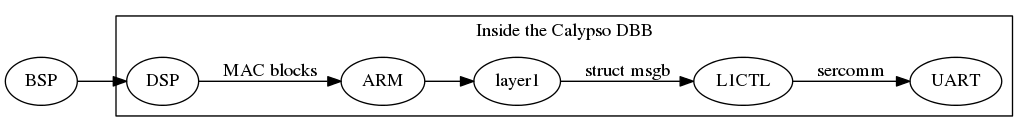
\includegraphics[width=\textwidth]{osmocombb_arch2}
        \caption{~\cite{osmocombb_overview}}
        \label{fig:osmocombb_arch2}
      \end{figure}

      \begin{figure}[h]
        \centering
        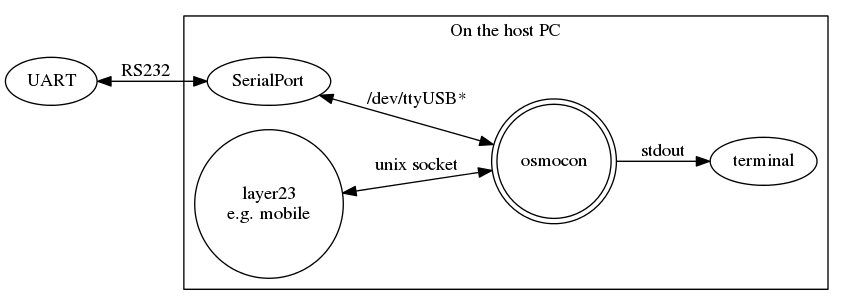
\includegraphics[width=\textwidth]{osmocombb_arch3}
        \caption{~\cite{osmocombb_overview}}
        \label{fig:osmocombb_arch3}
      \end{figure}
      \fi

      \begin{figure}
        \centering
        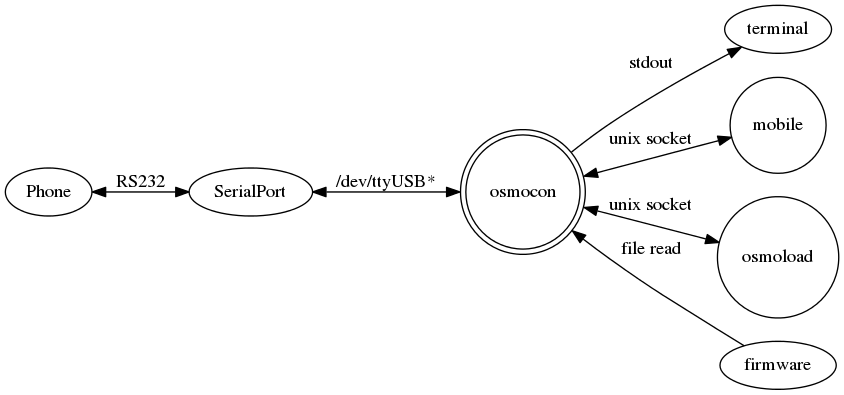
\includegraphics[width=\textwidth]{osmocon}
        \caption{~\cite{osmocombb_osmocon}}
        \label{fig:osmocon}
      \end{figure}

    \subsection{\prog{cell\_log}}

    \iffalse
       The cell_log application scans through valid available carrier
       frequencies, attempts to sync to them and dumps information
       gathered from the BCCH.

       It is usually used to create a list of used ARFCNs and
       information such as their reception levels, MNC, MCC, and System
       Information. 
       \fi

       Scans the bcch.

      \begin{figure}[h]
        \centering
        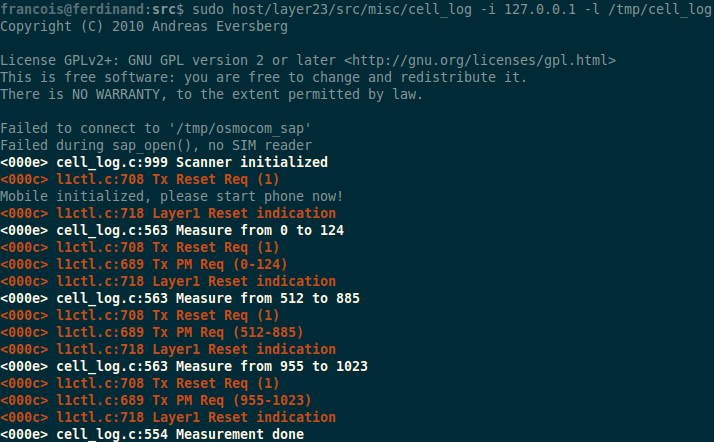
\includegraphics[width=\textwidth]{app_cell_log}
        \caption{The \prog{cell\_log} application first scans through
        all the ARFCNs, and measures their power level.}
        \label{fig:app_cell_log}
      \end{figure}

      \begin{figure}[h]
        \centering
        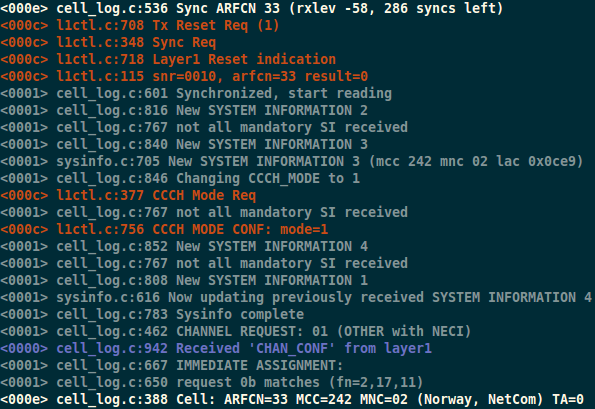
\includegraphics[width=\textwidth]{app_cell_log1}
        \caption{Then, starting with the best received ARFCN, it
          synchronizes with the cell, and gather information from the
          BCCH. Finally, it sends a Channel Request message and listens
          to the Immediate Assignment message to determine the Timing
          Advance parameter.}
        \label{fig:app_cell_log1}
      \end{figure}

      \begin{lstlisting}[language=C, numbers=left,
      basicstyle=\footnotesize, breaklines=true, frame=single]
        [sysinfo]
        arfcn 33
        time 1433681748
        bsic 5,7
        rxlev -56
        si1 55 06 19 00 00 00 00 00 00 00 00 00 00 00 01 10 00 00 00 a5 00 00 2b
        si2 59 06 1a 00 00 00 00 00 00 00 00 00 00 94 04 32 98 18 d0 df a5 00 00
        si3 49 06 1b fa fb 42 f2 20 0c e9 c8 02 28 24 45 40 a5 00 00 80 00 01 1b
        si4 31 06 1c 42 f2 20 0c e9 45 40 a5 00 00 80 00 4b 2b 2b 2b 2b 2b 2b 2b
        ta 0
        \end{lstlisting}
    
    \subsection{\prog{ccch\_scan}}

    \iffalse
    The ccch_scan application can sync to a carrier ARFCN and logs power
    measurement and CCCH information (paging requests and Immediate
    Assignments). 
    \fi

      Scans the ccch.

      \begin{figure}[h]
        \centering
        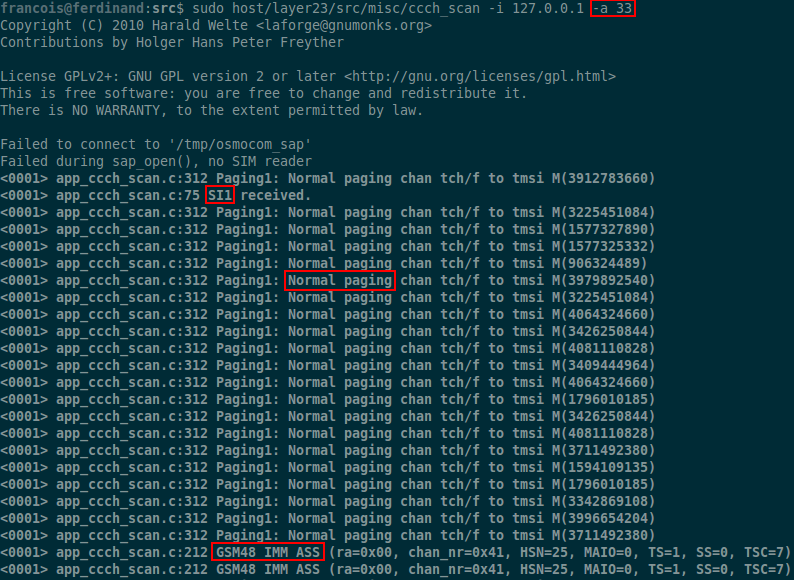
\includegraphics[width=\textwidth]{app_ccch_scan}
        \caption{This application scans the CCCH of a given ARFCN. It
        first reads SI1 and SI3 to get the needed parameters, then it
      listens and displays the Paging Request messages on the PCH, and
    the Immediate Assignment messages on the AGCH.}
        \label{fig:app_ccch_scan}
      \end{figure}

    \subsection{\prog{mobile}}

    \iffalse
     mobile is the most sophisticated OsmocomBB application so far.

     It implements most of the behavior of a regular GSM telephone, but
     is extended in many ways with features interesting to researchers. 
     \fi

     \url{http://bb.osmocom.org/trac/wiki/mobile}


     \iffalse
      The mobile program is one of the various host (PC) based programs
      that you can use together with the layer1.*.bin firmware images
      inside the phone.

      mobile is the most sophisticated OsmocomBB application so far. It
      implements most of the behavior of a regular GSM telephone, but is
      extended in many ways with features interesting to researchers.

      Using mobile, you can e.g.

          perform cell (re)selection according to TS 03.22
              MM procedures like location updating, authentication,
              encryption
                  Establish MT and MO voice calls
                      Send and receive SMS
                          Perform supplementary services like USSD or
                          call forwarding
                              hook it up to a PBX 

                              In the spirit of all Osmocom projects, the
                              user interface of mobile is based on text
                              commands issued on the command line. 
    \fi


    \iffalse
      \begin{figure}[h]
        \centering
        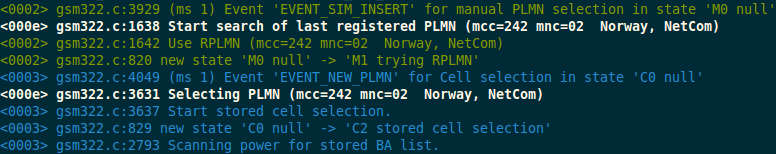
\includegraphics[width=\textwidth]{mobile_sim_insert}
        \caption{.}
        \label{fig:mobile_sim_insert}
      \end{figure}
      \begin{figure}[h]
        \centering
        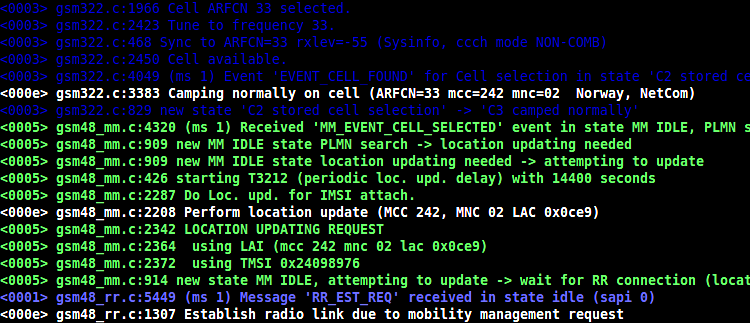
\includegraphics[width=\textwidth]{mobile_loc_up}
        \caption{.}
        \label{fig:mobile_loc_up}
      \end{figure}
      \begin{figure}[h]
        \centering
        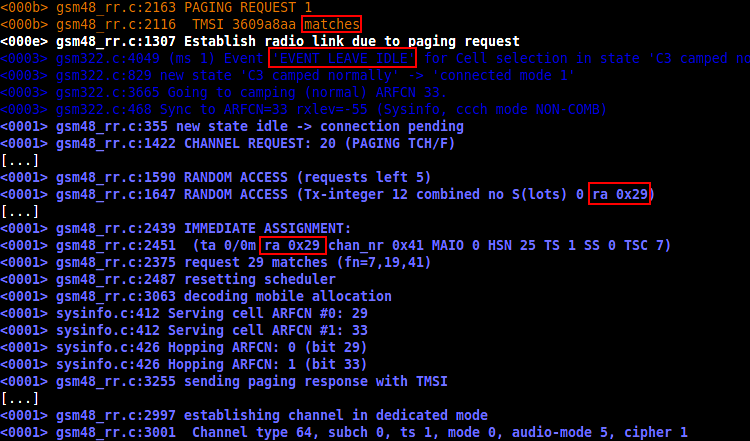
\includegraphics[width=\textwidth]{mobile_rach}
        \caption{.}
        \label{fig:mobile_rach}
      \end{figure}
      \begin{figure}[h]
        \centering
        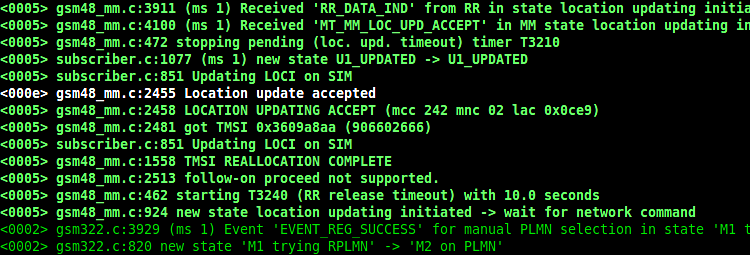
\includegraphics[width=\textwidth]{mobile_loc_acc}
        \caption{.}
        \label{fig:mobile_loc_acc}
      \end{figure}
      \begin{figure}[h]
        \centering
        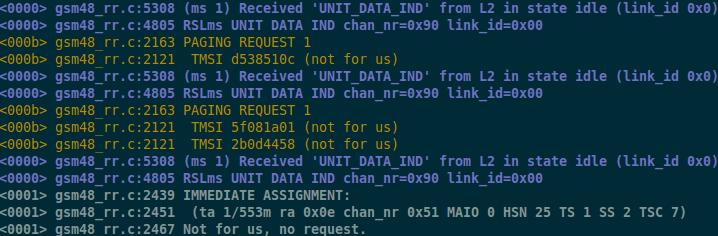
\includegraphics[width=\textwidth]{mobile_idle}
        \caption{.}
        \label{fig:mobile_idle}
      \end{figure}
      \begin{figure}[h]
        \centering
        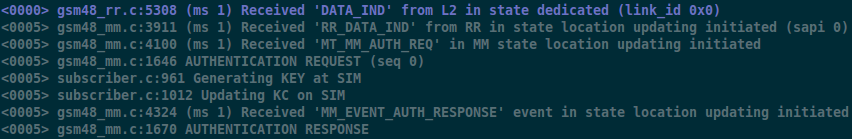
\includegraphics[width=\textwidth]{mobile_auth}
        \caption{.}
        \label{fig:mobile_auth}
      \end{figure}
      \begin{figure}[h]
        \centering
        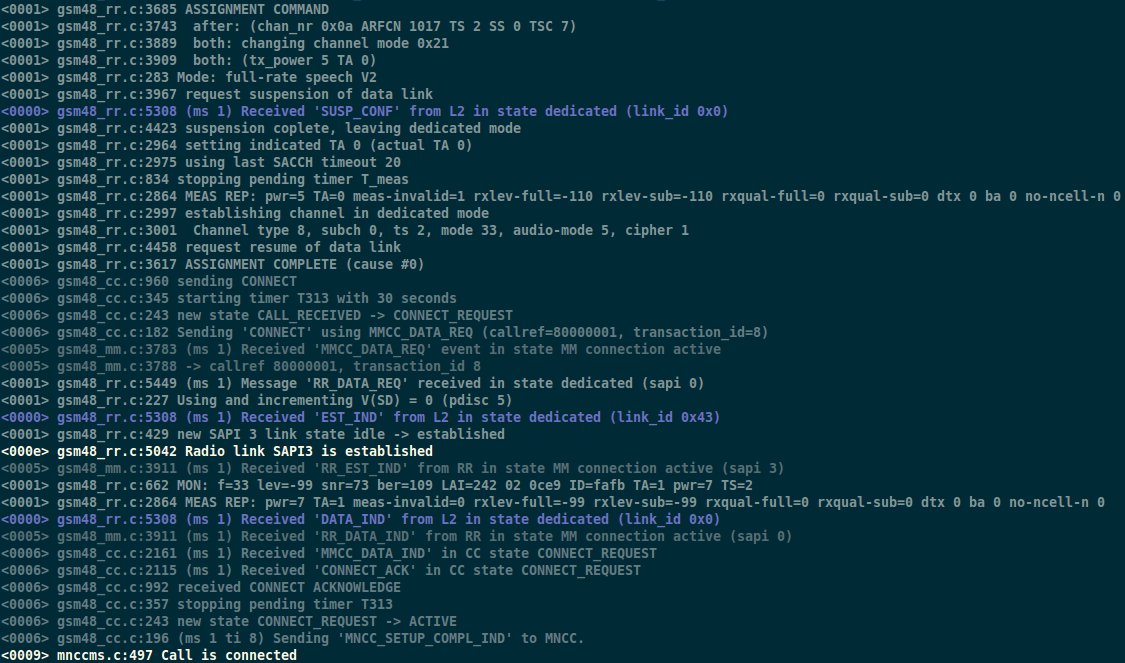
\includegraphics[width=\textwidth]{mobile_connect}
        \caption{.}
        \label{fig:mobile_connect}
      \end{figure}
      \begin{figure}[h]
        \centering
        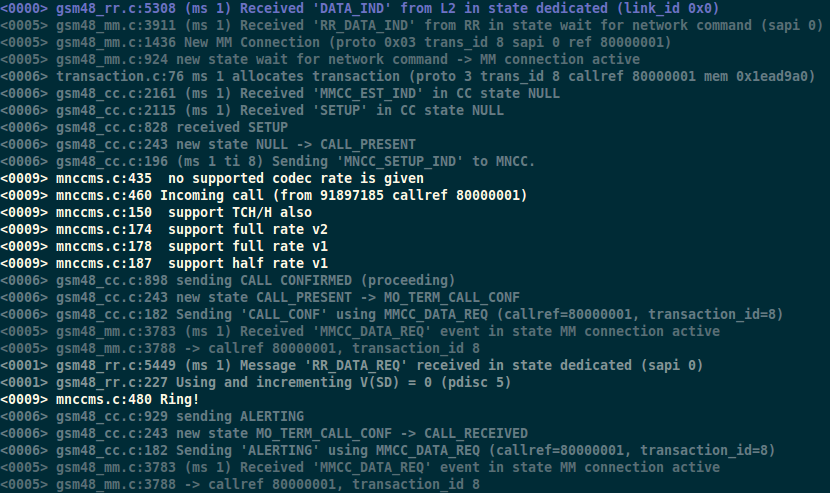
\includegraphics[width=\textwidth]{mobile_alerting}
        \caption{.}
        \label{fig:mobile_alerting}
      \end{figure}
      \begin{figure}[h]
        \centering
        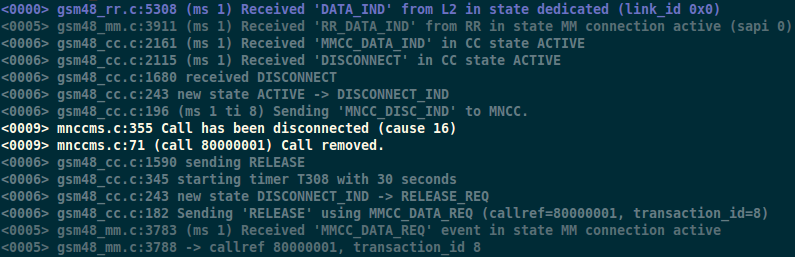
\includegraphics[width=\textwidth]{mobile_release}
        \caption{.}
        \label{fig:mobile_alerting}
      \end{figure}
      \begin{figure}[h]
        \centering
        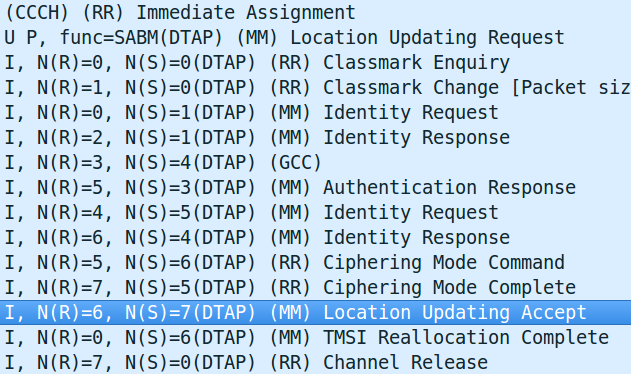
\includegraphics[width=\textwidth]{mobile_ws_lu}
        \caption{.}
        \label{fig:mobile_ws_lu}
      \end{figure}
      \begin{figure}[h]
        \centering
        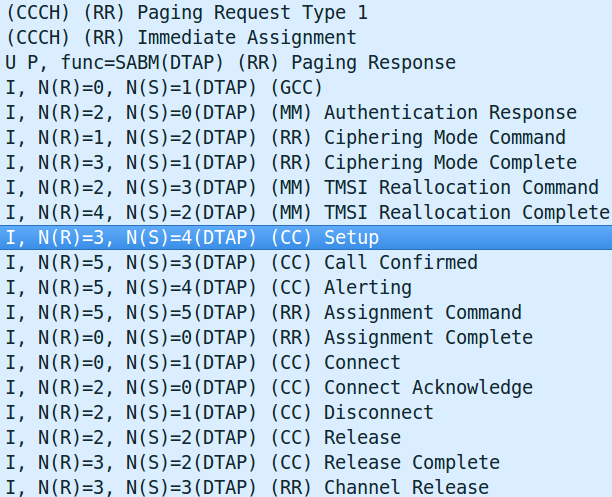
\includegraphics[width=\textwidth]{mobile_ws_mtc}
        \caption{.}
        \label{fig:mobile_ws_mtc}
      \end{figure}
      \begin{figure}[h]
        \centering
        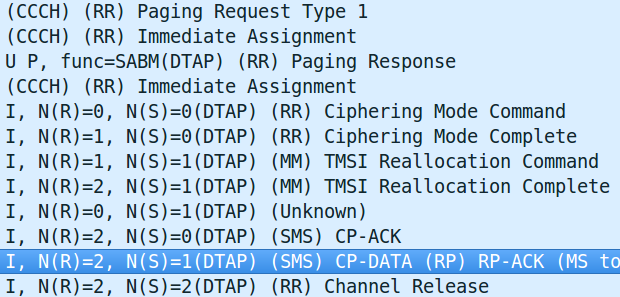
\includegraphics[width=\textwidth]{mobile_ws_mtsms}
        \caption{.}
        \label{fig:mobile_ws_mtsms}
      \end{figure}
      \fi
      \fi

\chapter{Eavesdropping attacks} \label{chap:eavesdropping_attacks}

\iffalse
    The whole attack could not be
    carried out, 
    
    Insist on the implementation and
    detailed explanation, this is the product. The whole attack could
    not be carried out. I think no publication shows how to do it and
    the only one was Munaut at 27C3. Really not trivial. try to explain
    the method and to give it a nice name. How i tried to solve the pb
    and implement the code
    \fi

    This chapter will focus on two eavesdropping attacks using
    \proj{OsmocomBB}: one on \gls{gsm}, the other on \gls{gprs}. The
    first section of the chapter explains the role of \proj{OsmocomBB}
    in the attack. It describes the way it was used to take a different
    approach to the problem by creating a passive listener exploiting
    dedicated hardware. The next sections are dedicated to the four
    steps of the attack.

    The first one consists of finding the location of the target, and
    the second one consists of finding its \gls{tmsi}. The \gls{tmsi}
    and location of the subscriber are linked, since the purpose of the
    \gls{tmsi} is to provide confidentiality to the subscriber by
    preventing attackers to track its location. Therefore, these two
    steps are also linked. The third step consists in finding the
    session key of the target. Encryption is applied by the network to
    provide data confidentiality, and to prevent eavesdropping. It is
    thus necessary to find this key to be able to eavesdrop on the
    communication. Finally, the last step is to capture this
    communication on the Um interface and to decode
    it~\cite{3gpp_ts_2006}.

    Various applications and commands of the \proj{OsmocomBB} project
    are detailed in this chapter. \Sref{app:tuto} of the appendices is
    available to describe their installation and usage. Some
    modifications were also done to these applications for the purpose
    of this thesis and some of them are described in context in this
    chapter. Explanations on how to apply these modifications are also
    available in the appendices.

  \section{\proj{OsmocomBB} as a passive listener}
  \label{sec:passive_listener}

    Before the availability of the \proj{OsmocomBB} project, the usual
    method to capture \gls{gsm} signals was to use an \gls{usrp} device
    combined with tools from the \proj{Airprobe} project. These tools,
    introduced in~\Sref{sec:airprobe}, were not optimal for several
    reasons. Firstly, this system could not effectively follow frequency
    hopping. Secondly, the received signal was a bit unreliable.
    Finally, capturing uplink traffic was complicated. The
    \proj{OsmocomBB} project is based on an actual mobile phone, which
    means that it uses hardware dedicated to \gls{gsm}. A mobile phone
    is designed to switch between frequencies very quickly, and to
    demodulate and decode uplink and downlink \gls{gsm} signals.
    Therefore, \proj{OsmocomBB} does not suffer from the same problems,
    and was a good candidate as a basis for an eavesdropping attack.

    Eavesdropping requires the attacker to break the encryption applied
    on the communication. A tool exists to find A5/1 session keys,
    \proj{Kraken}, but it expects some keystream generated using this
    key. Finding keystream requires to XOR a bitstream of plaintext and
    ciphertext. However, \proj{OsmocomBB} relies on the phone modem to
    produce layer 2 packets, as explained in~\Sref{sec:modem}. Since the
    encryption process is applied at a very low level, this does not
    give access to the encrypted keystream.

    For that purpose, \name{Sylvain Munaut} demonstrated at DeepSec 2010
    how it was possible to create a passive listener from one of the
    phones supported by \proj{OsmocomBB}, and to extract the bits off
    the air just after the demodulation and without further
    processing~\cite{munaut_cheap_2010}. This makes it possible to
    capture keystream to find the associated session key. It is also
    possible to use code from \proj{Airprobe} programs to convert these
    bits to upper layer packets. As a bonus, this listener supports
    uplink capture, can follow frequency hopping, has a very good
    demodulation, and is very inexpensive. 

    \begin{figure}
      \centering
      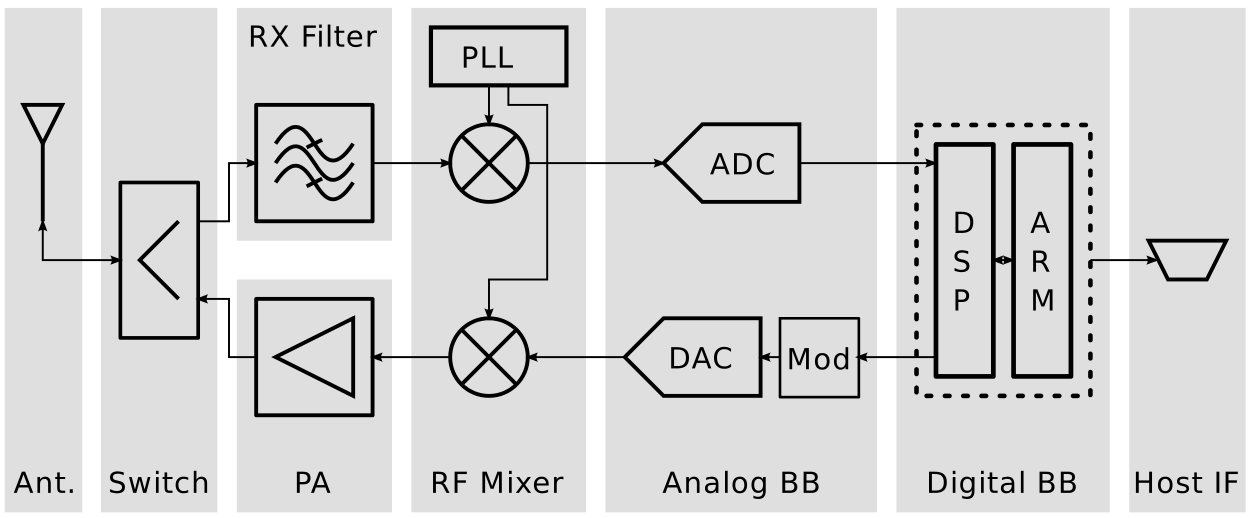
\includegraphics[width=\textwidth]{typical_calypso_platform}
      \caption{Block diagram of a typical Calypso
              platform~\cite{munaut_further_2012}}
      \label{fig:typical_calypso_platform}
    \end{figure}

    A simplified diagram of the receive and transmit path of a typical
    Calypso platform is shown on \fref{fig:typical_calypso_platform}.
    More information on that topic is available in~\Sref{sec:modem}.
    What interests us here is the upper part of the figure: the
    receive path. It is composed of several components and each of
    them could be an obstacle to the implementation of the listener.

    \begin{itemize}[topsep=-1em,parsep=0em,itemsep=0.5em]

      \item The antenna is completely common. In case of uplink capture,
        it could be replaced by another antenna, but it is not really
        necessary.

      \item The antenna switch splits the signal between the receive
        path and the transmit path, and does not cause any problem.

      \item The reception filter reduces the noise by attenuating every
        signal which is not at the received downlink frequency by around
        \SI{35}{\deci\bel}. This means that it strongly attenuates the
        received uplink signal which is already weak. It can be replaced
        to increase the uplink reception range from less than
        \SI{20}{\meter} to around \SI{150}{\meter}, but the operation is
        delicate due to the components size.

      \item The \gls{rf} mixer tunes the phone to any frequency in the
        four downlink bands. The uplink bands are out of the
        specifications, but after removing the dedicated verification
        functions, the \gls{pll} can be configured to support them as
        well. Of course, the results are a bit poorer, but not
        significantly. The mixer also needs to be configured to deal with at
        least two consecutive bursts instead of one, to receive the
        uplink as well. This is possible since multislot is a feature of
        \gls{gprs} which is supported by the Calypso
        platform.

      \item The analog baseband is simply an \gls{adc} in this case, and
        the demodulation is done in the \gls{dsp}. It receives I/Q
        symbols and converts them to digital samples coded as soft
        bits.

      \item The first part of the digital baseband is the \gls{dsp}.
        When used in normal operation, it processes the digital signal
        to reconstruct a layer 2 packet. The traffic bursts are
        decompressed inside the \gls{dsp} and sent directly to the audio
        codec. The \gls{dsp} firmware is stored in a mask \gls{rom}, but
        part of the \gls{ram} can be used to patch it. This is done by
        overwriting entries in a function table to provide new functions
        stored in \gls{ram}. The new functions modify the \gls{dsp}
        behavior to send the demodulated bits to the second part of the
        digital baseband without further processing.

      \item The second part of the digital baseband is an ARM processor
        which hosts the \proj{OsmocomBB} firmware. This makes it easier
        to apply the four necessary modifications. The first is to use
        the \gls{dsp} bootloader to patch the \gls{rom} and provide the
        functions for the sniffing task in \gls{ram}. The second is to
        add this task to the \gls{dsp} driver. The third is to use it in
        the \gls{dsp} to get the raw demodulated bits. The last is to
        replace data transmission by the reception of the uplink
        frequency using the same task.

      \item The last component is the serial interface used to
        communicate with the host computer. After the modifications in
        the receiving path, it has to transmit 4 bursts of 116 soft bits
        every \SI{4.615}{\milli\second}, which requires non standard
        baud rates.\fxnote{Why four and not two? Because it might be
        useful in the future?}

    \end{itemize}

    After all these modifications, the listener is able to receive the
    demodulated bursts in up to four time slots per frame, for the
    downlink or the uplink. These are saved in a file that can be
    decoded using parts of the programs available in \proj{Airprobe}. To
    summarize, the impact of this \proj{OsmocomBB} based passive
    listener comes from its good uplink support, its hardware dedicated
    to frequency hopping and \gls{gsm} signal processing, and its wide
    availability. The modifications applied to \proj{OsmocomBB} to
    create a passive listener are available in the
    \code{sylvain/burst\_ind} branch of the project git repository. The
    filter replacement, as well as the choice of a suitable USB to RS232
    converter, is described on the project website.

    An example of the output of a modified version of the
    \prog{ccch\_scan} application is shown on \fref{fig:log_bi}. This
    application is intended as a small demonstration of what is possible
    using this passive listener. The \gls{ms} will follow any Immediate
    Assignment message to the dedicated channel, and will save all the
    relevant bursts to a file. On the figure, four bursts received in
    four consecutive frames are highlighted twice: once for the
    downlink, and once for the uplink. The layer 2 message is contained
    into these four bursts due to the interleaving process. Once the
    four bursts are received, they are deinterleaved and decoded to a
    layer 2 message, which is sent to \proj{Wireshark} via
    \prog{gsmtap}.

    \begin{figure}[h]
      \centering
      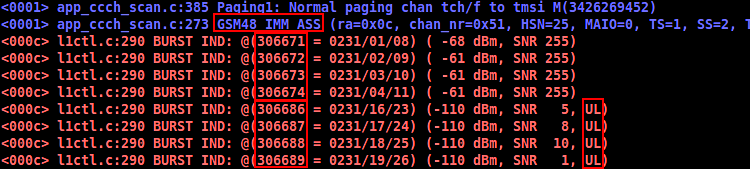
\includegraphics[width=\textwidth]{log_bi}
      \caption{Output of the \prog{ccch\_scan} application in the
        \code{burst\_ind} branch.\fxnote{cfr gsm time!}}
      \label{fig:log_bi}
    \end{figure}

    \iffalse On Mon, Aug 29, 2011 at 01:55:59AM +0200, Lukas Kuzmiak
    wrote: > If I'm not mistaken pl2303 based cables have/had problems
    handling baudrates > above 115200, there was a recent update into
    the kernel tree, but I've never > tested it.

the problem is not "[standard] baud rates above 115200" but it is
"non-standard baud-rates at all".  Normal USARTs have baud-rate
generators that can only generate baud-rates "input_clock / divider"
where divider is either an integer, or even more: limited to a power of
2

The calypso cannot do any standard baud-rates above 115200.  That's why
you need a USART with more flexible baud rate generator.  The most
commonly known one to do this is the FTDI series of USB-serial
converters. 
    \fi

  \section{Recovering the location}

    After describing how to create a passive listener, the details of
    the attack itself will be investigated. The attacker needs to be in
    the same cell as the targeted phone since everything happens on the
    Um interface. If the location of the target is not known, it is
    possible to exploit the \gls{ss7} to find relevant information. The
    \gls{ss7} contains various protocols that are used in the telephony
    world. One of them, the \gls{map}, was designed to provide signaling
    services between various elements of the mobile networks and is
    introduced in~\Sref{sec:ss7}. Two services described there can be
    exploited to get location information for a given subscriber if an
    access to the network is available.

    \subsection{Accessing the SS7}

      According to \name{James Moran}, the security director for the
      \gls{gsma}: \textquote{SS7 is inherently insecure, and it was
      never designed to be secure}~\cite{timberg_for_2014}. This makes
      it difficult for the operators to prevent abuses. Nevertheless,
      good filtering policies could reduce the attack surface but, at
      the end of 2014, \name{Karsten Nohl} said that many operators do
      not implement them. Moreover, some \gls{ss7} services are needed
      for normal network operation, and thus are almost impossible to
      filter. This allows anyone with a roaming agreement and an access
      to the \gls{ss7} to request this
      information~\cite{nohl_mobile_2014}.

      According to \name{Tobias Engel}, \textquote{getting access to the
      SS7 is easier than ever}, and since legitimate commercial services
      need it, it \textquote{can be bought from telecom operators or
      roaming hubs for a few hundred euros a month}. He also said that
      \textquote{some network operators leave their equipment unsecured
      on the Internet}. Another access vector could be femtocells.
      Indeed, since they are part of the core networks but placed in
      subscribers homes, it could be possible to hack them to get an
      access~\cite{engel_ss7:_2014}.

    \subsection{HLR query}
    \label{sssection:hlr_query}

      An \gls{hlr} query is a name commonly used for a
      MAP-SEND-ROUTING-INFO-FOR-SM service request, which is described
      in more details in~\Sref{sec:sriforsm}. A way of exploiting this
      service was presented by \name{Tobias Engel} at the
      25C3~\cite{engel_locating_2008}.

      It is easy to see on \fref{fig:map_srifs_hl} that during a
      legitimate \gls{sms} delivery procedure, the \gls{gmsc} requests
      information from the \gls{hlr}, and then sends the \gls{sms}
      message on its own. This can be exploited because the fourth step on
      the diagram is actually optional. Having access to the \gls{ss7},
      it is therefore possible to request information from the \gls{hlr}
      and never send any \gls{sms} message. The information returned is,
      based on a subscriber phone number, the \gls{imsi} of the
      subscriber as well as the number of the \gls{msc} serving it.

      \begin{figure}[h]
        \centering
        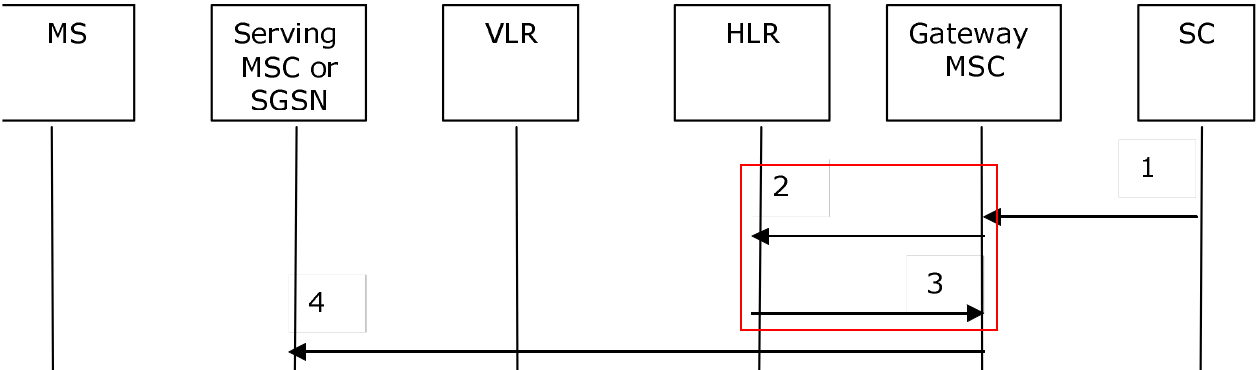
\includegraphics[width=\textwidth]{map_srifs_hl}
        \caption{Exploiting the MT-SMS
      procedure~\cite[p.~792]{3gpp_ts_2015-2}.}
        \label{fig:map_srifs_hl}
      \end{figure}

      %http://www.nkom.no/npt/numsys/E.164.pdf
      The number of the \gls{msc} gives information on the current
      location of the mobile phone, since it starts with a country code.
      It also gives information on the operator to which the phone is
      currently connected to thanks to its identification code. The
      result of an \gls{hlr} query displaying the number of the
      \gls{msc} is shown on \fref{fig:location}. On this example, the
      country code, 47, belongs to Norway, and the identification code,
      92, belongs to \comp{Netcom}~\cite{nkom}.

      \begin{figure}
        \centering
        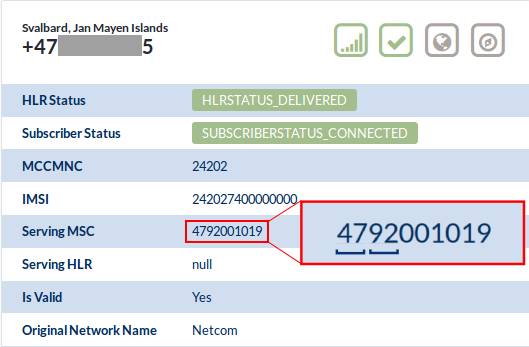
\includegraphics[width=\textwidth]{location}
        \caption{MSC number returned from an HLR query.}
        \label{fig:location}
      \end{figure}
      
      These \gls{hlr} queries allow to build databases providing a
      mapping between an \gls{msc} number and a location by querying
      phones in known locations. An example presented by
      \name{Tobias Engel} for Germany is shown on
      \fref{fig:location_te}. The area that an \gls{msc} covers might be
      a part of a city, a whole city or even bigger. Indeed, an
      \gls{msc} usually handles a certain amount of traffic and
      therefore the area it covers depends on the population density.
      Thus, determining the \gls{msc} where the phone is located is only
      a first step to uncover the location of the targeted phone.

      \begin{figure}
        \centering
        \includegraphics[width=\textwidth]{location_te}
        \caption{Mapping between MSC numbers and
        location~\cite{engel_locating_2008}}
        \label{fig:location_te}
      \end{figure}

      To find the cell of interest, two methods can be used. Either
      wardriving, which is explained in \Sref{sec:recovering_tmsi},
      or a \gls{psi} service request. While it is easy to find companies
      providing cheap and easy to use \gls{hlr} queries online,
      \gls{psi} requests are more difficult to access.

    \subsection{MAP PSI service}

      PSI service is a short name for the MAP-PROVIDE-SUBSCRIBER-Info
      service described in~\Sref{sec:psi}. At the 31C3, \name{Karsten
      Nohl} showed how it was possible to exploit it to recover a more
      precise location than with an \gls{hlr} query
      alone~\cite{nohl_mobile_2014}. Indeed, an \gls{hlr} query gives
      the \gls{imsi} of the subscriber based on its phone number, while
      a PSI service request gives the \gls{cgi} related to this
      \gls{imsi}. The \gls{cgi} is composed of the \gls{mcc}, the
      \gls{mnc}, the \gls{lac}, and the Cell ID, as explained in
      \Sref{sec:cgi}. This allows one to easily find the location of the
      target by querying one of the Cell ID database available online.

    \section{Recovering the TMSI}
    \label{sec:recovering_tmsi}
      
      The previous step gave out the location of the target and the cell
      it is camping on. It is now necessary to find out the identity of
      the target on this cell to be able to follow its calls on the
      dedicated channel. The \gls{tmsi} can not be queried over the
      \gls{ss7} \gls{map} protocol, so another method is used to recover
      it.
      
      It works by contacting the targeted phone according to a given
      pattern and by listening to the beacon channel looking for a
      \gls{tmsi} getting paged according to the same pattern. This makes
      the assumption that the \gls{tmsi} will stay the same between the
      beginning and the end of the process. Listening to the beacon
      channel can be done with a mobile phone using the
      \code{ccch\_scan} application available in \proj{OsmocomBB}. An
      example of its output is shown on \fref{fig:log_tmsi}.

      \begin{figure}[h]
        \centering
        \includegraphics[width=\textwidth]{log_tmsi}
      \caption{Output of the \prog{ccch\_scan} application.}
        \label{fig:log_tmsi}
      \end{figure}

      This method can also be used to refine the location granularity
      after a simple \gls{hlr} query. Every paging request is sent on
      the whole location area, so by looking for the pagings in each of
      the location area served by the serving \gls{msc}, it is possible
      to determine if the targeted phone is there or not. The same
      method can be applied to find the \gls{cgi}. The attacker can go
      from one cell to another and look for the paging responses sent by
      the targeted \gls{tmsi}, to make sure to be in the right cell.
      This is called wardriving.

      To make sure that the user of the targeted phone does not notice
      this step, it is possible to send so called silent \gls{sms}
      messages, which are not displayed on the targeted
      phone~\cite[p.~53]{3gpp_ts_2001}. If they are blocked by the
      operator, it is also possible to send broken \gls{sms} messages
      that the mobile discards but this is dependent of the baseband
      implementation~\cite{golde_sms-o-death:_2011}. A last method
      consists of initiating a phone call, and hanging up after the
      paging is done, but before the user is
      alerted~\cite{kune_location_2012}.

      An implementation of the silent \gls{sms} feature is proposed with
      this thesis. Each \gls{sms} message contains a
      TP-Protocol-Identifier field, and setting its value to \code{0x40}
      tells the receiving \gls{ms} to discard its contents. This means
      that the targeted \gls{ms} is paged, but that nothing shows up on
      the targeted user's screen. This is called a type 0 \gls{sms}.
      Another field that can be modified is the TP-Data-Coding-Scheme
      field, which indicates whether or not an \gls{sms} message is
      compressed. It consists of two bytes, and if the first byte is set
      to \code{0xC0}, the \gls{ms} may discard the contents of the
      message~\cite[p.~6]{etsi_gsm_1999}. The patch can be found in the
      appendices \Sref{app:patches} and provides the \prog{silent}
      command in the \prog{mobile} application of \proj{OsmocomBB}, as
      displayed in \fref{fig:mobile_silent}. An implementation of the
      correlation feature could not be developed since Norwegian
      networks reallocate the \gls{tmsi} too often, as discussed
      in~\Sref{sec:tmsi_realloc}.

      \begin{figure}
        \centering
        \includegraphics[width=\textwidth]{mobile_silent}
        \caption{Set TP-PID and TP-DCS fields using the patched
        \prog{mobile} application}
        \label{fig:mobile_silent}
      \end{figure}
      
    \section{Finding the session key}
    \label{sec:finding_kc}

      Once the location and identity of the target are found, it is
      necessary to uncover the session key before being able to capture
      a call. This is needed to decrypt the traffic of course, but also
      to find out the frequencies on which the traffic is sent. Indeed,
      the traffic channel is assigned by an Assignment Command sent on
      the dedicated channel after enabling the encryption, as explained
      in \Sref{sec:rr_proc}. The session key needs to be found before
      the Assignment Command to be able to capture the beginning of the
      call as well. To do so, it is necessary to capture data on the Um
      interface, including the communication and the keystream, and to
      decode it.

      \subsection{Capturing keystream and using \proj{Kraken}}
      \label{sec:keystream_and_kraken}

      The first way of solving this problem makes two assumptions.
      Firstly, the encryption algorithm has to be A5/1 or A5/2, because
      they are broken. Secondly, there should not be any key
      renegotiation between the discovery of the key and the targeted
      call. Some networks assign a session key to be used several times,
      but other renegotiate a new key more often. If the key is
      renegotiated after every \gls{sms} message, this method is
      useless.

      If these assumptions are met, the first step is to page the target
      using one of the method discussed in the previous section, silent
      \gls{sms} messages for example. Since they are sent encrypted on
      the dedicated channel, it is possible to follow them and capture
      some keystream using the passive listener described
      in~\Sref{sec:passive_listener}. Indeed, there is a lot of known
      plaintext in \gls{gsm}. For example, the System Information 5 or 6
      can be found encrypted and unencrypted, as shown on
      \fref{fig:si5_keystream_ws}~\cite{nohl_gsm:_2009}.

        \begin{figure}
          \centering
          \includegraphics[width=\textwidth]{si5_keystream_ws}
          \caption{SI5 sent before and after the Ciphering Mode Command}
          \label{fig:si5_keystream_ws}
        \end{figure}

      The keystream associated with the session key can be recovered
      with a XOR operation on the plaintext and the ciphertext. That
      keystream can then be used to find the session key using
      \proj{Kraken} along with the Berlin table set described in
      \Sref{sec:berlin}, and this session key can serve to follow the
      next phone call, as long as the key did not change.

      Finding keystream can be done with a program proposed with this
      thesis. The patch is available in \Sref{app:keystream} of the
      appendices, and modifies a version of the \prog{ccch\_scan}
      application found in the \code{sylvain/burst\_ind} branch. This
      modified application will follow a given \gls{tmsi} on the
      dedicated channel, and store the plaintext of a System Information
      5 message sent before the Ciphering Mode Command. When the
      encryption is started, it will then try to guess which encrypted
      message is a System Information 5 message based on a sequence
      provided by the user. Finally, it outputs potential keystream by
      applying a XOR operation on the stored plaintext and the
      ciphertext. Its usage is described in the appendices, and an
      example of its output is shown in \fref{fig:keystream}.

        \begin{figure}[h]
          \centering
          \includegraphics[width=\textwidth]{keystream}
          \caption{Output of the modified \prog{ccch\_scan} application
          in the \code{burst\_ind} branch displaying potential
        keystream}
          \label{fig:keystream}
        \end{figure}

      \subsection{MAP Send Identification service}

        A second way of finding the session key exists, which gets rid of
        the previously mentioned assumptions, as long as an access to
        the \gls{ss7} \gls{map} protocol is possible. Firstly, this
        method can provide session keys regardless of the encryption
        algorithm used, even A5/3. Secondly, there is no risk of
        triggering a session key renegotiation simply by using it. This
        technique exploits the MAP\_SEND\_IDENTIFICATION service described
        in~\Sref{sec:si}.

        The request associated with this service can be used to recover
        the session key associated with a \gls{tmsi}, as well as up to
        five authentication sets. The authentication sets, or
        authentication triplets, contain the random challenge, the
        signed response, and the session key for the following
        sessions~\cite[p.~100]{3gpp_ts_2015-1}. Exploitation of this
        service request make the encryption on the Um interface
        irrelevant.

    \section{GSM eavesdropping}

      After describing various ways of recovering the location,
      \gls{tmsi}, and session key of the target, this section will focus
      on the actual call capture and explain how to use the passive
      listener described in \Sref{sec:passive_listener} to create a
      sniffer.

      A sniffer needs to be able to record mobile-terminating services
      as well as mobile-originating ones. When the targeted phone
      initiates a call, there is no paging on the beacon channel since
      the phone sends a request directly. This makes it impossible for
      the sniffer to follow the target on the dedicated channel by
      listening to the paging messages only. This problem is solved by
      following every Immediate Assignment message seen on the beacon
      channel to the dedicated channel. If this Immediate Assignment
      was not addressed to the targeted phone, messages after the
      Ciphering Mode Command could not be decrypted with the session key
      found earlier. If these messages can be decrypted, then the
      Assignment Command is followed to the traffic channel and the call
      recorded.

      On a busy cell, it is common for Immediate Assignment messages to
      be sent very close to each other. The interval can be smaller
      than the time needed for the listener to realize that the
      Immediate Assignment message was not relevant and to synchronize
      on the beacon channel again. Therefore, several listeners are
      needed to build a sniffer capable of processing all the
      assignments messages. To do so, one listener can stick to the
      beacon channel and coordinate the others by assigning them to a
      dedicated channel in turn. The more listeners are available, the
      more Immediate Assignment messages can be followed in parallel.

      When the raw demodulated traffic bursts are saved in a file, a
      program based on \proj{Airprobe} can decode them to audio. This
      means that, under certain conditions, it is possible to eavesdrop
      on the downlink and the uplink of a hopping \gls{gsm} phone calls
      for less than \SI{1500}{kr} or \SI{200}{\euro}.

    \section{GPRS eavesdropping}

      At the Chaos Computer Camp in 2011, \name{Luca Melette} and
      \name{Karsten Nohl} showed how it was possible to use the same
      passive listener as a basis to listen to \gls{gprs} signals as
      well~\cite{melette_gprs_2011}. It seems to be the only public
      attack of this kind, but it is more of a demonstration of what is
      possible and not as complete as what can be done for \gls{gsm}.
      Thus, several steps are missing. For example, the recovery of the
      temporary identity or the session key was not
      shown~\cite{srlabs_gprs_????}.

      Because it is complicated to find all the \gls{gprs} packets, this
      demonstration only works on a single \gls{arfcn} and captures all
      the time slots from the uplink or downlink frames on one channel.
      It uses two listeners to do so, since each of them is able to
      listen to four time slots per frame.

      To decode the captured demodulated raw bits, a new program was
      created: \prog{gprsdecode}. It multiplexes the data from the
      various time slots, then decodes it to the \gls{llc} layer and
      sends it to \proj{Wireshark}, where IP packets can be read. Since
      the \gls{gea} encryption used in \gls{gprs} is not broken yet,
      this only works for unencrypted traffic. Surprisingly, some
      networks did not encrypt traffic at the time of the
      presentation.\fxnote{what about psi requests to get the key?}

  \iffalse

  encryption ss7 : MAP_SEND_AUTHENTICATION_INFO service

  http://baseband-devel.722152.n3.nabble.com/GPRS-Vs-EDGE-Trying-to-decode-my-own-sessions-td3288960.html

  http://baseband-devel.722152.n3.nabble.com/uplink-sniffing-td3531044.html

  http://baseband-devel.722152.n3.nabble.com/GPRS-decode-tutorial-td3437051.html

  http://baseband-devel.722152.n3.nabble.com/Sniffing-GPRS-td3712433.html

  http://baseband-devel.722152.n3.nabble.com/Sniffing-GPRS-td3712433.html

  http://baseband-devel.722152.n3.nabble.com/Working-of-ccch-scan-and-capturing-the-SDCCH-td4025206.html#a4025213

  \fi

\chapter{Denial-of-Service attacks} \label{chap:dos_attacks}

\iffalse
IN DOS, SHOW THE STATE DIAGRAMS FOR THE THINGS I MODIFIED

Cfr protocol implementation chapter for references. It is in rr/mm/cm.


for imsi detach, check att flag. detach is required for both network,
yet it doesn't work on one of them. Try with tmsi?


!!!!!!!!!!!!!!!!TALK ABOUT HOW IT INFLUENCES GPRS AS WELL!!!!!!!!!!!!!!!!!!

    Insist on the implementation and explanation, this
    is the product. Afak, no other publication explaining all the
    available attacks. insist of implementation with mobile, this is new
    and innovative to exploit normal stuff. try to explain teh method
    and give it a nice name. how i tried to solve the pb and implement
    eth code.

\fi

    \proj{OsmocomBB} makes it easy for anyone to send arbitrary messages
    to the network, and this offers various possibilities for \gls{dos}
    attacks. They are four main attacks allowing a \gls{dos} on the GSM
    network and an implementation is proposed for the first three.

    The implementations proposed here are based on the \prog{mobile}
    application of \proj{OsmocomBB} which aims to implement all the
    functions of a normal mobile phone and is introduced
    in~\Cref{chap:protocol_stack_implementation}. It is probably not the
    best choice for attacks relying on sending a high rate of messages
    to the network if the goal is purely efficiency, but these
    implementations are interesting here because they demonstrate that a
    \gls{dos} attack can be performed with some simple modifications of
    normal phone procedures and functions. \fref{fig:mobile_dos} shows
    the \gls{dos} commands added to the \prog{mobile} interface. All
    these commands provide a description and an interactive help in the
    program, and \Sref{app:tuto} of the appendices describe their
    installation and usage.

      \begin{figure}[h]
        \centering
        \includegraphics[width=\textwidth]{mobile_dos}
        \caption{\gls{dos} commands available in the interface of the patched \prog{mobile}
        application.}
        \label{fig:mobile_dos}
      \end{figure}

    The first section is dedicated to the RACHell attack, the second one
    to the \gls{imsi} attach attack, the third one to the \gls{imsi}
    detach attack, and the last one to attacks exploiting paging race
    conditions. Each section proposes a theoretical explanation of the
    related attack followed by an explanation of a proposed
    implementation, and a demonstration of the command usage.

    \section{RACHell}

      \subsection{Theory}

      Even if the theory had been known before, this attack was first
      demonstrated by \name{Dieter Spaar} at DeepSec in 2009 using a
      TSM30 mobile phone, the ancestor of
      \proj{OsmocomBB}~\cite{spaar_practical_2009}. It takes place very
      early in the communication process between the \gls{ms} and the
      network, since it exploits the Channel Request messages that the
      \gls{ms} sends on the \gls{rach}. This means that the phone did
      not send any identification information to the network yet, and
      that the authentication did not take place, which makes this
      attack hard to prevent.

      The channel request process, called the immediate assignment
      procedure, is summarized here but explained in more details
      in~\Sref{sec:rr_proc}. The \gls{ms} sends a Channel Request
      message on the \gls{rach} to the network. Upon reception, the
      network establishes a channel and sends an Immediate Assignment
      message to the \gls{ms}. This message contains the necessary
      information about the newly activated dedicated channel. Two
      things are interesting here. Firstly, the authentication is only
      done on this dedicated channel, after the channel establishment.
      Secondly, the network starts a timer when it receives a channel
      request, and if nothing happens on the channel, it is released
      when that timer elapses.

      The attack is simple since it floods the network with Channel
      Request messages. This has several consequences. Firstly,
      collisions on the channel are possible since the \gls{rach} uses a
      slotted ALOHA approach. Thus, it might prevent legitimate requests
      to even access the network in that cell by effectively jamming the
      channel. Secondly, each cell only has a given number of channels
      to allocate. If it receives more channel requests than that during
      the time needed for the release timer to elapse, this attack will
      exhaust them all. This makes it very difficult for a legitimate
      user to request a channel on that cell, but does not influence
      already existing connections.
      
      \subsection{Implementation}
      \label{sec:rachell_impl}

      The implementation of the RACHell attack proposed for this thesis
      is based on the \prog{mobile} application of \proj{OsmocomBB}. The
      normal behavior of this application is explained
      in~\Sref{sec:rr_proc}. When trying to establish a channel, this
      application will send a given amount of Channel Request messages.
      It stops either when an Immediate Assignment message matching this
      request is received, or when the maximum amount of requests
      allowed by the network is reached.       

      Therefore, two modifications are applied to the \prog{mobile}
      application. The first one consists of significantly increasing
      the maximum amount of requests that are sent before aborting the
      establishment attempt. The second one makes sure that the function
      matching the Immediate Assignment reference never succeeds. These
      modifications force the \gls{ms} to send a continuous flow of
      Channel Request messages to the network. A patch adding the
      \prog{dos rach} command to the \prog{mobile} application is
      available in \Sref{app:patches} of the appendices.

      This attack will target the network on which the \gls{ms} is
      currently camping. Usually, when an \gls{ms} running the
      \prog{mobile} application decides to camp on a network, it will
      start a location update procedure. If this procedure fails, the
      \gls{ms} will camp on the most suitable cell, which might not be
      part of the targeted network. Therefore, the \prog{dos camp}
      command was developed to make the phone believe that the location
      update procedure was already done, and is thus not necessary
      anymore. This makes the phone camp on the targeted network. A
      patch adding this command is available in \Sref{app:patches} of
      the appendices as well.

      To apply a \gls{dos}, it might be good to allow the cell
      reselection process to happen. For example, if the attacker
      follows the victim, the attacker's \gls{ms} will probably
      automatically select the same cell as the victim's \gls{ms} and
      thus deny service to the appropriate one. When the goal is to deny
      service to a given \gls{arfcn}, it is possible to use the
      \prog{stick} command available in the normal \prog{mobile}
      application.

      Others have implemented this attacks, for example \name{the grugq}
      at Black Hat 2010~\cite{the_grugq_base_2010}. Even if the request
      flood is supposed to impact a cell only, he reported taking down a
      \gls{bsc}. An implementation using OsmocomBB as well as some
      measurements were also proposed by Maxim
      Suraev~\cite{suraev_denial--service_2011}.

      \iffalse
need to show example of use and output
maybe in appendices
\fi

      \subsection{Demonstration}
      \label{sec:rachell_demo}
      
      Several figures displaying the various steps of the attacks and
      their output are available. The use of the \prog{dos camp}
      command, as well as the available arguments, is shown on
      \fref{fig:mobile_dos_camp}. \fref{fig:log_dos_camp0} shows how the
      \gls{ms} firsts camps on any cell when no \gls{sim} is inserted.
      \fref{fig:log_dos_camp} shows how the \prog{dos camp} command
      exploits the software \gls{sim} feature to force the \gls{ms} to
      select the requested \gls{plmn}, \comp{Telenor} in this case. A
      location update procedure would be rejected by the network, since
      the \gls{sim} is not valid. Therefore, the \prog{dos camp} command
      tricks the \gls{ms} into considering that the location update is
      not required, as shown on \fref{fig:log_dos_camp2}.

      \begin{figure}
        \centering
        \includegraphics[width=\textwidth]{mobile_dos_camp}
        \caption{Using the \prog{dos camp} command: making the MS camp on
        \comp{Telenor}.}
        \label{fig:mobile_dos_camp}
      \end{figure}

      \begin{figure}
        \centering
        \includegraphics[width=\textwidth]{log_dos_camp0}
        \caption{Using the \prog{dos camp} command: MS camps on any cell
        if no SIM.}
        \label{fig:log_dos_camp0}
      \end{figure}
     
      \begin{figure}
        \centering
        \includegraphics[width=\textwidth]{log_dos_camp}
        \caption{Using the \prog{dos camp} command: using the soft SIM
        functionality to force the MS to select the requested PLMN.}
        \label{fig:log_dos_camp}
      \end{figure}

      \begin{figure}
        \centering
        \includegraphics[width=\textwidth]{log_dos_camp2}
        \caption{Using the \prog{dos camp} command: tricking the MS into
        considering that the location update is not required.}
        \label{fig:log_dos_camp2}
      \end{figure}

      \fref{fig:mobile_dos_rach} shows the use of the \prog{dos camp}
      command in the interface of the \prog{mobile} application to camp
      on the \comp{Netcom} network, and the use of the \prog{dos rach}
      command to send three Channel Request messages to this network.
      Three messages do not constitute a \gls{dos}, but the point is
      not to damage the networks. The logs of the mobile application
      show the effect of the command. \fref{fig:log_dos_rach} shows how
      the \gls{rr} sublayer leaves the idle mode and tries to establish
      a channel. \fref{fig:log_dos_rach2} shows a Channel Request
      message sent on the \gls{rach} with a \gls{rai} of \code{0x00}.
      Finally, \fref{fig:log_dos_rach3} shows Immediate Assignment
      messages sent by the network and containing the same \gls{rai},
      and shows how the \gls{ms} discards them.

      \begin{figure}
        \centering
        \includegraphics[width=\textwidth]{mobile_dos_rach}
        \caption{Using the \prog{dos rach} command: sending three Channel
        Request messages to \comp{Netcom}}
        \label{fig:mobile_dos_rach}
      \end{figure}

      \begin{figure}
        \centering
        \includegraphics[width=\textwidth]{log_dos_rach}
        \caption{Using the \prog{dos rach} command: the MS tries to
        establish a radio link.}
        \label{fig:log_dos_rach}
      \end{figure}

      \begin{figure}
        \centering
        \includegraphics[width=\textwidth]{log_dos_rach2}
        \caption{Using the \prog{dos rach} command: the MS sends 3
          Random Access messages. This one has a RA of \code{0x00}.}
        \label{fig:log_dos_rach2}
      \end{figure}

      \begin{figure}
        \centering
        \includegraphics[width=\textwidth]{log_dos_rach3}
        \caption{Using the \prog{dos rach} command: the MS sees
        Immediate Assignment messages with an RA of \code{0x00}, but
      discards them.}
        \label{fig:log_dos_rach3}
      \end{figure}

      \iffalse
      \begin{figure}
        \centering
        \includegraphics[width=\textwidth]{log_dos_rach4}
        \caption{The MS sees Immediate Assignment messages with an RA
        of \code{0x00}, but discards them. Same in Wireshark.}
        \label{fig:log_dos_rach4}
      \end{figure}
      \fi
   
    \section{IMSI attach flood}

    \iffalse

http://www.etsi.org/deliver/etsi_ts/129000_129099/129002/12.07.00_60/ts_129002v120700p.pdf
look at page 480 for a flow diagram of the whole location update
procedure!!!


    \fi
      \subsection{Theory}

      The \gls{imsi} attach flood attack was introduced at Black Hat
      2010 by \name{the grugq}~\cite{the_grugq_base_2010}. It is almost
      as simple as the previous one, but its impact is much bigger as it
      floods the \gls{vlr} and might flood the \gls{hlr} as well. It
      takes place just after the channel assignment described in the
      previous section. Indeed, when an \gls{ms} wants to attach to a
      network, it requests a channel and starts the \gls{imsi} attach
      procedure, during which the network will require the \gls{ms} to
      identify. The abuse actually happens during the authentication
      procedure, which is not required to succeed.

      The \gls{imsi} attach procedure is described
      in~\Sref{sec:mm_proc_spec} but is summarized here. After
      requesting a channel, the \gls{ms} will send a Location Updating
      Request message to the network. Among other things, it contains
      the identity claimed by the \gls{ms}. Upon reception of the
      message, the network will start the authentication procedure to
      check whether the identity provided by the \gls{ms} can attach to
      the network or not. To do so, the \gls{vlr} will have to look for
      authentication sets related to that identity. If it can not find
      any, it will have to ask the \gls{hlr}. If the identity is not
      found, the network will answer with a Location Updating Reject
      message. If it is found, the network will send an Authentication
      Request message.

      The attack consists of flooding the \gls{vlr} with Location
      Updating Request messages containing random \gls{imsi} values. It
      does not matter if the network sends back Location Updating Reject
      messages, as long as it spends some resources to answer the
      request. If this attack succeeds, it makes the authentication back
      end unavailable. Thus, calls could still be made, but identity
      requests as well as rekeying procedures would fail for the whole
      location area if the \gls{vlr} fails, or for the whole network if
      the \gls{hlr} fails.

      \subsection{Implementation}

      The implementation of the \gls{imsi} attach flood attack created
      for this thesis is based on the \prog{mobile} application of
      \proj{OsmocomBB} again. This application provides a \prog{sim
      testcard} command allowing to create a software \gls{sim} with an
      arbitrary \gls{mcc} and \gls{mnc}. Inserting a new \gls{sim}
      triggers the \gls{imsi} attach procedure to the related network.
      When this happens, a dedicated channel is established, and the
      \gls{ms} sends a Location Updating Request message to the network.
      If the procedure fails, a timer is started with a value of
      \SI{15}{\second}. When the timer elapses, the procedure is started
      again. This is done until the \gls{ms} receives a Location
      Updating Accept or Reject message, or until a given number of
      attempts is reached, three in this case.

      The attack is implemented with three modifications to the
      \prog{mobile} application. The first modification prevents the
      \gls{ms} to act on the reception of Location Updating Reject
      messages. This makes the location updating procedure fail, and
      starts a new procedure when the dedicated timer elapses. The
      second modification significantly decreases the value of that
      timer. The third modification sets a new random \gls{imsi}
      belonging to the targeted network to every new Location Updating
      Request message.

      The result is a continuous flow of Location Updating messages with
      different \glspl{imsi}. This attack is started with the \prog{dos
      attach} command which can be added to the \prog{mobile}
      application with the patch available in \Sref{app:patches} in the
      appendices.

      \subsection{Demonstration}

      The use of the \prog{dos attach} command in the \prog{mobile}
      interface is shown on \fref{fig:mobile_dos_attach}. The arguments
      are the \gls{mcc}, the \gls{mnc}, and the retry delay in seconds.
      This example shows Location Update attempts every \SI{60}{\second}
      on \comp{Netcom}. Again, this does not perform a \gls{dos} attack,
      since the goal is not to damage the network. An usual retry delay
      is much shorter: around \SI{15}{\second}. The \gls{imsi} used during
      the procedure is random, but its \gls{mcc} and \gls{mnc} belong to
      the targeted network. 

      \fref{fig:log_dos_attach2} shows the impact of the command on the
      logs of the \prog{mobile} application. The \gls{ms} establishes a
      dedicated channel, then sends a Location Updating message.
      \fref{fig:log_dos_attach4} shows how the location updating
      procedure fails, and how the timer was changed to
      \SI{60}{\second}.

      \begin{figure}
        \centering
        \includegraphics[width=\textwidth]{mobile_dos_attach}
        \caption{Using the \prog{dos attach} command: sending Location
        Updating messages every \SI{60}{\second} on \comp{Netcom}, using
      a random IMSI which could belong to this operator.}
        \label{fig:mobile_dos_attach}
      \end{figure}

      \iffalse
      \begin{figure}
        \centering
        \includegraphics[width=\textwidth]{log_dos_attach}
        \caption{Using the \prog{dos attach} to send a Location Updating
          Request with a random IMSI to \comp{Netcom} using Wireshark.}
        \label{fig:log_dos_attach}
      \end{figure}
      \fi

      \begin{figure}
        \centering
        \includegraphics[width=\textwidth]{log_dos_attach2}
        \caption{Using the \prog{dos attach} command: the location
        updating procedure is initiated with a random IMSI on
      \comp{Netcom}.}
        \label{fig:log_dos_attach2}
      \end{figure}

      \iffalse
      \begin{figure}
        \centering
        \includegraphics[width=\textwidth]{log_dos_attach3}
        \caption{Using the \prog{dos attach} command: the connection is
          aborted as soon as any message is received.\fxnote{Should wait
            until rejected actually, so that the vlr does some work.}}
        \label{fig:log_dos_attach3}
      \end{figure}
      \fi

      \begin{figure}
        \centering
        \includegraphics[width=\textwidth]{log_dos_attach4}
        \caption{Using the \prog{dos attach} command: the location updating procedure failed, start again in
        60 seconds.}
        \label{fig:log_dos_attach4}
      \end{figure}


    \section{IMSI detach}

      \subsection{Theory}

      The third attack was first demonstrated by \name{Sylvain Munaut}
      at DeepSec 2010~\cite{munaut_cheap_2010}. It exploits the lack of
      authentication for the \gls{imsi} detach procedure. Again, this
      attack is very simple to implement, since the attacker needs to
      send one single message, but it requires an extra step: an
      \gls{hlr} query. It is more subtle than the previous ones, and can
      target a single \gls{ms}. An analysis of this attack was also
      performed by \name{Elena Recas de
      Buen}~\cite{recas_de_buen_security_2011}.

      The \gls{imsi} detach procedure is used when a subscriber wants to
      detach from the network, for example when the \gls{ms} is shutting
      down. In this case, after opening a channel, the \gls{ms} sends an
      IMSI Detach Indication message containing its identity, \gls{tmsi}
      or \gls{imsi}, to the network. Then, the network will mark this
      identity as detached in the \gls{vlr} without requiring
      authentication or sending any acknowledgement back to the
      \gls{ms}, and terminate any connection with it. More information
      on this procedure is available in~\Sref{sec:mm_proc_com}.

      Of course, this message can be exploited. If the identity of the
      targeted phone on the network is known, for example through an
      \gls{hlr} query, an attacker can disrupt any call and prevent any
      mobile-terminated services by detaching the target from the
      network. The targeted \gls{ms} will receive any \gls{sms} or
      voice mail messages as soon as it registers to the network again.
      Thus, if the targeted phone is actively trying to request a
      service, the attacker has to send an IMSI Detach Indication
      regularly to interrupt the newly established connection. 

      Supporting the IMSI Detach Indication is an optional procedure for
      the operators. Indeed, it might happen that the network does not
      receive a legitimate message without the user knowing it, since
      there is no acknowledgement. In this case, the network only
      notices that the subscriber is not available when the planned
      periodic location update is not executed. So, operators can
      prevent this attack by rejecting any IMSI Detach Indication
      message, and rely on periodic location updates to know when the
      subscriber is not available. Operators can also make it harder for
      attackers by only accepting IMSI Detach Indication containing an
      identity as a \gls{tmsi}. Indeed, a legitimate phone detaching
      from the network would always have a \gls{tmsi}, since it is
      currently attached.

      \subsection{Implementation}

      Again, the implementation of the \gls{imsi} detach attack created
      for this thesis is based on the \prog{mobile} application of
      \proj{OsmocomBB}. Using a simple \gls{imsi} detach procedure
      provided by this application is not practical for two reasons.
      Firstly, it can only be started when the phone is camping on a
      network and able to provide normal service. Secondly, the \gls{ms}
      is turned off at the end of this procedure. To solve the first
      issue, the \prog{dos camp} command introduced
      in~\Sref{sec:rachell_impl} is used. The second issue is solved by
      creating the \prog{dos detach} command which sends an \gls{imsi}
      Detach Indication message without starting the \gls{imsi} detach
      procedure. This is available in the patch provided in
      \Sref{app:patches} in the appendices, and an example is shown on
      \fref{fig:mobile_dos_detach}.

      \subsection{Demonstration}

      An example of the \prog{dos detach} command usage is shown on
      \fref{fig:mobile_dos_detach}. Is shows the only argument: the
      targeted \gls{imsi}. In this case, the \gls{imsi} belongs to
      \comp{Telenor}, but is fake. \fref{fig:mobile_dos_detach} shows
      the message being sent with the specified \gls{imsi}.

      \begin{figure}
        \centering
        \includegraphics[width=\textwidth]{mobile_dos_detach}
        \caption{Using the \prog{dos detach} command: sending an IMSI
        Detach Indication message with the IMSI 242011234567890 on
      \comp{Telenor}}
        \label{fig:mobile_dos_detach}
      \end{figure}

      \begin{figure}
        \centering
        \includegraphics[width=\textwidth]{log_dos_detach}
        \caption{Using the \prog{dos detach} command: an IMSI
          Detach Indication message is sent on \comp{Telenor} with the IMSI 242011234567890}
        \label{fig:mobile_dos_detach}
      \end{figure}

      \iffalse
      \begin{figure}[h]
        \centering
        \includegraphics[width=\textwidth]{log_dos_detach1}
        \caption{Using the \prog{dos detach} command: to send an IMSI
        Detach Indication message with the IMSI 242011234567890 on
      \comp{Telenor}. In Wireshark.}
        \label{fig:mobile_dos_detach1}
      \end{figure}

      \begin{figure}[h]
        \centering
        \includegraphics[width=\textwidth]{log_dos_detach2}
        \caption{Can see the message being sent, and the connection being
        established. l1ctl is shown before gsm48 but sent before.}
        \label{fig:mobile_dos_detach2}
      \end{figure}
      \fi


    \section{Paging race condition}

      \subsection{Theory}

      This last attack was demonstrated at the 29C3 by \name{Nico
      Golde}, who worked on that topic with \name{Kevin Redon}, and
      \name{Jean-Pierre Seifert}~\cite{golde_let_2013,golde_let_2012}.
      It exploits the response time of most mobile phones to Paging
      Request messages and is therefore difficult to prevent for the
      operator. It can target from one subscriber to an entire location
      area, is effective on mobile-terminated services only, and
      requires the attacker to be in the same location area as the
      target.

      This attack exploits the paging procedure, which is explained in
      \Sref{sec:rr_proc}. If the attacker answers to Paging Request
      messages faster than the legitimate target, and if it does not
      have access to the legitimate subscriber authentication
      information, the network will release the connection. Therefore,
      the \gls{sms} messages will not be delivered, and the calls will
      be dropped. The difficult part of the attack is to be faster than
      other phones.

      If the goal is to deny service to a specific set of subscribers,
      knowing their \gls{tmsi} is needed. Explanations on how to find it
      are available in \Sref{sec:recovering_tmsi}. Once the set of
      \gls{tmsi} is known, the attacker can answer the related Paging
      Request messages as fast as possible. If the goal is to deny
      service to a whole location area, the attacker can follow as many
      Immediate Assignment messages as possible, using as many modified
      phones as possible, and does not need to know any \gls{tmsi}. It
      is also possible to combine this attack with an IMSI detach attack
      by sending IMSI Detach Indication messages to all the paged
      \gls{tmsi}. It is then important to answer to the Paging Request
      messages first to prevent the targeted phones from attaching to the
      network again.

      Finally, it would also be possible to hijack a mobile-terminated
      service using the same method. If the attacker can win the race
      condition and knows the session key, it is possible to receive a
      service that was intended to the targeted phone, like an \gls{sms}
      message, or a phone call. More information on the ways to find a
      session key are found in \Sref{sec:finding_kc}.

      \subsection{Implementation}

      It would be easy to use the \prog{sim testcard} command of the
      \prog{mobile} application provided with \proj{OsmocomBB} to set a
      fake \gls{mcc}, \gls{mnc}, \gls{lac}, and \gls{tmsi}. This would
      make the phone follow any paging request dedicated to that
      identity. However, the difficulty of this attack is to answer
      faster than the legitimate user, and this can probably not be done
      using the \prog{mobile} application.
      
      A fast implementation of this attack was published by \name{Nico
      Golde} and \name{Kevin Redon} but was not tested in the scope of
      this thesis~\cite{golde_paging_2013, golde_let_2013-1}.  By
      stripping \proj{OsmocomBB} from everything not related to the
      paging procedure, and by running the rest on the baseband
      processor instead of running it on the host computer, it is
      possible to have a very quick answer time. According to the source
      code, it seems to allow a \gls{dos} for a given \gls{tmsi}, for a
      range of \glspl{tmsi}, or for a whole location area. It also
      provides a proof of concept for an \gls{sms} stealing feature.


      \iffalse
      https://www.troopers.de/wp-content/uploads/2012/12/TROOPERS13-Attacking_mobile-terminated_services_in_GSM-Nico_Golde.pdf
      http://users.sec.t-labs.tu-berlin.de/~nico/fun_with_paging_4f0acac4c1fa538082f54cb14bef0841aa9c8abb.diff
      https://tinyurl.com/fun-with-paging

      (Uncleaned) source code available:
      http://tinyurl.com/fun-with-paging
      
      Apply on osmocom changeset 
      4f0acac4c1fa538082f54cb14bef0841aa9c8abb
      \fi

\chapter{Security configuration of Norwegian operators}
\label{chap:security_configuration_of_norwegian_operators}

\iffalse

    Dev these
    attacks, test if it works! Insist on the product, no other
    publication gives this level of detail in the security of norwegian
    network. A bit in decoding gsm but almost nothing. try to explain
    the method and give it a nice name. about the method, talk about
    gsmmap and maybe analyze their method. how i tried to solve the pb
    and gather the data.

\fi
  The goal of this chapter is, using \proj{OsmocomBB}, to take a look at
  the security configuration of Norwegian mobile network operators. The
  attacks introduced in~\Cref{chap:eavesdropping_attacks}
  and~\Cref{chap:dos_attacks} will be investigated, as long as they do
  not disturb the normal operation of the networks.

  The first section of this chapter is dedicated to practical
  considerations about the gathered data. The second section
  investigates the eavesdropping attack described
  in~\Cref{chap:eavesdropping_attacks} by considering each assumption
  it makes. The last section does the same for the \gls{dos} attacks
  introduced in~\Cref{chap:dos_attacks}.

  \section{Data gathering}

    The data gathered for this thesis is the result of relatively simple
    tests on a limited number of cells around the \gls{ntnu} Gløshaugen
    campus. The scope of the results and conclusions is thus limited.
    These experiments are intended as an exploration of the feasibility
    of the attacks described in this thesis, and are by no means an
    extensive investigation. For an analysis on a larger scale, the
    \proj{GSM Map} project is interesting.

    The \proj{GSM Map} project  aims to gather security configuration
    data samples submitted by volunteers from all over the world and to
    use it to assess mobile networks security. It creates automatically
    generated reports presenting this information and publish them
    online~\cite{security_research_labs_gsm_????}. However, since the
    reports are not reviewed before publication, the analysis they offer
    does not claim accuracy. Moreover, the number of samples and the
    date of submission are not available. These reports are thus useful,
    but should not be used to draw conclusions on their own. Therefore,
    the data gathered here will also be compared to the \proj{GSM Map}
    report dedicated to
    Norway~\cite{security_research_labs_mobile_2015}. This is a way to
    verify their claim, but also to back up the results found here.

    The measures were done using various \gls{sim} cards: one from
    \comp{Telenor}, one from \comp{Netcom}, one from \comp{Base}, and
    two from \comp{Proximus}. \comp{Telenor} and \comp{Netcom} are two
    Norwegians operators, while \comp{Proximus} and \comp{Base} are two
    Belgian operators. Unfortunately, the \comp{Telenor} \gls{sim}
    crashes the phones when used with \proj{OsmocomBB}, and the
    \comp{Netcom} \gls{sim} is simply not recognized by any of the
    available compatible phones, using \proj{OsmocomBB} or not. This
    means that a \comp{Proximus} \gls{sim} roaming on \comp{Netcom}, as
    well as a \comp{Base} \gls{sim} roaming on \comp{Telenor} were used
    for the experiments involving \proj{OsmocomBB}. All the \gls{sim}
    cards worked fine on a \comp{Samsung Galaxy Mini 2} phone running
    \comp{Android} $2.3.6$ which was used when possible.\fxnote{what are
      the implication of roaming?}

  \section{Eavesdropping attack}

    The success of the eavesdropping attack introduced
    in~\Cref{chap:eavesdropping_attacks} relies on several assumptions.
    Firstly, that it is possible to perform an \gls{hlr} query.
    Secondly, that the \gls{tmsi} is not reallocated when an \gls{sms}
    message is received. Thirdly, that it is possible to send silent
    \gls{sms} messages. Fourthly, that the encryption used is breakable.
    And finally, that it is possible to find known plaintext. Each of
    these assumptions will be investigated.
    \Cref{chap:eavesdropping_attacks} also introduces other abuses of
    the \gls{ss7}, but this could not be investigated since it requires
    an access to this network. 

    \subsection{HLR query}

      The first step is to make sure that HLR queries return valid
      results on Norwegian networks. Since \proj{OsmocomBB} is not
      needed for this first step, all the available \gls{sim} cards can
      be used. As explained in~\Sref{sec:sriforsm}, based on a phone
      number, an \gls{hlr} query returns the related \gls{imsi}, and the
      number of the Serving \gls{msc}. An online service allowing to
      query the \gls{hlr} using various routing options was
      used~\cite{hlr_lookup}. Depending on the route, the query returned
      different parameters. For example, one route returns the
      \gls{imsi} but not the \gls{msc} number, while it is the opposite
      for another. The experiments were done three times, with a few
      days interval between each session. Each request was fired at
      least three times per session, using every available routing
      option. The output of the Web Client available on this service is
      displayed on~\fref{fig:hlr_lookup}.

      \begin{figure}[h]
        \centering
        \includegraphics[width=.7\textwidth]{hlr_lookups_both}
        \caption{Result of an HLR query, displaying the IMSI on the
        top, and the MSC number on the bottom~\cite{hlr_lookup}}
        \label{fig:hlr_lookup}
      \end{figure}
      
      Using this service, both Norwegian networks return a fake
      \gls{imsi}. Even though it is trivial to compare the returned
      \gls{imsi} with the actual one, it is more difficult to assess the
      validity of the Serving \gls{msc} number. For \comp{Telenor}, this
      number seems random, as it is different in every request result.
      For \comp{Netcom}, it is constant in time and has a Norwegian
      prefix, which makes the result more plausible. 
      
      For the record, the Belgian operator \comp{Proximus} gives out the
      real \gls{imsi}. It also gives a Serving \gls{msc} number which
      seems correct, since it is stable and has a Norwegian prefix. The
      Belgian operator \comp{Base} gives a fake \gls{imsi}, but the
      results looks similar to \comp{Proximus} for the Serving \gls{msc}
      number. The results of the queries are presented
      in~\tref{tab:hlr_queries}.

      According to the \proj{GSM Map} report, the \gls{imsi} and the
      Serving \gls{msc} number are masked on both Norwegian networks.
      This is consistent with the results presented here. According to the
      report dedicated to Belgium, the \gls{imsi} is masked by every
      Belgian operator, and the Serving \gls{msc} number is masked by
      \comp{Base}, but not by \comp{Proximus}, which is not consistent
      with the results presented
      here~\cite{security_research_labs_mobile_2015-1}. 
      
      \begin{table}[h]
        \centering
        \begin{tabular}{@{}lll@{}}
          \toprule
          Operator             & Correct IMSI & Serving MSC\\
          \midrule
          Telenor              & No   & random     \\
          Netcom               & No   & 4792001019 \\
          Base (On Telenor)    & No   & 4741713899 \\            
          Proximus (On Netcom) & Yes  & 4792003990 \\
          \bottomrule
        \end{tabular}
        \caption{Results of the HLR queries.}
        \label{tab:hlr_queries}
      \end{table}
      
      These results are good for both \comp{Telenor} and \comp{Netcom}
      because the \gls{imsi} can be used in various attacks, for example
      in the \gls{imsi} detach \gls{dos} attack. It is not clear if
      \comp{Netcom} leaks the real Serving \gls{msc} number, but it is
      not an essential part of the eavesdropping attack anyway. Indeed,
      the location of the target can be found by other means.

      \iffalse

      Telenor, no problem. +4791xxxx85
      IMSI 242013977953009/24201311xxxxx91 clearly random
      serving msc 479000213040191 seems ok but louche
      serving hlr 4790000947 seems ok
      The imsi changes with each request, but the serving stay the same

      Proximus roaming netcom, no problem +32477646158
      206012220938542 / 20601xxxx938542
      serving msc 4792003990
      serving hlr 32477646158
      stays the same with each request

      Proximus netcom +32479xxxx15
      206012219452575/206012219452575  
      serving msc 4792002001 seems stable
      serving hlr 32479755215

      Chess (MVNO netcom), +47471xxxx5 (virtual operator can have different stuff…)
      query: 24202747143405 (fake but not random) true: 24202560xxxx342
      4792001019 constant, seems ok
      4792001032 (increments…)

      Base roaming telenor
      2062094588440 / 2062010xxxx9724 (with xt5 get 2060100)
      4741713899 xt5
      32494588440 (with xt5 get 324860)
      \fi

    \subsection{Silent SMS messages}
    \label{sec:silent_sms}

      Uncovering the targeted phone \gls{tmsi} and location can be done
      through a correlation between Paging Request messages in a
      location area and \gls{sms} messages sent to the targeted phone,
      as explained in~\Sref{sec:recovering_tmsi}. To avoid raising
      suspicion from the targeted user, it is possible to exploit so
      called silent \gls{sms} messages by setting the TP-PID and TP-DCS
      fields in the header~\cite[p.~53]{3gpp_ts_2001}.
      
      Some networks filter these fields as a security feature, and set
      the bytes back to \code{0x00} when the TP-PID field was set to
      \code{0x40} and the TP-DCS field was set to \code{0xC0}. This can
      be tested using \proj{OsmocomBB} by slightly modifying its code
      using the \prog{silent} command developed for this thesis and
      introduced in \Sref{sec:recovering_tmsi}. Upon reception of these
      silent \gls{sms} messages, the receiving phone is paged and the
      transaction on the dedicated channel occurs normally, which makes
      it possible to read the two fields on both side of the
      communication using \proj{Wireshark}. This can only be done with
      the \comp{Proximus} and \comp{Base} \gls{sim} cards roaming on
      \comp{Netcom} and \comp{Telenor} respectively, since
      \proj{OsmocomBB} is needed. The results are displayed in
      \tref{tab:silent_sms_traffic}. \fref{fig:silent_sms_tx} and
      \fref{fig:silent_sms_rx} show the values of these fields in
      Wireshark when sent from the \comp{Netcom} network and received on
      the \comp{Telenor} network respectively.

      \begin{table}[h]
        \centering
        \begin{tabular}{@{}lll@{}}
          \toprule
          \multirow{2}{*}{Recipient} & \multicolumn{2}{c}{Sender}   \\
          \cmidrule(l){2-3}
                            & Telenor (Base)    & Netcom (Proximus) \\
          \midrule
          Telenor (Base)    &                   & \code{0x00} and \code{0xC0} \\
          Netcom (Proximus) & \code{0x40} and \code{0xC0} &                   \\
          \bottomrule
        \end{tabular}
        \caption{Received values of the TP-PID and TP-DCS fields
          when sent set to \code{0x40} and \code{0xC0} respectively}
        \label{tab:silent_sms_traffic}
      \end{table}

      \begin{figure}[t]
        \centering
        \includegraphics[width=\textwidth]{silent_sms_tx}
        \caption{Sent TP-PID and TP-DCS fields from \comp{Netcom}}
        \label{fig:silent_sms_tx}
      \end{figure}

      \begin{figure}[t]
        \centering
        \includegraphics[width=\textwidth]{silent_sms_rx}
        \caption{The received TP-PID and TP-DCS fields on
        \comp{Telenor} are filtered}
        \label{fig:silent_sms_rx}
      \end{figure}

      \iffalse
      The TP-PID field is filtered either by \comp{Telenor} on
      reception, or by \comp{Netcom} on sending. Need to find a second
      \comp{Telenor} \gls{sim} to make sure of that. Also need to try
      sending from on \comp{Netcom} \gls{sim} to the other. I need to
      test that a bit more and to check all the values again. I need to
      have two true Telenor sims and two true Netcom sims which work
      with OsmocomBB.\fxnote{fixme!}
      \fi

      To complete these tests, some \gls{sms} messages were sent from
      the two phones running \proj{OsmocomBB} with the \comp{Proximus}
      and \comp{Base} \gls{sim} cards to the modern phone running
      \proj{Android} with all the available \gls{sim} cards in turns. It
      was not possible to observe the traffic in this case, but the
      point is to determine if the receiving phone alerts the user. The
      results are shown on~\tref{tab:silent_sms_notification}.

      \begin{table}[h]
        \centering
        \begin{tabular}{@{}lll@{}}
          \toprule
          \multirow{2}{*}{Recipient} & \multicolumn{2}{c}{Sender}   \\
          \cmidrule(l){2-3}
                            & Telenor (Base)    & Netcom (Proximus) \\
          \midrule
          Telenor           & Yes               & No                \\
          Netcom            & Yes               & No                \\
          Telenor (Base)    &                   & No                \\
          Netcom (Proximus) & Yes               & No                \\
          \bottomrule
        \end{tabular}
        \caption{Notification of the user when the TP-PID and TP-DCS
        fields were sent set to \code{0x40} and \code{0xC0}
      respectively}
        \label{tab:silent_sms_notification}
      \end{table}
      
      From these results, we can conclude that \comp{Telenor} filters
      the TP-PID field on reception while \comp{Netcom} does not. This
      makes silent \gls{sms} messages ineffective on the \comp{Telenor}
      network while it is effective on the \comp{Netcom} network. Other
      methods could be used to page an \gls{ms} without alerting the
      user, and they are described in~\Sref{sec:recovering_tmsi} but
      were not tested here. Also, the TP-DCS field seems to not have any
      effect on the user notification.

      \iffalse
      Message sent from Proximus netcom.
      changing tp-pid to 0x40 does not work with proximus on netcom
      changing tp-pid to 0x40 does work with telenor
      changing tp-pid to 0x40 does work with chess
      I receive the ack for successful message, but it would be better
      if I could sniff the traffic to see if it is paged and so on.

      Message sent from Proximus netcom.
      changing tp-pid to 0x40 and the tp-dcs to 0xC0 does work with proximus on netcom
      changing tp-pid to 0x40 and the tp-dcs to 0xC0 does work with telenor
      changing tp-pid to 0x40 and the tp-dcs to 0xC0 does work with chess
      I receive the ack for successful message, but it would be better
      if I could sniff the traffic to see if it is paged and so on.

      Message sent from Proximus netcom.
      changing tp-dcs to 0xC0 does work with chess
      I receive the ack for successful message, but it would be better
      if I could sniff the traffic to see if it is paged and so on.

      I NEED A PURE TELENOR AND NETCOM SIM THAT WORK WITH OSMOCOM…
      \fi

    \iffalse
      http://comments.gmane.org/gmane.comp.mobile.osmocom.baseband.devel/2408
      Hei,
      consider also, that some operators detects silent sms and
      restores automatically TP-PID and TP-DCS.

      Moreover changing TP-PID/TP-DCS I suggest you to use also
      Message Waiting Indication-Discard option [1].

      Some examples: 

      #pdu='0011000C91'+str(num)+'0000AA0141'        # SMS Classic
      #pdu='0011000C91'+str(num)+'4000AA0141'        # 0x40 (TP-PID) 
      #pdu='0011000C91'+str(num)+'40C0AA0141'   # 0x40(TP-PID) and
      0xC0(Message Waiting Indication-Discard)

      Cheers,
      Luca
      \fi


    \subsection{TMSI reallocation}
    \label{sec:tmsi_realloc}

      The \gls{tmsi} reallocation frequency also determines the
      feasibility of the correlation between the Paging Request messages
      and the \gls{sms} messages. If the \gls{tmsi} is reallocated every
      time the targeted \gls{ms} is paged, it is impossible to correlate
      anything. Thus, a good security feature for the networks is to
      reallocate the \gls{tmsi} as often as possible. This can be tested
      by recording the various network events using \proj{OsmocomBB} and
      \proj{Wireshark}. The recorded events were the \glspl{moc}, the
      \glspl{mtc}, the \gls{mo-sms} messages, and the \gls{mt-sms}
      messages, and every measure was taken at least three times. An
      example of an \gls{mt-sms} on \comp{Telenor} is given
      on~\fref{fig:tmsi_real}.

      \begin{table}[h]
        \centering
        \begin{tabular}{@{}lllll@{}}
          \toprule
          Operator          & MTC & MOC & MT-SMS & MO-SMS \\
          \midrule
          Telenor (Base)    & Yes & Yes & Yes    & Yes    \\
          Netcom (Proximus) & Yes & Yes & Yes    & Yes    \\
          \bottomrule
        \end{tabular}
        \caption{TMSI reallocation procedure during various events.}
        \label{tab:events_tmsi_reallocation}
      \end{table}

      \begin{figure}[h]
        \centering
        \includegraphics[width=\textwidth]{tmsi_real}
        \caption{TMSI reallocation and rekeying during an MT-SMS on \comp{Telenor}}
        \label{fig:tmsi_real}
      \end{figure}

      Both Norwegian networks are very good on this issue, since they
      trigger a \gls{tmsi} reallocation for each event. It would
      therefore be impossible to use the correlation technique to find
      out the \gls{tmsi} of the target on these networks.

      The data from the \proj{GSM Map} project seems completely outdated
      here, since according to them, \comp{Netcom} only updates the
      \gls{tmsi} $3\%$ of the time and \comp{Telenor} $32\%$. The data
      gathered for this thesis shows that it is closer to $100\%$.

      As a side note, the \gls{tmsi} reallocation in the Location
      Updating Accept messages is always encrypted. So even if an
      attacker could manage to follow all the Immediate Assignment
      messages on a cell, and could manage to record the location
      updating procedure related to the \gls{imsi} of interest, it would
      not be possible to find the related \gls{tmsi} without breaking
      the encryption. The \proj{GSM Map} project offers the same
      conclusion.

    \subsection{Rekeying}

      Since it would be very expensive to crack the A5/1 encryption in
      real time using the Berlin tables set, it is usually necessary to
      find the session key before trying to record a call. Doing so
      relies on the assumption that the session key will not change
      between a first \gls{sms} message used to gather some keystream,
      and the following call. This subject is covered in more details
      in~\Sref{sec:finding_kc}.

      Testing if this assumption holds on Norwegian networks can be done
      by recording the traffic for various network events. This is done
      using \proj{OsmocomBB} and \proj{Wireshark} with the two Belgian
      \gls{sim} cards roaming on the two Norwegian networks. As in the
      previous section, the events recorded are the \glspl{moc}, the
      \glspl{mtc}, the \gls{mo-sms} messages, and the \gls{mt-sms}
      messages. Again, every measure was taken at least three times. An
      example of an \gls{mt-sms} on \comp{Telenor} is given
      on~\fref{fig:tmsi_real}.

      \begin{table}[h]
        \centering
        \begin{tabular}{@{}lllll@{}}
          \toprule
          Operator          & MTC & MOC & MT SMS & MO SMS \\
          \midrule
          Telenor (Base)    & Yes & Yes & Yes    & Yes    \\
          Netcom (Proximus) & No  & No  & No     & No     \\
          \bottomrule
        \end{tabular}
        \caption{Authentication procedure during various events}
        \label{tab:events_authentication}
      \end{table}

      When using the \comp{Base} \gls{sim} roaming on \comp{Telenor},
      every event triggers an authentication procedure and negotiates a
      new key. Thus, the session key is not reused and is limited to one
      session, making it impossible to crack it beforehand. When using
      the \comp{Proximus} \gls{sim} roaming on \comp{Netcom}, most
      events do not initiate an authentication procedure. The one which
      do seem to be the first of their kind after an \gls{imsi} attach.
      According to the \proj{GSM Map} project, both \comp{Telenor} and
      \comp{Netcom} authenticate almost $100\%$ of these events, but
      this does not correspond with the data presented here.

    \subsection{Known plaintext}

      Cracking the A5/1 encryption requires some keystream, and to find
      it, it is necessary to find known plaintext on the encrypted
      traffic. According to the \proj{GSM Map} project, the most
      important plaintext to look at are the frames padding, especially
      for the empty frames, and the System Information messages. The
      usual setup of \proj{OsmocomBB} and \proj{Wireshark} is used again
      to listen to the traffic, and the results are available
      in~\tref{tab:plaintext}.

      \begin{table}[h]
        \centering
        \begin{tabular}{@{}llll@{}}
          \toprule
          Operator & \parbox[t]{2.2cm}{Empty frames\\ padding} & SI6
          padding & \parbox[t]{1.7cm}{Random SI\\ pattern}\\
          \midrule
          Telenor (Base)    & Yes   & Yes & No    \\
          Netcom (Proximus) & Most  & No  & No    \\
          \bottomrule
        \end{tabular}
        \caption{Availability of known plaintext}
        \label{tab:plaintext}
      \end{table}

      The \comp{Telenor} network randomizes the empty frames, except for
      the last byte which is always set to \code{0x2B} in the empty frames
      after the Ciphering Mode Command message. The SI6 messages padding
      is randomized, but it stays the same for two or three messages
      before changing. Anyway, most of the information contained in the
      System Information messages is constant and is thus a great source
      of known plaintext. A solution would be to randomize the pattern
      with which the System Information messages are sent, but this is
      not done in this case. Therefore, it is easy to know which
      encrypted message contains a SI5 for example, and it is also easy
      to know what this message contains.
      
      The \comp{Netcom} network randomizes most of the empty frames
      padding, but some of them are still padded with the \code{0x2B}
      bytes. The SI6 messages are also padded with the \code{0x2B} byte,
      and this is shown on~\fref{fig:netcom_padding}. Most importantly,
      the System Information message pattern is not randomized, and this
      can be seen on~\fref{fig:netcom_dl_sacch} which displays the
      downlink \gls{sacch} on a \comp{Netcom} cell. This makes the SI5
      message a good target. It it thus easy to find known plaintext on
      Norwegian networks, and these observations are consistent with the
      information found in the \proj{GSM Map} project report.

      \begin{figure}
        \centering
        \includegraphics[width=\textwidth]{netcom_padding}
        \caption{Padding of empty frame and SI6 on \comp{Netcom}}
        \label{fig:netcom_padding}
      \end{figure}

      \begin{figure}
        \centering
        \includegraphics[width=\textwidth]{netcom_dl_sacch}
        \caption{Downlink SACCH on \comp{Netcom}}
        \label{fig:netcom_dl_sacch}
      \end{figure}

      \iffalse
      When using
      the \comp{Proximus} \gls{sim} roaming on \comp{Netcom}. The SI6
      padding are not randomized, but they mostly send the same data
      every time so… The SI5 padding are not randomized either, but the
      contain the list of ARFCN. Anyway, it does not change either. The
      thing that changes a bit more often is the SACCH header containing
      the power level and the timing advance. This might change when the
      targeted \gls{ms} moves, but it mostly stays the same.

      The 2b byte appears in $up func=sabm$, in $si6$, in
      $rp-data(sms)$, in $s, func=rr, n(r)=1$, $sms cp-ack$, in $uf,
      func=ua$, in $rp-ack(sms)$, in $s, func=rr n(r)=3$. 

      The si are not randomized, it is easy to find the pattern. one
      si6 and two si5 on the downlink sacch.

      When using the \comp{Base} \gls{sim} roaming on \comp{Telenor}.
      The position of the SI messages is not random: 5 5ter 6. The si
      messages are mostly constant, so great way to easily find
      keystream. The padding of the si6 changes every two or three
      messages. So this leaves all the si5 and 5ter, and a good part
      of the si6.

      the 2b byte appears in location updating request, auth request
      and id request, also ciph mod comd, cm service request. but not
      encrypted.

      also in location updating accept, channel release, tmsi
      reallocation command, cp ack sms, rp ack sms. 
      also in ,$u func=ui$, $uf func=ua$,  But it is
      always the last one, and the rest is randomized. 

      This does not really matter. As long as you get the si5 for
      example. It is mostly constant and always follows the same
      pattern on the sacch. Also alway sent unencrypted and encrypted,
      so easy to find and xor.
      \fi

    \subsection{Encryption in use}

      Before starting the encryption, the network will first ask the
      phone which algorithm it supports. The phones supported by
      \proj{OsmocomBB} provide A5/1 or A5/2 encryption, but do not
      provide A5/3 encryption. It is therefore not possible to advertise
      its support without modifying the code. The patch is available in
      the appendices \Sref{app:patches} and provides the
      \prog{encryption} command in the \prog{mobile} application of
      \proj{OsmocomBB}, and an example of its use is show in
      \fref{fig:mobile_encryption}. The network decides which encryption
      algorithm to use based on the phone capabilities, and sends its
      decision in the Ciphering Mode Command message.

      \begin{figure}[h]
        \centering
        \includegraphics[width=\textwidth]{mobile_encryption}
        \caption{Setting the advertised encryption support using the patched
        \prog{mobile} application}
        \label{fig:mobile_encryption}
      \end{figure}
      

      \begin{table}[h]
        \centering
        \begin{tabular}{@{}lllll@{}}
          \toprule
          Operator          & A5/0  & A5/1 & A5/2 & A5/3 \\
          \midrule
          Telenor (Base)    & No    & Yes & No    & Yes  \\
          Netcom (Proximus) & No    & Yes & No    & Yes  \\
          \bottomrule
        \end{tabular}
        \caption{Use of encryption algorithm}
        \label{tab:plaintext}
      \end{table}

      Both \comp{Telenor} and \comp{Netcom} will refuse an \gls{imsi}
      attach when the \gls{ms} only advertises A5/2 or if the \gls{ms}
      does not support any encryption. An example is show
      on~\fref{fig:telenor_a52}. The cause for the Location Updating
      Reject message is \emph{network failure}. Both networks still
      allow the use of A5/1 when the phone requests it, and both use
      A5/3 when the phone advertises its support. This is shown on
      \fref{fig:netcom_a51} and \fref{fig:netcom_a53}. This is
      consistent with the data provided by the \proj{GSM Map} project.

      \begin{figure}
        \centering
        \includegraphics[width=\textwidth]{telenor_a52}
        \caption{Location Updating Reject when \gls{ms} does not
        advertises A5/1 support on \comp{Telenor}}
        \label{fig:telenor_a52}
      \end{figure}

      \begin{figure}
        \centering
        \includegraphics[width=\textwidth]{netcom_a51}
        \caption{Ciphering Mode Command with A5/1 on \comp{Netcom}}
        \label{fig:netcom_a51}
      \end{figure}

      \begin{figure}
        \centering
        \includegraphics[width=\textwidth]{netcom_a53}
        \caption{Ciphering Mode Command with A5/3 on \comp{Netcom}}
        \label{fig:netcom_a53}
      \end{figure}

      \iffalse
      While \comp{Netcom} asks the \gls{ms} for its capabilities on
      every \gls{imsi} attach, it is not the case for \comp{Telenor}.
      Therefore, it might take a while for a phone suddenly advertising
      A5/3 support instead of A5/1 to benefit from the stronger
      encryption, since the network is not aware of the change.
      \fi

    \subsection{Discussion}

      This concludes the analysis of the \comp{Telenor} and
      \comp{Netcom} networks security in regard to the eavesdropping
      attack introduced in~\Cref{chap:eavesdropping_attacks}. Both
      \comp{Telenor} and \comp{Netcom} seem immune to this attack, even
      though \comp{Netcom} could do a few things better.

      Indeed, the \comp{Telenor} network negotiates a new key for every
      service and it would be very expensive to break the A5/1 key
      instantaneously. This would still be possible though, since known
      plaintext is available. The \comp{Netcom} network, on the other
      hand, does not seem to renegotiate a key for every service, and
      known plaintext is available for this network as well. This makes
      it possible to break the A5/1 encryption and use the key for other
      sessions.

      Still, both networks provide A5/3, and most new phones support it
      as well, which makes this threat irrelevant. Moreover, it would be
      impossible for an attacker to uncover the \gls{tmsi} of the target
      using the correlation method, since it is renegotiated for every
      service on both networks. So, the eavesdropping attack would
      probably not work in Norway considering that most of the
      assumptions on which it was based do not hold.

  \section{Denial-of-Service attacks}

    On the four \gls{dos} attacks introduced in~\Cref{chap:dos_attacks},
    three were implemented for this thesis. On these three attacks, two
    might cause serious damage, and were therefore not tested on a live
    network. The only attack tested in a live environment is the
    \gls{imsi} detach attack, which targets one single individual. Thus,
    this section will only focus on the results of this last attack.

    \subsection{IMSI detach}

      To test this attack, all the available \gls{sim} cards were
      connected to their respective network using various phones. The
      targeted phones do not receive any messages from the network and
      it was therefore not necessary to use \proj{OsmocomBB} to listen
      to the received traffic. The tests were done in four steps.
      Firstly, by contacting every targeted phones to make sure they are
      reachable. Secondly, by sending \gls{imsi} Detach Indication
      messages to all the targeted phones using a phone running the
      modified version of \proj{OsmocomBB}. Thirdly, by trying to
      contact the targeted phones again to make sure they can be
      reached. And finally, by rebooting the targeted phones to trigger
      a location update procedure, and try to contact them again.

      \begin{table}[h]
        \centering
        \begin{tabular}{@{}ll@{}}
          \toprule
          Operator             & IMSI detach\\
          \midrule
          Telenor              & Yes  \\
          Netcom               & No   \\
          Base (On Telenor)    & Yes  \\            
          Proximus (On Netcom) & No   \\
          \bottomrule
        \end{tabular}
        \caption{Effect of the IMSI detach.}
        \label{tab:imsi_detach}
      \end{table}

      The results are shown on~\tref{tab:imsi_detach}. The
      \comp{Telenor} network seems vulnerable to this attack, but the
      \comp{Netcom} network seems to filter these messages. This means
      that, on the \comp{Telenor} network, an attacker could regularly
      send \gls{imsi} Detach Indication messages to a target to prevent
      any contact from the network. An example of \gls{imsi} detach
      message is show on~\fref{fig:telenor_detach} and can be related to
      the command displayed on \fref{fig:mobile_dos_detach}.\fxnote{Need
      to test during a call.}

      \begin{figure}[h]
        \centering
        \includegraphics[width=\textwidth]{telenor_detach}
        \caption{IMSI Detach Indication message with an IMSI of
        242011234567890 on \comp{Telenor}}
        \label{fig:telenor_detach}
      \end{figure}


    \iffalse
    NEED TO TEST IMSI DETACH FROM TELENOR TO NETCOM ETC. SEE IF CAN
    DETACH PHONE IN OTHER COUNTRIES AND SO ON.

    The Location Updating Reject can reply either with
    Forbidden PLMN, or IMSI unknown in HLR. I do not know which value of
    the \gls{imsi} triggers the second one, but that's what we want.
    imsi detach as well
    \fi

      \iffalse
     It works well on telenor network but not on netcom's. This
    was tested with the telenor sim, the netcom sim, the proximus sim
    and the base sim. I guess that netcom filter these requests. This
    has a limited effect, as soon as the targeted phone contacts the
    network for any reason, it is removed. So when starting the phone
    again, the text message shows up.

    When starting the phone again, the text shows up.
    \fi

    \subsection{Discussion}

      It is difficult to say if the \gls{dos} attacks would be effective
      against Norwegian networks without testing them. The RACHell
      attack seems very difficult to prevent, but is limited to one
      cell. The \gls{imsi} attach flood attack seems hard to prevent as
      well, considering that the \gls{imsi} of the phone can be changed
      for every request. One solution would be to isolate the cell where
      the \gls{dos} originates from the rest of the network. This would
      prevent legitimate users in that cell to access the network but
      would limit the damages. It would be interesting to know if
      \comp{Telenor} or \comp{Netcom} have any solutions in
      place.\fxnote{Contact them?}

      The \gls{imsi} detach attack is not effective on the \comp{Netcom}
      network, which probably filters the IMSI Detach Indication
      messages altogether since they are not essential to the network
      operation. The \comp{Telenor} network is vulnerable, as long as
      the attacker knows the \gls{imsi} or the \gls{tmsi} of the target.
      But on both Norwegian networks, the \gls{hlr} queries do not
      return a valid \gls{imsi}, and the \gls{tmsi} is reallocated for
      every transaction. This makes the \gls{imsi} detach attack much
      more complicated in practice.

\chapter{Conclusion} \label{chap:conclusion}

  \gls{gsm} and \gls{gprs} are legacy systems which are widely used and
  will probably stay relevant for a long time, but their security is
  outdated. Several projects emerged along the years to analyze it, and
  \proj{OsmocomBB} is one of them. By implementing an \gls{ms} side
  \gls{gsm} protocol stack running on a Calypso based platform, it
  allows an in depth control of the mobile phone side of the network. 

  Two types of attacks made possible by the \proj{OsmocomBB} project
  were analyzed in this thesis, with a focus on the \gls{gsm} system:
  eavesdropping attacks and \gls{dos} attacks. Several steps of the
  first one, and most of the second ones were implemented. While the
  eavesdropping attack is technically complicated and has only been
  demonstrated publicly by \name{Sylvain Munaut}, the \gls{dos} attacks
  are simpler to implement by modifying normal phones procedures and
  functions. An investigation on the feasibility of these two attacks
  was conducted on Norwegian networks and concluded that, while the
  eavesdropping attack would probably not be successful due to the
  failure of its many
  assumptions, the \gls{dos} attacks were difficult to prevent.

  This shows that the goals defined in~\Sref{sec:pb} were mostly
  fulfilled. Of course, improvements are possible and much work
  could still be done on the topic of \gls{gsm} and \gls{gprs}
  security. This chapter offers future work ideas for extending the
  results of this thesis.

  \Cref{chap:protocol_stack_implementation}, describing the protocol
  stack implementation \proj{OsmocomBB} could be improved by describing
  more functionalities of the project. This chapter was meant as a
  guide to the source code which would make it easier for newcomers to
  understand it and contribute to the project. An entire thesis could
  probably be written on that topic, providing an in depth analysis of
  the software and giving a good description of its architecture. It
  would also be interesting to offer more links between the
  specifications and the source code.

  \Cref{chap:eavesdropping_attacks} could obviously be improved as well.
  No public implementation of the eavesdropping attack detailed in that
  chapter has ever been provided. Of course, it might be for the best
  since the consequences are important. Still, implementing more steps
  of this attack and discussing it in more details should be interesting
  and provide a nice contribution to the field. The \gls{dos} attacks
  described in \Cref{chap:dos_attacks} could be completed by extensive
  measurements, while keeping in mind that the implementation provided
  here were not designed for efficiency, but for pedagogical purposes.
  The discussion on the feasibility of these attacks, offered in
  \Cref{chap:security_configuration_of_norwegian_operators} would
  benefit from a wider set of data gathered in the whole country. 

  Finally, a lot of work can still be done on the \proj{OsmocomBB}
  project. For example, \gls{gprs} support is not provided yet, and
  might offer new insight into the security of this network. Global
  improvement of the project could only benefit the research in the
  field of \gls{gsm} and \gls{gprs} security. Hopefully, it will
  continue to grow, and incentivise the operators, but also the equipment
  manufacturers to increase the security of their products.

% include here the other chapters

\renewcommand*{\bibname}{References}
\bibliographystyle{alpha}
\bibliography{../bib/thesis,../bib/3gpp,../bib/img,../bib/intro}
%
%% Uncomment the following if you have any appendix
 \appendix
 \addtocontents{toc}{%
  \protect\vspace{1em}% 
  \protect\noindent \bfseries \appendixtocname\protect\par
  \protect\vspace{-.5em}%
 }
 \renewcommand{\chaptername}{\appendixname}
%% include below possible appendices (chapters)
\chapter{Tutorial and examples}
\label{app:tuto}

The \proj{OsmocomBB} website describes every step needed to run the
software, but an overview is given here as well~\cite{osmocombb_2015}.
This section also explains how to apply the patches developed for this
thesis and test the various new commands.

\section{Installation}

The installation consists of five steps: installing the dependencies
needed to compile the software, compiling and installing the libosmocore
library, installing a toolchain to compile the firmware for the ARM
baseband processor, applying the patch created for this thesis, and
compiling OsmocomBB.

\subsection{Dependencies}

On a Debian based system, the dependencies can be installed using:

      \begin{lstlisting}[language=bash, numbers=left,
      basicstyle=\footnotesize, breaklines=true, frame=single]
sudo apt-get install libtool shtool automake autoconf git pkg-config make gcc libpcsclite-dev
      \end{lstlisting}

\subsection{Libosmocore}

Libosmocore contains the common code between the various \proj{Osmocom}
projects.

      \begin{lstlisting}[language=bash, numbers=left,
      basicstyle=\footnotesize, breaklines=true, frame=single]
git clone git://git.osmocom.org/libosmocore.git
cd libosmocore/
autoreconf -i
./configure
make
sudo make install
cd ..
      \end{lstlisting}

\subsection{GNU toolchain for ARM}

This toolchain is needed to compile the code running on the ARM baseband
processor.

      \begin{lstlisting}[language=bash, numbers=left,
      basicstyle=\footnotesize, breaklines=true, frame=single]
mkdir toolchain
cd toolchain
wget bb.osmocom.org/trac/raw-attachment/wiki/GnuArmToolchain/gnu-arm-build.2.sh
chmod +x gnu-arm-build.2.sh

#GCC 4.5.2 can not be compiled with texinfo 5
wget https://gitlab.com/francoip/thesis/raw/public/patch/gnu-arm-build-texinfo5.patch
wget https://gitlab.com/francoip/thesis/raw/public/patch/gcc-texinfo5.patch
patch < gnu-arm-build-texinfo5.patch #The patch gcc-texinfo5.patch was adapted from Marcello Pogliani <pogliamarci@hotmail.it>.

sudo apt-get install build-essential libgmp3-dev libmpfr-dev libx11-6 libx11-dev texinfo flex bison libncurses5 \
  libncurses5-dbg libncurses5-dev libncursesw5 libncursesw5-dbg libncursesw5-dev zlibc zlib1g-dev libmpfr4 libmpc-dev

mkdir build install src
cd src/
wget http://ftp.gnu.org/gnu/gcc/gcc-4.5.2/gcc-4.5.2.tar.bz2
wget http://ftp.gnu.org/gnu/binutils/binutils-2.21.1a.tar.bz2
wget ftp://sources.redhat.com/pub/newlib/newlib-1.19.0.tar.gz
cd ..
./gnu-arm-build.2.sh

export PATH=$PATH:<YOURPATH>/install/bin
      \end{lstlisting}
      \iffalse $ \fi

\subsection{OsmocomBB and patches}

Finally, compiling the OsmocomBB software and applying the various
patches created for this thesis can be done easily.

      \begin{lstlisting}[language=bash, numbers=left,
      basicstyle=\footnotesize, breaklines=true, frame=single]
git clone git://git.osmocom.org/osmocom-bb.git
cd osmocom-bb
git pull --rebase
wget https://gitlab.com/francoip/thesis/raw/public/patch/thesis.patch
wget https://gitlab.com/francoip/thesis/raw/public/patch/aftenposten.patch
patch -p1 < thesis.patch
patch -p1 < aftenposten.patch
cd src
make
      \end{lstlisting}

\section{Usage of \prog{mobile}}

Compatible phones and cables are listed on the project website. A
picture of the running setup is shown in \fref{fig:C118}.

     \begin{figure}[h]
        \centering
        \includegraphics[width=0.5\textwidth]{C118}
        \caption{Motorola C118 connected to a computer with a CP2102 USB
        to serial converter.}
        \label{fig:C118}
      \end{figure}

Four steps are needed to use the \prog{mobile} application when the
phone is connected to the computer using the appropriate cable. The first
step is to start Wireshark:
      \begin{lstlisting}[language=bash, numbers=left,
basicstyle=\footnotesize, breaklines=true, frame=single]
nc -u -l -p 4729 > /dev/null & wireshark -k -i lo -f 'port 4729'
      \end{lstlisting}

The second step is to load the firmware on the phone by starting the
\prog{osmocon} application in a second terminal, then by pressing the
power button on the phone. In this case, the command is:

      \begin{lstlisting}[language=bash, numbers=left,
basicstyle=\footnotesize, breaklines=true, frame=single]
sudo host/osmocon/osmocon -m c123xor -p /dev/ttyUSB0 target/firmware/board/compal_e88/layer1.compalram.bin
      \end{lstlisting}

The third step is to start the \prog{mobile} application. In a third
terminal. If the \prog{mobile} application was started with the \code{-i
127.0.0.1} argument, all the layer 3 messages are readable in
\proj{Wireshark} if it is listening on the \code{localhost}.

      \begin{lstlisting}[language=bash, numbers=left,
basicstyle=\footnotesize, breaklines=true, frame=single]
sudo host/layer23/src/mobile/mobile -i 127.0.0.1 
      \end{lstlisting}

The last step is to connect to the application interface using
\prog{telnet} in a new termilal:
      \begin{lstlisting}[language=bash, numbers=left,
basicstyle=\footnotesize, breaklines=true, frame=single]
telnet localhost 4247
      \end{lstlisting}

Then, commands can be sent to the software through this interface. For
example the \prog{dos camp} command described in
\Sref{sec:rachell_demo}. All the commands have built-in help integrated
in the interface.

      \begin{lstlisting}[numbers=left,
basicstyle=\footnotesize, breaklines=true, frame=single]
OsmocomBB> en
OsmocomBB# dos camp 1 242 01
      \end{lstlisting}

\iffalse
\subsection{Sending a silent SMS message}

This is an example of the modified \prog{mobile} application usage to
send a silent SMS message. These commands need to be written in the
\prog{telnet} prompt. If the \prog{mobile} application was started with
the \code{-i 127.0.0.1} argument, all the layer 3 messages are readable
in \proj{Wireshark} if it is listening on the \code{localhost}.

      \begin{lstlisting}[numbers=left,
basicstyle=\footnotesize, breaklines=true, frame=single]
OsmocomBB> en
OsmocomBB# silent 1 1
OsmocomBB# sms 1 +47123456 Example of silent SMS message
      \end{lstlisting}
\fi

\section{Usage of \prog{cell\_log}}

The \prog{mobile} application is not the only one available. The
\prog{cell\_log} application can be used to determine the most suitable
ARFCN in the vicinity. The following commands can be used after the two
first steps described in the previous section.

      \begin{lstlisting}[language=bash, numbers=left,
basicstyle=\footnotesize, breaklines=true, frame=single]
cd osmocom-bb
sudo src/host/layer23/src/misc/cell_log -l /tmp/cell_log
less /tmp/cell_log
      \end{lstlisting}

\section{Using the \code{burst\_ind} branch}

To use \proj{OsmocomBB} as a passive listener, as explained in
\Sref{sec:passive_listener}, the \code{burst\_ind} branch needs to be
used. This can be done using the following commands.

      \begin{lstlisting}[language=bash, numbers=left,
basicstyle=\footnotesize, breaklines=true, frame=single]
git clone git://git.osmocom.org/osmocom-bb.git burst_ind
cd burst_ind
git checkout sylvain/burst_ind
git pull --rebase
cd src
echo "#define I_HAVE_A_CP210x" >> host/osmocon/osmocon.c
make
      \end{lstlisting}

To use this branch, a CP2102 cable is needed. The \prog{ccch\_scan}
application in this branch is intended as a demonstration of its
capabilities.

      \begin{lstlisting}[language=bash, numbers=left,
basicstyle=\footnotesize, breaklines=true, frame=single]
cd burst_ind
sudo src/host/layer23/src/misc/ccch_scan -a ARFCN
      \end{lstlisting}

\chapter{DoS, silent SMS, and encryption advertising patches}
\label{app:patches}

This patch makes three modifications to the \prog{mobile} application:

\begin{itemize}[topsep=-1em,parsep=0em,itemsep=0.5em]
  \item the \gls{dos} related commands;
  \item the silent \gls{sms} message commands;
  \item the fake encryption support advertising command.
\end{itemize}

It was developed on the \code{fc20a37cb375dac11f45b78a446237c70f00841c}
commit of the master branch. It is also available at
\url{https://gitlab.com/francoip/thesis/raw/public/patch/thesis.patch}.

\lstinputlisting[language=C, numbers=left, basicstyle=\small,
breaklines=true, frame=single]{../patch/thesis.patch}

\chapter{Keystream patch}
\label{app:keystream}

This patch modifies the \prog{ccch\_scan} program of the
\code{sylvain/burst\_ind} branch to recover keystream in order to break
the encryption key.

To do so, knowing the downlink SACCH sequence is needed. This can be
found using Wireshark with the following filter while listening to a
transaction on the dedicated channel using the \prog{mobile}
application:

\begin{lstlisting}[numbers=left,
basicstyle=\footnotesize, breaklines=true, frame=single]
gsmtap.chan_type == 136 && gsmtap.uplink == 0
\end{lstlisting}

The following command can be used if the System Information messages
sequence is SI5, SI5ter, SI6 on the ARFCN 30:

\begin{lstlisting}[numbers=left,
basicstyle=\footnotesize, breaklines=true, frame=single]
sudo host/layer23/src/misc/ccch_scan -a 30 -q 5,5t,6,
\end{lstlisting}

It was developed on the \code{07ce6faff389dcaedc9b11ee4245d2a310f7612b}
commit of the \code{sylvain/burst\_ind} branch. It is also available at
\url{https://gitlab.com/francoip/thesis/raw/public/patch/keystream.patch}.

\lstinputlisting[language=C, numbers=left, basicstyle=\small,
breaklines=true, frame=single]{../patch/keystream.patch}

\chapter{Aftenposten case study}

    %Show OsmocomBB can be used.
    At the end of 2014, the \comp{Aftenposten}, one of Norway's largest
    newspaper, wrote an article on the presence of \gls{imsi}-catchers
    in the center of Oslo~\cite{timberg_for_2014}. This claim, along
    with the data on which it is based, is investigated in more details
    by Torjus Retterstøl~\cite{torjus}. An interesting note in
    regard to this thesis is the way this data was collected: the
    journalists used very expensive equipment.

    The point of this section is to show how \proj{OsmocomBB} can be
    used in a practical case by researchers, and how the same data can
    be recovered using a slightly modified version of the
    \prog{cell\_log} application available with the \proj{OsmocomBB}
    project.

      This application works as follows. On startup, it scans either a
      restricted range of \gls{arfcn}s or the complete set. For each
      \gls{arfcn}, it makes a series of power level measurements given
      in dBm. This is shown in the following figure.

      \begin{lstlisting}[language=C, numbers=left,
      basicstyle=\footnotesize, breaklines=true, frame=single]
  ARFCN 0 -109 -105 -107 -105 -98 -86 -101 -104 -91 -97 -100 -94
  ARFCN 12 -105 -98 -97 -107 -101 -104 -107 -109 -99 -87 -101 -103
  ARFCN 24 -95 -103 -102 -104 -103 -106 -107 -100 -100 -101 -105 -107
  ARFCN 36 -93 -101 -95 -104 -103 -85 -100 -106 -104 -107 -107 -105
  ARFCN 48 -108 -108 -105 -95 -100 -101 -93 -100 -102 -95 -102 -87
  ...
  ARFCN 967 -106 -107 -99 -93 -104 -106 -91 -104 -104 -106 -109 -106
  ARFCN 979 -106 -103 -108 -106 -107 -108 -105 -106 -104 -104 -104 -105
  ARFCN 991 -105 -104 -108 -103 -108 -97 -109 -107 -106 -107 -107 -107
  ARFCN 1003 -101 -107 -108 -106 -93 -108 -108 -107 -109 -108 -109 -107
  ARFCN 1015 -109 -107 -107 -106 -105 -107 -108 -110 -106
      \end{lstlisting}

      When this is done, it tries to synchronize with all the available
      cells, starting with the one with the strongest signal. Then, it
      listens to the broadcast channel until it gets the SI from 1 to 4.
      After that, it sends a Channel Request message so as to get an
      Immediate Assignment message containing the Timing Advance value.
      Finally, it writes the received values in a log file. The output
      is shown in the following figure. It had to be modified to fit the
      page.\\

      \begin{lstlisting}[language=C, numbers=left,
        basicstyle=\footnotesize,
      breaklines=true, frame=single, keepspaces=true]
  [sysinfo] Tue May 19 16:05:54 2015
  ARFCN |MCC          |MNC          |LAC    |cell ID|BSIC |
  ------+-------------+-------------+-------+-------+-----+
  124   |242    Norway| 01   Telenor|0x307b |0x4112 |0,3  |

  rx-lev|min-db |max-pwr|C1  |C2  |T3212 |TA |
  ------+-------+-------+----+----+------+---+
  -71   |-110   |   5   |  16|  16|14400 | 1 |

  SI2 (neigh.) BA=0: 51,52,53,54,56,57,59,60,61,62,64,65,66,67,68,76,81,
                   122,123,124

  SI1 55 06 19 08 40 00 00 20 00 00 00 00 00 00 00 00 00 00 00 79 00 00 2b
  SI2 59 06 1a 0e 00 00 00 00 01 08 0f bd bc 00 00 00 00 00 00 ff 79 00 00
  SI3 49 06 1b 41 12 42 f2 10 30 7b c8 03 28 54 65 40 79 00 00 80 00 a0 43
  SI4 31 06 1c 42 f2 10 30 7b 65 40 79 00 00 80 00 b2 2b 2b 2b 2b 2b 2b 2b
      \end{lstlisting}

    This shows how it is possible to extract the information easily with
    a very cheap phone. Moreover, some useful data is added here
    compared to the data acquired by \comp{Aftenposten}: the value of
    the t3212 timer, which is the time between periodic updates, the
    timing advance, giving information about the distance from the cell, and
    the list of neighbors advertised in the SI2. The SI messages are
    also displayed directly as they appear on the layer 2. The main
    advantage of using \proj{OsmocomBB} is its flexibility: a lot of
    other information could be displayed.\fxnote{ The GPS data is
    missing for now!}

    One of the main difference between this demonstration and the system
    used by Aftenposten is the automatic detection of IMSI-catchers, and
    the alarms that are available. This kind of system is also possible
    using data collected from \proj{OsmocomBB} of course. An
    IMSI-catcher detector was actually developed by \comp{SRLabs} based
    on \proj{OsmocomBB}:
    CatcherCatcher~\footnote{https://opensource.srlabs.de/projects/mobile-network-assessment-tools/wiki/CatcherCatcher}.
    It provides automatic detections and alarms based on various
    criterion.

\newpage

    \section{Patch}

      This patch modifies the output of the \prog{cell\_log}
      application. It was developed on the
      \code{fc20a37cb375dac11f45b78a446237c70f00841c} commit of the
      master branch, and can also be found online:
      \url{https://gitlab.com/francoip/thesis/blob/public/patch/aftenposten.patch}. \\

\lstinputlisting[language=C, numbers=left, basicstyle=\small,
breaklines=true, frame=single]{../misc/aftenposten.patch}


\end{document}
